


<!DOCTYPE html>
<html lang="en" class=" is-copy-enabled">
  <head prefix="og: http://ogp.me/ns# fb: http://ogp.me/ns/fb# object: http://ogp.me/ns/object# article: http://ogp.me/ns/article# profile: http://ogp.me/ns/profile#">
    <meta charset='utf-8'>
    <meta http-equiv="X-UA-Compatible" content="IE=edge">
    <meta http-equiv="Content-Language" content="en">
    <meta name="viewport" content="width=1020">
    
    
    <title>nes_project/Report2_Group10.tex at master2 · arqubusier/nes_project</title>
    <link rel="search" type="application/opensearchdescription+xml" href="/opensearch.xml" title="GitHub">
    <link rel="fluid-icon" href="https://github.com/fluidicon.png" title="GitHub">
    <link rel="apple-touch-icon" sizes="57x57" href="/apple-touch-icon-114.png">
    <link rel="apple-touch-icon" sizes="114x114" href="/apple-touch-icon-114.png">
    <link rel="apple-touch-icon" sizes="72x72" href="/apple-touch-icon-144.png">
    <link rel="apple-touch-icon" sizes="144x144" href="/apple-touch-icon-144.png">
    <meta property="fb:app_id" content="1401488693436528">

      <meta content="@github" name="twitter:site" /><meta content="summary" name="twitter:card" /><meta content="arqubusier/nes_project" name="twitter:title" /><meta content="Contribute to nes_project development by creating an account on GitHub." name="twitter:description" /><meta content="https://avatars2.githubusercontent.com/u/9293299?v=3&amp;s=400" name="twitter:image:src" />
      <meta content="GitHub" property="og:site_name" /><meta content="object" property="og:type" /><meta content="https://avatars2.githubusercontent.com/u/9293299?v=3&amp;s=400" property="og:image" /><meta content="arqubusier/nes_project" property="og:title" /><meta content="https://github.com/arqubusier/nes_project" property="og:url" /><meta content="Contribute to nes_project development by creating an account on GitHub." property="og:description" />
      <meta name="browser-stats-url" content="https://api.github.com/_private/browser/stats">
    <meta name="browser-errors-url" content="https://api.github.com/_private/browser/errors">
    <link rel="assets" href="https://assets-cdn.github.com/">
    <link rel="web-socket" href="wss://live.github.com/_sockets/MTQxMTQ5MjM6MzJkOGFjMjk2YWM3MzA5NDE1N2NhMmY4NjVmZjJkYTk6MTFmY2Q1YTYzMTZhYjg0OTIxZjQwMDNmYzVmNDRlMzY0Y2MwNzYzNjhjYmU3MzE0OWE0NjBjYzQ0ZjM4ZjY4Nw==--60c87c779ff889b6a4eca34c3691d3f181244223">
    <meta name="pjax-timeout" content="1000">
    <link rel="sudo-modal" href="/sessions/sudo_modal">

    <meta name="msapplication-TileImage" content="/windows-tile.png">
    <meta name="msapplication-TileColor" content="#ffffff">
    <meta name="selected-link" value="repo_source" data-pjax-transient>

    <meta name="google-site-verification" content="KT5gs8h0wvaagLKAVWq8bbeNwnZZK1r1XQysX3xurLU">
    <meta name="google-analytics" content="UA-3769691-2">

<meta content="collector.githubapp.com" name="octolytics-host" /><meta content="github" name="octolytics-app-id" /><meta content="839BC832:5099:5891736:56352100" name="octolytics-dimension-request_id" /><meta content="14114923" name="octolytics-actor-id" /><meta content="attilapara" name="octolytics-actor-login" /><meta content="25b5ce2c8ae1f227af92b4b6f7133412119f76cc6db0197d4720e1f057b26203" name="octolytics-actor-hash" />

<meta content="Rails, view, blob#show" data-pjax-transient="true" name="analytics-event" />


  <meta class="js-ga-set" name="dimension1" content="Logged In">
    <meta class="js-ga-set" name="dimension4" content="Current repo nav">




    <meta name="is-dotcom" content="true">
        <meta name="hostname" content="github.com">
    <meta name="user-login" content="attilapara">

      <link rel="mask-icon" href="https://assets-cdn.github.com/pinned-octocat.svg" color="#4078c0">
      <link rel="icon" type="image/x-icon" href="https://assets-cdn.github.com/favicon.ico">

    <meta content="d74962b3fe58433b112c6ff2c17cfe4a347485e0" name="form-nonce" />

    <link crossorigin="anonymous" href="https://assets-cdn.github.com/assets/github-4b3a5bbd58771cb35e8ab63d46cf27dbc5c339d72b3db8553f131c9efa8618af.css" integrity="sha256-SzpbvVh3HLNeirY9Rs8n28XDOdcrPbhVPxMcnvqGGK8=" media="all" rel="stylesheet" />
    <link crossorigin="anonymous" href="https://assets-cdn.github.com/assets/github2-00a8be553371a21678bd88362a07c328eda1b6f1a38d00f799b6bb3b99198706.css" integrity="sha256-AKi+VTNxohZ4vYg2KgfDKO2htvGjjQD3mba7O5kZhwY=" media="all" rel="stylesheet" />
    
    
    


    <meta http-equiv="x-pjax-version" content="e62bfd108ba421defcc4a63e2fa7fc1e">

      
  <meta name="description" content="Contribute to nes_project development by creating an account on GitHub.">
  <meta name="go-import" content="github.com/arqubusier/nes_project git https://github.com/arqubusier/nes_project.git">

  <meta content="9293299" name="octolytics-dimension-user_id" /><meta content="arqubusier" name="octolytics-dimension-user_login" /><meta content="41858376" name="octolytics-dimension-repository_id" /><meta content="arqubusier/nes_project" name="octolytics-dimension-repository_nwo" /><meta content="true" name="octolytics-dimension-repository_public" /><meta content="false" name="octolytics-dimension-repository_is_fork" /><meta content="41858376" name="octolytics-dimension-repository_network_root_id" /><meta content="arqubusier/nes_project" name="octolytics-dimension-repository_network_root_nwo" />
  <link href="https://github.com/arqubusier/nes_project/commits/master2.atom" rel="alternate" title="Recent Commits to nes_project:master2" type="application/atom+xml">

  </head>


  <body class="logged_in   env-production linux vis-public page-blob">
    <a href="#start-of-content" tabindex="1" class="accessibility-aid js-skip-to-content">Skip to content</a>

    
    
    



      <div class="header header-logged-in true" role="banner">
  <div class="container clearfix">

    <a class="header-logo-invertocat" href="https://github.com/" data-hotkey="g d" aria-label="Homepage" data-ga-click="Header, go to dashboard, icon:logo">
  <span class="mega-octicon octicon-mark-github"></span>
</a>


      <div class="site-search repo-scope js-site-search" role="search">
          <!-- </textarea> --><!-- '"` --><form accept-charset="UTF-8" action="/arqubusier/nes_project/search" class="js-site-search-form" data-global-search-url="/search" data-repo-search-url="/arqubusier/nes_project/search" method="get"><div style="margin:0;padding:0;display:inline"><input name="utf8" type="hidden" value="&#x2713;" /></div>
  <label class="js-chromeless-input-container form-control">
    <div class="scope-badge">This repository</div>
    <input type="text"
      class="js-site-search-focus js-site-search-field is-clearable chromeless-input"
      data-hotkey="s"
      name="q"
      placeholder="Search"
      aria-label="Search this repository"
      data-global-scope-placeholder="Search GitHub"
      data-repo-scope-placeholder="Search"
      tabindex="1"
      autocapitalize="off">
  </label>
</form>
      </div>

      <ul class="header-nav left" role="navigation">
        <li class="header-nav-item">
          <a href="/pulls" class="js-selected-navigation-item header-nav-link" data-ga-click="Header, click, Nav menu - item:pulls context:user" data-hotkey="g p" data-selected-links="/pulls /pulls/assigned /pulls/mentioned /pulls">
            Pull requests
</a>        </li>
        <li class="header-nav-item">
          <a href="/issues" class="js-selected-navigation-item header-nav-link" data-ga-click="Header, click, Nav menu - item:issues context:user" data-hotkey="g i" data-selected-links="/issues /issues/assigned /issues/mentioned /issues">
            Issues
</a>        </li>
          <li class="header-nav-item">
            <a class="header-nav-link" href="https://gist.github.com/" data-ga-click="Header, go to gist, text:gist">Gist</a>
          </li>
      </ul>

    
<ul class="header-nav user-nav right" id="user-links">
  <li class="header-nav-item">
      <span class="js-socket-channel js-updatable-content"
        data-channel="notification-changed:attilapara"
        data-url="/notifications/header">
      <a href="/notifications" aria-label="You have no unread notifications" class="header-nav-link notification-indicator tooltipped tooltipped-s" data-ga-click="Header, go to notifications, icon:read" data-hotkey="g n">
          <span class="mail-status all-read"></span>
          <span class="octicon octicon-bell"></span>
</a>  </span>

  </li>

  <li class="header-nav-item dropdown js-menu-container">
    <a class="header-nav-link tooltipped tooltipped-s js-menu-target" href="/new"
       aria-label="Create new…"
       data-ga-click="Header, create new, icon:add">
      <span class="octicon octicon-plus left"></span>
      <span class="dropdown-caret"></span>
    </a>

    <div class="dropdown-menu-content js-menu-content">
      <ul class="dropdown-menu dropdown-menu-sw">
        
<a class="dropdown-item" href="/new" data-ga-click="Header, create new repository">
  New repository
</a>


  <a class="dropdown-item" href="/organizations/new" data-ga-click="Header, create new organization">
    New organization
  </a>



  <div class="dropdown-divider"></div>
  <div class="dropdown-header">
    <span title="arqubusier/nes_project">This repository</span>
  </div>
    <a class="dropdown-item" href="/arqubusier/nes_project/issues/new" data-ga-click="Header, create new issue">
      New issue
    </a>

      </ul>
    </div>
  </li>

  <li class="header-nav-item dropdown js-menu-container">
    <a class="header-nav-link name tooltipped tooltipped-s js-menu-target" href="/attilapara"
       aria-label="View profile and more"
       data-ga-click="Header, show menu, icon:avatar">
      <img alt="@attilapara" class="avatar" height="20" src="https://avatars1.githubusercontent.com/u/14114923?v=3&amp;s=40" width="20" />
      <span class="dropdown-caret"></span>
    </a>

    <div class="dropdown-menu-content js-menu-content">
      <div class="dropdown-menu  dropdown-menu-sw">
        <div class=" dropdown-header header-nav-current-user css-truncate">
            Signed in as <strong class="css-truncate-target">attilapara</strong>

        </div>


        <div class="dropdown-divider"></div>

          <a class="dropdown-item" href="/attilapara" data-ga-click="Header, go to profile, text:your profile">
            Your profile
          </a>
        <a class="dropdown-item" href="/stars" data-ga-click="Header, go to starred repos, text:your stars">
          Your stars
        </a>
        <a class="dropdown-item" href="/explore" data-ga-click="Header, go to explore, text:explore">
          Explore
        </a>
          <a class="dropdown-item" href="/integrations" data-ga-click="Header, go to integrations, text:integrations">
            Integrations
          </a>
        <a class="dropdown-item" href="https://help.github.com" data-ga-click="Header, go to help, text:help">
          Help
        </a>

          <div class="dropdown-divider"></div>

          <a class="dropdown-item" href="/settings/profile" data-ga-click="Header, go to settings, icon:settings">
            Settings
          </a>

          <!-- </textarea> --><!-- '"` --><form accept-charset="UTF-8" action="/logout" class="logout-form" data-form-nonce="d74962b3fe58433b112c6ff2c17cfe4a347485e0" method="post"><div style="margin:0;padding:0;display:inline"><input name="utf8" type="hidden" value="&#x2713;" /><input name="authenticity_token" type="hidden" value="2Tli1PoCR7sxKCmouCypzYjsdfQ+mWSQJfdaOS+boqlH93Is8jksXzVyjsRkKouqTfA7RF/9FiAKGtUqwbRFKA==" /></div>
            <button class="dropdown-item dropdown-signout" data-ga-click="Header, sign out, icon:logout">
              Sign out
            </button>
</form>
      </div>
    </div>
  </li>
</ul>


    
  </div>
</div>

      

      


    <div id="start-of-content" class="accessibility-aid"></div>

    <div id="js-flash-container">
</div>


    <div role="main" class="main-content">
        <div itemscope itemtype="http://schema.org/WebPage">
    <div class="pagehead repohead instapaper_ignore readability-menu">

      <div class="container">

        <div class="clearfix">
          

<ul class="pagehead-actions">

  <li>
      <!-- </textarea> --><!-- '"` --><form accept-charset="UTF-8" action="/notifications/subscribe" class="js-social-container" data-autosubmit="true" data-form-nonce="d74962b3fe58433b112c6ff2c17cfe4a347485e0" data-remote="true" method="post"><div style="margin:0;padding:0;display:inline"><input name="utf8" type="hidden" value="&#x2713;" /><input name="authenticity_token" type="hidden" value="S+JqcgEoQ8xKgR43tQIMd1hc5/B+OOX5LYhy99XhRFTOnoYaywsrYADX3+PNmzjhguyjUhsNeflAP+cQT3CLew==" /></div>    <input id="repository_id" name="repository_id" type="hidden" value="41858376" />

      <div class="select-menu js-menu-container js-select-menu">
        <a href="/arqubusier/nes_project/subscription"
          class="btn btn-sm btn-with-count select-menu-button js-menu-target" role="button" tabindex="0" aria-haspopup="true"
          data-ga-click="Repository, click Watch settings, action:blob#show">
          <span class="js-select-button">
            <span class="octicon octicon-eye"></span>
            Unwatch
          </span>
        </a>
        <a class="social-count js-social-count" href="/arqubusier/nes_project/watchers">
          5
        </a>

        <div class="select-menu-modal-holder">
          <div class="select-menu-modal subscription-menu-modal js-menu-content" aria-hidden="true">
            <div class="select-menu-header">
              <span class="octicon octicon-x js-menu-close" role="button" aria-label="Close"></span>
              <span class="select-menu-title">Notifications</span>
            </div>

            <div class="select-menu-list js-navigation-container" role="menu">

              <div class="select-menu-item js-navigation-item " role="menuitem" tabindex="0">
                <span class="select-menu-item-icon octicon octicon-check"></span>
                <div class="select-menu-item-text">
                  <input id="do_included" name="do" type="radio" value="included" />
                  <span class="select-menu-item-heading">Not watching</span>
                  <span class="description">Be notified when participating or @mentioned.</span>
                  <span class="js-select-button-text hidden-select-button-text">
                    <span class="octicon octicon-eye"></span>
                    Watch
                  </span>
                </div>
              </div>

              <div class="select-menu-item js-navigation-item selected" role="menuitem" tabindex="0">
                <span class="select-menu-item-icon octicon octicon octicon-check"></span>
                <div class="select-menu-item-text">
                  <input checked="checked" id="do_subscribed" name="do" type="radio" value="subscribed" />
                  <span class="select-menu-item-heading">Watching</span>
                  <span class="description">Be notified of all conversations.</span>
                  <span class="js-select-button-text hidden-select-button-text">
                    <span class="octicon octicon-eye"></span>
                    Unwatch
                  </span>
                </div>
              </div>

              <div class="select-menu-item js-navigation-item " role="menuitem" tabindex="0">
                <span class="select-menu-item-icon octicon octicon-check"></span>
                <div class="select-menu-item-text">
                  <input id="do_ignore" name="do" type="radio" value="ignore" />
                  <span class="select-menu-item-heading">Ignoring</span>
                  <span class="description">Never be notified.</span>
                  <span class="js-select-button-text hidden-select-button-text">
                    <span class="octicon octicon-mute"></span>
                    Stop ignoring
                  </span>
                </div>
              </div>

            </div>

          </div>
        </div>
      </div>
</form>
  </li>

  <li>
    
  <div class="js-toggler-container js-social-container starring-container ">

    <!-- </textarea> --><!-- '"` --><form accept-charset="UTF-8" action="/arqubusier/nes_project/unstar" class="js-toggler-form starred js-unstar-button" data-form-nonce="d74962b3fe58433b112c6ff2c17cfe4a347485e0" data-remote="true" method="post"><div style="margin:0;padding:0;display:inline"><input name="utf8" type="hidden" value="&#x2713;" /><input name="authenticity_token" type="hidden" value="inx3cnZMe5GY5yDYzDFPZestaAFqaHiRqkgLNL3cJxJJX2k9/rgJZo4PXtmgXnM9y+83GzPgkWW1S9V5nnmdBw==" /></div>
      <button
        class="btn btn-sm btn-with-count js-toggler-target"
        aria-label="Unstar this repository" title="Unstar arqubusier/nes_project"
        data-ga-click="Repository, click unstar button, action:blob#show; text:Unstar">
        <span class="octicon octicon-star"></span>
        Unstar
      </button>
        <a class="social-count js-social-count" href="/arqubusier/nes_project/stargazers">
          1
        </a>
</form>
    <!-- </textarea> --><!-- '"` --><form accept-charset="UTF-8" action="/arqubusier/nes_project/star" class="js-toggler-form unstarred js-star-button" data-form-nonce="d74962b3fe58433b112c6ff2c17cfe4a347485e0" data-remote="true" method="post"><div style="margin:0;padding:0;display:inline"><input name="utf8" type="hidden" value="&#x2713;" /><input name="authenticity_token" type="hidden" value="6U85I7FC5tx6UiEPMCxkz+0zIZ9oyxTjglaPm6HOGEvBCq+XjW2GDX0fs4R1URArh7YuvRYTLEGX24L0f4ajUg==" /></div>
      <button
        class="btn btn-sm btn-with-count js-toggler-target"
        aria-label="Star this repository" title="Star arqubusier/nes_project"
        data-ga-click="Repository, click star button, action:blob#show; text:Star">
        <span class="octicon octicon-star"></span>
        Star
      </button>
        <a class="social-count js-social-count" href="/arqubusier/nes_project/stargazers">
          1
        </a>
</form>  </div>

  </li>

  <li>
          <!-- </textarea> --><!-- '"` --><form accept-charset="UTF-8" action="/arqubusier/nes_project/fork" class="btn-with-count" data-form-nonce="d74962b3fe58433b112c6ff2c17cfe4a347485e0" method="post"><div style="margin:0;padding:0;display:inline"><input name="utf8" type="hidden" value="&#x2713;" /><input name="authenticity_token" type="hidden" value="8TXDuk6AlIrdl7K6jjEnedFsmM/18NSFtuGr8YxU38yopT/RNOstaT7CelEBiURtW5CHkdEK5OPMS3D2ZnBBYg==" /></div>
            <button
                type="submit"
                class="btn btn-sm btn-with-count"
                data-ga-click="Repository, show fork modal, action:blob#show; text:Fork"
                title="Fork your own copy of arqubusier/nes_project to your account"
                aria-label="Fork your own copy of arqubusier/nes_project to your account">
              <span class="octicon octicon-repo-forked"></span>
              Fork
            </button>
</form>
    <a href="/arqubusier/nes_project/network" class="social-count">
      0
    </a>
  </li>
</ul>

          <h1 itemscope itemtype="http://data-vocabulary.org/Breadcrumb" class="entry-title public ">
  <span class="mega-octicon octicon-repo"></span>
  <span class="author"><a href="/arqubusier" class="url fn" itemprop="url" rel="author"><span itemprop="title">arqubusier</span></a></span><!--
--><span class="path-divider">/</span><!--
--><strong><a href="/arqubusier/nes_project" data-pjax="#js-repo-pjax-container">nes_project</a></strong>

  <span class="page-context-loader">
    <img alt="" height="16" src="https://assets-cdn.github.com/images/spinners/octocat-spinner-32.gif" width="16" />
  </span>

</h1>

        </div>
      </div>
    </div>

    <div class="container">
      <div class="repository-with-sidebar repo-container new-discussion-timeline ">
        <div class="repository-sidebar clearfix">
          
<nav class="sunken-menu repo-nav js-repo-nav js-sidenav-container-pjax js-octicon-loaders"
     role="navigation"
     data-pjax="#js-repo-pjax-container"
     data-issue-count-url="/arqubusier/nes_project/issues/counts">
  <ul class="sunken-menu-group">
    <li class="tooltipped tooltipped-w" aria-label="Code">
      <a href="/arqubusier/nes_project/tree/master2" aria-label="Code" aria-selected="true" class="js-selected-navigation-item selected sunken-menu-item" data-hotkey="g c" data-selected-links="repo_source repo_downloads repo_commits repo_releases repo_tags repo_branches /arqubusier/nes_project/tree/master2">
        <span class="octicon octicon-code"></span> <span class="full-word">Code</span>
        <img alt="" class="mini-loader" height="16" src="https://assets-cdn.github.com/images/spinners/octocat-spinner-32.gif" width="16" />
</a>    </li>

      <li class="tooltipped tooltipped-w" aria-label="Issues">
        <a href="/arqubusier/nes_project/issues" aria-label="Issues" class="js-selected-navigation-item sunken-menu-item" data-hotkey="g i" data-selected-links="repo_issues repo_labels repo_milestones /arqubusier/nes_project/issues">
          <span class="octicon octicon-issue-opened"></span> <span class="full-word">Issues</span>
          <span class="js-issue-replace-counter"></span>
          <img alt="" class="mini-loader" height="16" src="https://assets-cdn.github.com/images/spinners/octocat-spinner-32.gif" width="16" />
</a>      </li>

    <li class="tooltipped tooltipped-w" aria-label="Pull requests">
      <a href="/arqubusier/nes_project/pulls" aria-label="Pull requests" class="js-selected-navigation-item sunken-menu-item" data-hotkey="g p" data-selected-links="repo_pulls /arqubusier/nes_project/pulls">
          <span class="octicon octicon-git-pull-request"></span> <span class="full-word">Pull requests</span>
          <span class="js-pull-replace-counter"></span>
          <img alt="" class="mini-loader" height="16" src="https://assets-cdn.github.com/images/spinners/octocat-spinner-32.gif" width="16" />
</a>    </li>

      <li class="tooltipped tooltipped-w" aria-label="Wiki">
        <a href="/arqubusier/nes_project/wiki" aria-label="Wiki" class="js-selected-navigation-item sunken-menu-item" data-hotkey="g w" data-selected-links="repo_wiki /arqubusier/nes_project/wiki">
          <span class="octicon octicon-book"></span> <span class="full-word">Wiki</span>
          <img alt="" class="mini-loader" height="16" src="https://assets-cdn.github.com/images/spinners/octocat-spinner-32.gif" width="16" />
</a>      </li>
  </ul>
  <div class="sunken-menu-separator"></div>
  <ul class="sunken-menu-group">

    <li class="tooltipped tooltipped-w" aria-label="Pulse">
      <a href="/arqubusier/nes_project/pulse" aria-label="Pulse" class="js-selected-navigation-item sunken-menu-item" data-selected-links="pulse /arqubusier/nes_project/pulse">
        <span class="octicon octicon-pulse"></span> <span class="full-word">Pulse</span>
        <img alt="" class="mini-loader" height="16" src="https://assets-cdn.github.com/images/spinners/octocat-spinner-32.gif" width="16" />
</a>    </li>

    <li class="tooltipped tooltipped-w" aria-label="Graphs">
      <a href="/arqubusier/nes_project/graphs" aria-label="Graphs" class="js-selected-navigation-item sunken-menu-item" data-selected-links="repo_graphs repo_contributors /arqubusier/nes_project/graphs">
        <span class="octicon octicon-graph"></span> <span class="full-word">Graphs</span>
        <img alt="" class="mini-loader" height="16" src="https://assets-cdn.github.com/images/spinners/octocat-spinner-32.gif" width="16" />
</a>    </li>
  </ul>


</nav>

            <div class="only-with-full-nav">
                
<div class="js-clone-url clone-url open"
  data-protocol-type="http">
  <h3 class="text-small text-muted"><span class="text-emphasized">HTTPS</span> clone URL</h3>
  <div class="input-group js-zeroclipboard-container">
    <input type="text" class="input-mini text-small text-muted input-monospace js-url-field js-zeroclipboard-target"
           value="https://github.com/arqubusier/nes_project.git" readonly="readonly" aria-label="HTTPS clone URL">
    <span class="input-group-button">
      <button aria-label="Copy to clipboard" class="js-zeroclipboard btn btn-sm zeroclipboard-button tooltipped tooltipped-s" data-copied-hint="Copied!" type="button"><span class="octicon octicon-clippy"></span></button>
    </span>
  </div>
</div>

  
<div class="js-clone-url clone-url "
  data-protocol-type="ssh">
  <h3 class="text-small text-muted"><span class="text-emphasized">SSH</span> clone URL</h3>
  <div class="input-group js-zeroclipboard-container">
    <input type="text" class="input-mini text-small text-muted input-monospace js-url-field js-zeroclipboard-target"
           value="git@github.com:arqubusier/nes_project.git" readonly="readonly" aria-label="SSH clone URL">
    <span class="input-group-button">
      <button aria-label="Copy to clipboard" class="js-zeroclipboard btn btn-sm zeroclipboard-button tooltipped tooltipped-s" data-copied-hint="Copied!" type="button"><span class="octicon octicon-clippy"></span></button>
    </span>
  </div>
</div>

  
<div class="js-clone-url clone-url "
  data-protocol-type="subversion">
  <h3 class="text-small text-muted"><span class="text-emphasized">Subversion</span> checkout URL</h3>
  <div class="input-group js-zeroclipboard-container">
    <input type="text" class="input-mini text-small text-muted input-monospace js-url-field js-zeroclipboard-target"
           value="https://github.com/arqubusier/nes_project" readonly="readonly" aria-label="Subversion checkout URL">
    <span class="input-group-button">
      <button aria-label="Copy to clipboard" class="js-zeroclipboard btn btn-sm zeroclipboard-button tooltipped tooltipped-s" data-copied-hint="Copied!" type="button"><span class="octicon octicon-clippy"></span></button>
    </span>
  </div>
</div>



<div class="clone-options text-small text-muted">You can clone with
  <!-- </textarea> --><!-- '"` --><form accept-charset="UTF-8" action="/users/set_protocol?protocol_selector=http&amp;protocol_type=push" class="inline-form js-clone-selector-form is-enabled" data-form-nonce="d74962b3fe58433b112c6ff2c17cfe4a347485e0" data-remote="true" method="post"><div style="margin:0;padding:0;display:inline"><input name="utf8" type="hidden" value="&#x2713;" /><input name="authenticity_token" type="hidden" value="IYY/psDRdONKYU/neFs921IdR6sOhSscNDrGa5IfsYYdGp53o3DiALF2zKl9Ud4RsKJ0mR/gAxSrrAGjSCAaOw==" /></div><button class="btn-link js-clone-selector" data-protocol="http" type="submit">HTTPS</button></form>, <!-- </textarea> --><!-- '"` --><form accept-charset="UTF-8" action="/users/set_protocol?protocol_selector=ssh&amp;protocol_type=push" class="inline-form js-clone-selector-form is-enabled" data-form-nonce="d74962b3fe58433b112c6ff2c17cfe4a347485e0" data-remote="true" method="post"><div style="margin:0;padding:0;display:inline"><input name="utf8" type="hidden" value="&#x2713;" /><input name="authenticity_token" type="hidden" value="YYqm/Lkk4oh3OS7fXTCYLuj8oxTg/bwp0zN7z8XkXgNpWfvf58QFdelzxrbBfJjkyyWIw1ndbUlE4+7ya361oQ==" /></div><button class="btn-link js-clone-selector" data-protocol="ssh" type="submit">SSH</button></form>, or <!-- </textarea> --><!-- '"` --><form accept-charset="UTF-8" action="/users/set_protocol?protocol_selector=subversion&amp;protocol_type=push" class="inline-form js-clone-selector-form is-enabled" data-form-nonce="d74962b3fe58433b112c6ff2c17cfe4a347485e0" data-remote="true" method="post"><div style="margin:0;padding:0;display:inline"><input name="utf8" type="hidden" value="&#x2713;" /><input name="authenticity_token" type="hidden" value="XVjUtrMNb4FPq7upWv25saeugTaJJpRtaN7nnTdHrhAXi1ojsjgOEisUwhbmceC+k6qiYBMRXuFX1RAzkWaswQ==" /></div><button class="btn-link js-clone-selector" data-protocol="subversion" type="submit">Subversion</button></form>.
  <a href="https://help.github.com/articles/which-remote-url-should-i-use" class="help tooltipped tooltipped-n" aria-label="Get help on which URL is right for you.">
    <span class="octicon octicon-question"></span>
  </a>
</div>

              <a href="/arqubusier/nes_project/archive/master2.zip"
                 class="btn btn-sm sidebar-button"
                 aria-label="Download the contents of arqubusier/nes_project as a zip file"
                 title="Download the contents of arqubusier/nes_project as a zip file"
                 rel="nofollow">
                <span class="octicon octicon-cloud-download"></span>
                Download ZIP
              </a>
            </div>
        </div>
        <div id="js-repo-pjax-container" class="repository-content context-loader-container" data-pjax-container>

          

<a href="/arqubusier/nes_project/blob/ddb3c489ba6b11a1170cb00e927d2f3e7db0ec85/doc/Report2_Group10.tex" class="hidden js-permalink-shortcut" data-hotkey="y">Permalink</a>

<!-- blob contrib key: blob_contributors:v21:93615ed12521620e486927d851aee9e9 -->

  <div class="file-navigation js-zeroclipboard-container">
    
<div class="select-menu js-menu-container js-select-menu left">
  <button class="btn btn-sm select-menu-button js-menu-target css-truncate" data-hotkey="w"
    title="master2"
    type="button" aria-label="Switch branches or tags" tabindex="0" aria-haspopup="true">
    <i>Branch:</i>
    <span class="js-select-button css-truncate-target">master2</span>
  </button>

  <div class="select-menu-modal-holder js-menu-content js-navigation-container" data-pjax aria-hidden="true">

    <div class="select-menu-modal">
      <div class="select-menu-header">
        <span class="octicon octicon-x js-menu-close" role="button" aria-label="Close"></span>
        <span class="select-menu-title">Switch branches/tags</span>
      </div>

      <div class="select-menu-filters">
        <div class="select-menu-text-filter">
          <input type="text" aria-label="Find or create a branch…" id="context-commitish-filter-field" class="js-filterable-field js-navigation-enable" placeholder="Find or create a branch…">
        </div>
        <div class="select-menu-tabs">
          <ul>
            <li class="select-menu-tab">
              <a href="#" data-tab-filter="branches" data-filter-placeholder="Find or create a branch…" class="js-select-menu-tab" role="tab">Branches</a>
            </li>
            <li class="select-menu-tab">
              <a href="#" data-tab-filter="tags" data-filter-placeholder="Find a tag…" class="js-select-menu-tab" role="tab">Tags</a>
            </li>
          </ul>
        </div>
      </div>

      <div class="select-menu-list select-menu-tab-bucket js-select-menu-tab-bucket" data-tab-filter="branches" role="menu">

        <div data-filterable-for="context-commitish-filter-field" data-filterable-type="substring">


            <a class="select-menu-item js-navigation-item js-navigation-open "
               href="/arqubusier/nes_project/blob/master/doc/Report2_Group10.tex"
               data-name="master"
               data-skip-pjax="true"
               rel="nofollow">
              <span class="select-menu-item-icon octicon octicon-check"></span>
              <span class="select-menu-item-text css-truncate-target" title="master">
                master
              </span>
            </a>
            <a class="select-menu-item js-navigation-item js-navigation-open selected"
               href="/arqubusier/nes_project/blob/master2/doc/Report2_Group10.tex"
               data-name="master2"
               data-skip-pjax="true"
               rel="nofollow">
              <span class="select-menu-item-icon octicon octicon-check"></span>
              <span class="select-menu-item-text css-truncate-target" title="master2">
                master2
              </span>
            </a>
        </div>

          <!-- </textarea> --><!-- '"` --><form accept-charset="UTF-8" action="/arqubusier/nes_project/branches" class="js-create-branch select-menu-item select-menu-new-item-form js-navigation-item js-new-item-form" data-form-nonce="d74962b3fe58433b112c6ff2c17cfe4a347485e0" method="post"><div style="margin:0;padding:0;display:inline"><input name="utf8" type="hidden" value="&#x2713;" /><input name="authenticity_token" type="hidden" value="dsZnhajSy7zsUxiLMxn0+tdzysFC0qmsndI1goJR6nB7U4mNfqIfNO6G/lLkahb3FCxoVEcO88/ZVHVDZUP+Fw==" /></div>
            <span class="octicon octicon-git-branch select-menu-item-icon"></span>
            <div class="select-menu-item-text">
              <span class="select-menu-item-heading">Create branch: <span class="js-new-item-name"></span></span>
              <span class="description">from ‘master2’</span>
            </div>
            <input type="hidden" name="name" id="name" class="js-new-item-value">
            <input type="hidden" name="branch" id="branch" value="master2">
            <input type="hidden" name="path" id="path" value="doc/Report2_Group10.tex">
</form>
      </div>

      <div class="select-menu-list select-menu-tab-bucket js-select-menu-tab-bucket" data-tab-filter="tags">
        <div data-filterable-for="context-commitish-filter-field" data-filterable-type="substring">


        </div>

        <div class="select-menu-no-results">Nothing to show</div>
      </div>

    </div>
  </div>
</div>

    <div class="btn-group right">
      <a href="/arqubusier/nes_project/find/master2"
            class="js-show-file-finder btn btn-sm empty-icon tooltipped tooltipped-nw"
            data-pjax
            data-hotkey="t"
            aria-label="Quickly jump between files">
        <span class="octicon octicon-list-unordered"></span>
      </a>
      <button aria-label="Copy file path to clipboard" class="js-zeroclipboard btn btn-sm zeroclipboard-button tooltipped tooltipped-s" data-copied-hint="Copied!" type="button"><span class="octicon octicon-clippy"></span></button>
    </div>

    <div class="breadcrumb js-zeroclipboard-target">
      <span class="repo-root js-repo-root"><span itemscope="" itemtype="http://data-vocabulary.org/Breadcrumb"><a href="/arqubusier/nes_project/tree/master2" class="" data-branch="master2" data-pjax="true" itemscope="url"><span itemprop="title">nes_project</span></a></span></span><span class="separator">/</span><span itemscope="" itemtype="http://data-vocabulary.org/Breadcrumb"><a href="/arqubusier/nes_project/tree/master2/doc" class="" data-branch="master2" data-pjax="true" itemscope="url"><span itemprop="title">doc</span></a></span><span class="separator">/</span><strong class="final-path">Report2_Group10.tex</strong>
    </div>
  </div>

<include-fragment class="commit-tease" src="/arqubusier/nes_project/contributors/master2/doc/Report2_Group10.tex">
  <div>
    Fetching contributors&hellip;
  </div>

  <div class="commit-tease-contributors">
    <img alt="" class="loader-loading left" height="16" src="https://assets-cdn.github.com/images/spinners/octocat-spinner-32-EAF2F5.gif" width="16" />
    <span class="loader-error">Cannot retrieve contributors at this time</span>
  </div>
</include-fragment>
<div class="file">
  <div class="file-header">
  <div class="file-actions">

    <div class="btn-group">
      <a href="/arqubusier/nes_project/raw/master2/doc/Report2_Group10.tex" class="btn btn-sm " id="raw-url">Raw</a>
        <a href="/arqubusier/nes_project/blame/master2/doc/Report2_Group10.tex" class="btn btn-sm js-update-url-with-hash">Blame</a>
      <a href="/arqubusier/nes_project/commits/master2/doc/Report2_Group10.tex" class="btn btn-sm " rel="nofollow">History</a>
    </div>


        <!-- </textarea> --><!-- '"` --><form accept-charset="UTF-8" action="/arqubusier/nes_project/edit/master2/doc/Report2_Group10.tex" class="inline-form js-update-url-with-hash" data-form-nonce="d74962b3fe58433b112c6ff2c17cfe4a347485e0" method="post"><div style="margin:0;padding:0;display:inline"><input name="utf8" type="hidden" value="&#x2713;" /><input name="authenticity_token" type="hidden" value="pTF6wYtlFXfKx8QeM8GUkaf0PLXjhdgVCyCci4r3ea93Tm/10kfJHh/kbLADZz3TsNTo4KHEkT61zmOCY4/dBQ==" /></div>
          <button class="octicon-btn tooltipped tooltipped-nw" type="submit"
            aria-label="Edit this file" data-hotkey="e" data-disable-with>
            <span class="octicon octicon-pencil"></span>
          </button>
</form>        <!-- </textarea> --><!-- '"` --><form accept-charset="UTF-8" action="/arqubusier/nes_project/delete/master2/doc/Report2_Group10.tex" class="inline-form" data-form-nonce="d74962b3fe58433b112c6ff2c17cfe4a347485e0" method="post"><div style="margin:0;padding:0;display:inline"><input name="utf8" type="hidden" value="&#x2713;" /><input name="authenticity_token" type="hidden" value="5/qPbPdxI0443ukk4BrLPpcIA1ISFIlMYMLnAf7pql1JqRcsuc4zsKVm7lmVrnkHfqo1uu7f00aIeJZn55WIPA==" /></div>
          <button class="octicon-btn octicon-btn-danger tooltipped tooltipped-nw" type="submit"
            aria-label="Delete this file" data-disable-with>
            <span class="octicon octicon-trashcan"></span>
          </button>
</form>  </div>

  <div class="file-info">
      1247 lines (1009 sloc)
      <span class="file-info-divider"></span>
    62.7 KB
  </div>
</div>

  

  <div class="blob-wrapper data type-tex">
      <table class="highlight tab-size js-file-line-container" data-tab-size="8">
      <tr>
        <td id="L1" class="blob-num js-line-number" data-line-number="1"></td>
        <td id="LC1" class="blob-code blob-code-inner js-file-line"><span class="pl-c">%%*************************************************************************</span></td>
      </tr>
      <tr>
        <td id="L2" class="blob-num js-line-number" data-line-number="2"></td>
        <td id="LC2" class="blob-code blob-code-inner js-file-line"><span class="pl-c">%% Legal Notice:</span></td>
      </tr>
      <tr>
        <td id="L3" class="blob-num js-line-number" data-line-number="3"></td>
        <td id="LC3" class="blob-code blob-code-inner js-file-line"><span class="pl-c">%% This code is offered as-is without any warranty either expressed or</span></td>
      </tr>
      <tr>
        <td id="L4" class="blob-num js-line-number" data-line-number="4"></td>
        <td id="LC4" class="blob-code blob-code-inner js-file-line"><span class="pl-c">%% implied; without even the implied warranty of MERCHANTABILITY or</span></td>
      </tr>
      <tr>
        <td id="L5" class="blob-num js-line-number" data-line-number="5"></td>
        <td id="LC5" class="blob-code blob-code-inner js-file-line"><span class="pl-c">%% FITNESS FOR A PARTICULAR PURPOSE! </span></td>
      </tr>
      <tr>
        <td id="L6" class="blob-num js-line-number" data-line-number="6"></td>
        <td id="LC6" class="blob-code blob-code-inner js-file-line"><span class="pl-c">%% User assumes all risk.</span></td>
      </tr>
      <tr>
        <td id="L7" class="blob-num js-line-number" data-line-number="7"></td>
        <td id="LC7" class="blob-code blob-code-inner js-file-line"><span class="pl-c">%% In no event shall the IEEE or any contributor to this code be liable for</span></td>
      </tr>
      <tr>
        <td id="L8" class="blob-num js-line-number" data-line-number="8"></td>
        <td id="LC8" class="blob-code blob-code-inner js-file-line"><span class="pl-c">%% any damages or losses, including, but not limited to, incidental,</span></td>
      </tr>
      <tr>
        <td id="L9" class="blob-num js-line-number" data-line-number="9"></td>
        <td id="LC9" class="blob-code blob-code-inner js-file-line"><span class="pl-c">%% consequential, or any other damages, resulting from the use or misuse</span></td>
      </tr>
      <tr>
        <td id="L10" class="blob-num js-line-number" data-line-number="10"></td>
        <td id="LC10" class="blob-code blob-code-inner js-file-line"><span class="pl-c">%% of any information contained here.</span></td>
      </tr>
      <tr>
        <td id="L11" class="blob-num js-line-number" data-line-number="11"></td>
        <td id="LC11" class="blob-code blob-code-inner js-file-line"><span class="pl-c">%%</span></td>
      </tr>
      <tr>
        <td id="L12" class="blob-num js-line-number" data-line-number="12"></td>
        <td id="LC12" class="blob-code blob-code-inner js-file-line"><span class="pl-c">%% All comments are the opinions of their respective authors and are not</span></td>
      </tr>
      <tr>
        <td id="L13" class="blob-num js-line-number" data-line-number="13"></td>
        <td id="LC13" class="blob-code blob-code-inner js-file-line"><span class="pl-c">%% necessarily endorsed by the IEEE.</span></td>
      </tr>
      <tr>
        <td id="L14" class="blob-num js-line-number" data-line-number="14"></td>
        <td id="LC14" class="blob-code blob-code-inner js-file-line"><span class="pl-c">%%</span></td>
      </tr>
      <tr>
        <td id="L15" class="blob-num js-line-number" data-line-number="15"></td>
        <td id="LC15" class="blob-code blob-code-inner js-file-line"><span class="pl-c">%% This work is distributed under the LaTeX Project Public License (LPPL)</span></td>
      </tr>
      <tr>
        <td id="L16" class="blob-num js-line-number" data-line-number="16"></td>
        <td id="LC16" class="blob-code blob-code-inner js-file-line"><span class="pl-c">%% ( http://www.latex-project.org/ ) version 1.3, and may be freely used,</span></td>
      </tr>
      <tr>
        <td id="L17" class="blob-num js-line-number" data-line-number="17"></td>
        <td id="LC17" class="blob-code blob-code-inner js-file-line"><span class="pl-c">%% distributed and modified. A copy of the LPPL, version 1.3, is included</span></td>
      </tr>
      <tr>
        <td id="L18" class="blob-num js-line-number" data-line-number="18"></td>
        <td id="LC18" class="blob-code blob-code-inner js-file-line"><span class="pl-c">%% in the base LaTeX documentation of all distributions of LaTeX released</span></td>
      </tr>
      <tr>
        <td id="L19" class="blob-num js-line-number" data-line-number="19"></td>
        <td id="LC19" class="blob-code blob-code-inner js-file-line"><span class="pl-c">%% 2003/12/01 or later.</span></td>
      </tr>
      <tr>
        <td id="L20" class="blob-num js-line-number" data-line-number="20"></td>
        <td id="LC20" class="blob-code blob-code-inner js-file-line"><span class="pl-c">%% Retain all contribution notices and credits.</span></td>
      </tr>
      <tr>
        <td id="L21" class="blob-num js-line-number" data-line-number="21"></td>
        <td id="LC21" class="blob-code blob-code-inner js-file-line"><span class="pl-c">%% ** Modified files should be clearly indicated as such, including  **</span></td>
      </tr>
      <tr>
        <td id="L22" class="blob-num js-line-number" data-line-number="22"></td>
        <td id="LC22" class="blob-code blob-code-inner js-file-line"><span class="pl-c">%% ** renaming them and changing author support contact information. **</span></td>
      </tr>
      <tr>
        <td id="L23" class="blob-num js-line-number" data-line-number="23"></td>
        <td id="LC23" class="blob-code blob-code-inner js-file-line"><span class="pl-c">%%*************************************************************************</span></td>
      </tr>
      <tr>
        <td id="L24" class="blob-num js-line-number" data-line-number="24"></td>
        <td id="LC24" class="blob-code blob-code-inner js-file-line">
</td>
      </tr>
      <tr>
        <td id="L25" class="blob-num js-line-number" data-line-number="25"></td>
        <td id="LC25" class="blob-code blob-code-inner js-file-line">
</td>
      </tr>
      <tr>
        <td id="L26" class="blob-num js-line-number" data-line-number="26"></td>
        <td id="LC26" class="blob-code blob-code-inner js-file-line"><span class="pl-c">% *** Authors should verify (and, if needed, correct) their LaTeX system  ***</span></td>
      </tr>
      <tr>
        <td id="L27" class="blob-num js-line-number" data-line-number="27"></td>
        <td id="LC27" class="blob-code blob-code-inner js-file-line"><span class="pl-c">% *** with the testflow diagnostic prior to trusting their LaTeX platform ***</span></td>
      </tr>
      <tr>
        <td id="L28" class="blob-num js-line-number" data-line-number="28"></td>
        <td id="LC28" class="blob-code blob-code-inner js-file-line"><span class="pl-c">% *** with production work. The IEEE&#39;s font choices and paper sizes can   ***</span></td>
      </tr>
      <tr>
        <td id="L29" class="blob-num js-line-number" data-line-number="29"></td>
        <td id="LC29" class="blob-code blob-code-inner js-file-line"><span class="pl-c">% *** trigger bugs that do not appear when using other class files.       ***                          ***</span></td>
      </tr>
      <tr>
        <td id="L30" class="blob-num js-line-number" data-line-number="30"></td>
        <td id="LC30" class="blob-code blob-code-inner js-file-line"><span class="pl-c">% The testflow support page is at:</span></td>
      </tr>
      <tr>
        <td id="L31" class="blob-num js-line-number" data-line-number="31"></td>
        <td id="LC31" class="blob-code blob-code-inner js-file-line"><span class="pl-c">% http://www.michaelshell.org/tex/testflow/</span></td>
      </tr>
      <tr>
        <td id="L32" class="blob-num js-line-number" data-line-number="32"></td>
        <td id="LC32" class="blob-code blob-code-inner js-file-line">
</td>
      </tr>
      <tr>
        <td id="L33" class="blob-num js-line-number" data-line-number="33"></td>
        <td id="LC33" class="blob-code blob-code-inner js-file-line">
</td>
      </tr>
      <tr>
        <td id="L34" class="blob-num js-line-number" data-line-number="34"></td>
        <td id="LC34" class="blob-code blob-code-inner js-file-line">
</td>
      </tr>
      <tr>
        <td id="L35" class="blob-num js-line-number" data-line-number="35"></td>
        <td id="LC35" class="blob-code blob-code-inner js-file-line"><span class="pl-c1">\documentclass</span>[conference]{IEEEtran}</td>
      </tr>
      <tr>
        <td id="L36" class="blob-num js-line-number" data-line-number="36"></td>
        <td id="LC36" class="blob-code blob-code-inner js-file-line"><span class="pl-c">% Some Computer Society conferences also require the compsoc mode option,</span></td>
      </tr>
      <tr>
        <td id="L37" class="blob-num js-line-number" data-line-number="37"></td>
        <td id="LC37" class="blob-code blob-code-inner js-file-line"><span class="pl-c">% but others use the standard conference format.</span></td>
      </tr>
      <tr>
        <td id="L38" class="blob-num js-line-number" data-line-number="38"></td>
        <td id="LC38" class="blob-code blob-code-inner js-file-line"><span class="pl-c">%</span></td>
      </tr>
      <tr>
        <td id="L39" class="blob-num js-line-number" data-line-number="39"></td>
        <td id="LC39" class="blob-code blob-code-inner js-file-line"><span class="pl-c">% If IEEEtran.cls has not been installed into the LaTeX system files,</span></td>
      </tr>
      <tr>
        <td id="L40" class="blob-num js-line-number" data-line-number="40"></td>
        <td id="LC40" class="blob-code blob-code-inner js-file-line"><span class="pl-c">% manually specify the path to it like:</span></td>
      </tr>
      <tr>
        <td id="L41" class="blob-num js-line-number" data-line-number="41"></td>
        <td id="LC41" class="blob-code blob-code-inner js-file-line"><span class="pl-c">% \documentclass[conference]{../sty/IEEEtran}</span></td>
      </tr>
      <tr>
        <td id="L42" class="blob-num js-line-number" data-line-number="42"></td>
        <td id="LC42" class="blob-code blob-code-inner js-file-line">
</td>
      </tr>
      <tr>
        <td id="L43" class="blob-num js-line-number" data-line-number="43"></td>
        <td id="LC43" class="blob-code blob-code-inner js-file-line">
</td>
      </tr>
      <tr>
        <td id="L44" class="blob-num js-line-number" data-line-number="44"></td>
        <td id="LC44" class="blob-code blob-code-inner js-file-line">
</td>
      </tr>
      <tr>
        <td id="L45" class="blob-num js-line-number" data-line-number="45"></td>
        <td id="LC45" class="blob-code blob-code-inner js-file-line">
</td>
      </tr>
      <tr>
        <td id="L46" class="blob-num js-line-number" data-line-number="46"></td>
        <td id="LC46" class="blob-code blob-code-inner js-file-line">
</td>
      </tr>
      <tr>
        <td id="L47" class="blob-num js-line-number" data-line-number="47"></td>
        <td id="LC47" class="blob-code blob-code-inner js-file-line"><span class="pl-c">% Some very useful LaTeX packages include:</span></td>
      </tr>
      <tr>
        <td id="L48" class="blob-num js-line-number" data-line-number="48"></td>
        <td id="LC48" class="blob-code blob-code-inner js-file-line"><span class="pl-c">% (uncomment the ones you want to load)</span></td>
      </tr>
      <tr>
        <td id="L49" class="blob-num js-line-number" data-line-number="49"></td>
        <td id="LC49" class="blob-code blob-code-inner js-file-line">
</td>
      </tr>
      <tr>
        <td id="L50" class="blob-num js-line-number" data-line-number="50"></td>
        <td id="LC50" class="blob-code blob-code-inner js-file-line">
</td>
      </tr>
      <tr>
        <td id="L51" class="blob-num js-line-number" data-line-number="51"></td>
        <td id="LC51" class="blob-code blob-code-inner js-file-line"><span class="pl-c">% *** MISC UTILITY PACKAGES ***</span></td>
      </tr>
      <tr>
        <td id="L52" class="blob-num js-line-number" data-line-number="52"></td>
        <td id="LC52" class="blob-code blob-code-inner js-file-line"><span class="pl-c">%</span></td>
      </tr>
      <tr>
        <td id="L53" class="blob-num js-line-number" data-line-number="53"></td>
        <td id="LC53" class="blob-code blob-code-inner js-file-line"><span class="pl-c">%\usepackage{ifpdf}</span></td>
      </tr>
      <tr>
        <td id="L54" class="blob-num js-line-number" data-line-number="54"></td>
        <td id="LC54" class="blob-code blob-code-inner js-file-line"><span class="pl-c">% Heiko Oberdiek&#39;s ifpdf.sty is very useful if you need conditional</span></td>
      </tr>
      <tr>
        <td id="L55" class="blob-num js-line-number" data-line-number="55"></td>
        <td id="LC55" class="blob-code blob-code-inner js-file-line"><span class="pl-c">% compilation based on whether the output is pdf or dvi.</span></td>
      </tr>
      <tr>
        <td id="L56" class="blob-num js-line-number" data-line-number="56"></td>
        <td id="LC56" class="blob-code blob-code-inner js-file-line"><span class="pl-c">% usage:</span></td>
      </tr>
      <tr>
        <td id="L57" class="blob-num js-line-number" data-line-number="57"></td>
        <td id="LC57" class="blob-code blob-code-inner js-file-line"><span class="pl-c">% \ifpdf</span></td>
      </tr>
      <tr>
        <td id="L58" class="blob-num js-line-number" data-line-number="58"></td>
        <td id="LC58" class="blob-code blob-code-inner js-file-line"><span class="pl-c">%   % pdf code</span></td>
      </tr>
      <tr>
        <td id="L59" class="blob-num js-line-number" data-line-number="59"></td>
        <td id="LC59" class="blob-code blob-code-inner js-file-line"><span class="pl-c">% \else</span></td>
      </tr>
      <tr>
        <td id="L60" class="blob-num js-line-number" data-line-number="60"></td>
        <td id="LC60" class="blob-code blob-code-inner js-file-line"><span class="pl-c">%   % dvi code</span></td>
      </tr>
      <tr>
        <td id="L61" class="blob-num js-line-number" data-line-number="61"></td>
        <td id="LC61" class="blob-code blob-code-inner js-file-line"><span class="pl-c">% \fi</span></td>
      </tr>
      <tr>
        <td id="L62" class="blob-num js-line-number" data-line-number="62"></td>
        <td id="LC62" class="blob-code blob-code-inner js-file-line"><span class="pl-c">% The latest version of ifpdf.sty can be obtained from:</span></td>
      </tr>
      <tr>
        <td id="L63" class="blob-num js-line-number" data-line-number="63"></td>
        <td id="LC63" class="blob-code blob-code-inner js-file-line"><span class="pl-c">% http://www.ctan.org/pkg/ifpdf</span></td>
      </tr>
      <tr>
        <td id="L64" class="blob-num js-line-number" data-line-number="64"></td>
        <td id="LC64" class="blob-code blob-code-inner js-file-line"><span class="pl-c">% Also, note that IEEEtran.cls V1.7 and later provides a builtin</span></td>
      </tr>
      <tr>
        <td id="L65" class="blob-num js-line-number" data-line-number="65"></td>
        <td id="LC65" class="blob-code blob-code-inner js-file-line"><span class="pl-c">% \ifCLASSINFOpdf conditional that works the same way.</span></td>
      </tr>
      <tr>
        <td id="L66" class="blob-num js-line-number" data-line-number="66"></td>
        <td id="LC66" class="blob-code blob-code-inner js-file-line"><span class="pl-c">% When switching from latex to pdflatex and vice-versa, the compiler may</span></td>
      </tr>
      <tr>
        <td id="L67" class="blob-num js-line-number" data-line-number="67"></td>
        <td id="LC67" class="blob-code blob-code-inner js-file-line"><span class="pl-c">% have to be run twice to clear warning/error messages.</span></td>
      </tr>
      <tr>
        <td id="L68" class="blob-num js-line-number" data-line-number="68"></td>
        <td id="LC68" class="blob-code blob-code-inner js-file-line"><span class="pl-c1">\usepackage</span>[official]{eurosym}</td>
      </tr>
      <tr>
        <td id="L69" class="blob-num js-line-number" data-line-number="69"></td>
        <td id="LC69" class="blob-code blob-code-inner js-file-line">
</td>
      </tr>
      <tr>
        <td id="L70" class="blob-num js-line-number" data-line-number="70"></td>
        <td id="LC70" class="blob-code blob-code-inner js-file-line"><span class="pl-c1">\usepackage</span>{multirow}</td>
      </tr>
      <tr>
        <td id="L71" class="blob-num js-line-number" data-line-number="71"></td>
        <td id="LC71" class="blob-code blob-code-inner js-file-line">
</td>
      </tr>
      <tr>
        <td id="L72" class="blob-num js-line-number" data-line-number="72"></td>
        <td id="LC72" class="blob-code blob-code-inner js-file-line">
</td>
      </tr>
      <tr>
        <td id="L73" class="blob-num js-line-number" data-line-number="73"></td>
        <td id="LC73" class="blob-code blob-code-inner js-file-line">
</td>
      </tr>
      <tr>
        <td id="L74" class="blob-num js-line-number" data-line-number="74"></td>
        <td id="LC74" class="blob-code blob-code-inner js-file-line">
</td>
      </tr>
      <tr>
        <td id="L75" class="blob-num js-line-number" data-line-number="75"></td>
        <td id="LC75" class="blob-code blob-code-inner js-file-line"><span class="pl-c">% *** CITATION PACKAGES ***</span></td>
      </tr>
      <tr>
        <td id="L76" class="blob-num js-line-number" data-line-number="76"></td>
        <td id="LC76" class="blob-code blob-code-inner js-file-line"><span class="pl-c">%</span></td>
      </tr>
      <tr>
        <td id="L77" class="blob-num js-line-number" data-line-number="77"></td>
        <td id="LC77" class="blob-code blob-code-inner js-file-line"><span class="pl-c1">\usepackage</span>{cite}</td>
      </tr>
      <tr>
        <td id="L78" class="blob-num js-line-number" data-line-number="78"></td>
        <td id="LC78" class="blob-code blob-code-inner js-file-line"><span class="pl-c">% cite.sty was written by Donald Arseneau</span></td>
      </tr>
      <tr>
        <td id="L79" class="blob-num js-line-number" data-line-number="79"></td>
        <td id="LC79" class="blob-code blob-code-inner js-file-line"><span class="pl-c">% V1.6 and later of IEEEtran pre-defines the format of the cite.sty package</span></td>
      </tr>
      <tr>
        <td id="L80" class="blob-num js-line-number" data-line-number="80"></td>
        <td id="LC80" class="blob-code blob-code-inner js-file-line"><span class="pl-c">% \cite{} output to follow that of the IEEE. Loading the cite package will</span></td>
      </tr>
      <tr>
        <td id="L81" class="blob-num js-line-number" data-line-number="81"></td>
        <td id="LC81" class="blob-code blob-code-inner js-file-line"><span class="pl-c">% result in citation numbers being automatically sorted and properly</span></td>
      </tr>
      <tr>
        <td id="L82" class="blob-num js-line-number" data-line-number="82"></td>
        <td id="LC82" class="blob-code blob-code-inner js-file-line"><span class="pl-c">% &quot;compressed/ranged&quot;. e.g., [1], [9], [2], [7], [5], [6] without using</span></td>
      </tr>
      <tr>
        <td id="L83" class="blob-num js-line-number" data-line-number="83"></td>
        <td id="LC83" class="blob-code blob-code-inner js-file-line"><span class="pl-c">% cite.sty will become [1], [2], [5]--[7], [9] using cite.sty. cite.sty&#39;s</span></td>
      </tr>
      <tr>
        <td id="L84" class="blob-num js-line-number" data-line-number="84"></td>
        <td id="LC84" class="blob-code blob-code-inner js-file-line"><span class="pl-c">% \cite will automatically add leading space, if needed. Use cite.sty&#39;s</span></td>
      </tr>
      <tr>
        <td id="L85" class="blob-num js-line-number" data-line-number="85"></td>
        <td id="LC85" class="blob-code blob-code-inner js-file-line"><span class="pl-c">% noadjust option (cite.sty V3.8 and later) if you want to turn this off</span></td>
      </tr>
      <tr>
        <td id="L86" class="blob-num js-line-number" data-line-number="86"></td>
        <td id="LC86" class="blob-code blob-code-inner js-file-line"><span class="pl-c">% such as if a citation ever needs to be enclosed in parenthesis.</span></td>
      </tr>
      <tr>
        <td id="L87" class="blob-num js-line-number" data-line-number="87"></td>
        <td id="LC87" class="blob-code blob-code-inner js-file-line"><span class="pl-c">% cite.sty is already installed on most LaTeX systems. Be sure and use</span></td>
      </tr>
      <tr>
        <td id="L88" class="blob-num js-line-number" data-line-number="88"></td>
        <td id="LC88" class="blob-code blob-code-inner js-file-line"><span class="pl-c">% version 5.0 (2009-03-20) and later if using hyperref.sty.</span></td>
      </tr>
      <tr>
        <td id="L89" class="blob-num js-line-number" data-line-number="89"></td>
        <td id="LC89" class="blob-code blob-code-inner js-file-line"><span class="pl-c">% The latest version can be obtained at:</span></td>
      </tr>
      <tr>
        <td id="L90" class="blob-num js-line-number" data-line-number="90"></td>
        <td id="LC90" class="blob-code blob-code-inner js-file-line"><span class="pl-c">% http://www.ctan.org/pkg/cite</span></td>
      </tr>
      <tr>
        <td id="L91" class="blob-num js-line-number" data-line-number="91"></td>
        <td id="LC91" class="blob-code blob-code-inner js-file-line"><span class="pl-c">% The documentation is contained in the cite.sty file itself.</span></td>
      </tr>
      <tr>
        <td id="L92" class="blob-num js-line-number" data-line-number="92"></td>
        <td id="LC92" class="blob-code blob-code-inner js-file-line">
</td>
      </tr>
      <tr>
        <td id="L93" class="blob-num js-line-number" data-line-number="93"></td>
        <td id="LC93" class="blob-code blob-code-inner js-file-line">
</td>
      </tr>
      <tr>
        <td id="L94" class="blob-num js-line-number" data-line-number="94"></td>
        <td id="LC94" class="blob-code blob-code-inner js-file-line">
</td>
      </tr>
      <tr>
        <td id="L95" class="blob-num js-line-number" data-line-number="95"></td>
        <td id="LC95" class="blob-code blob-code-inner js-file-line"><span class="pl-c">% *** GRAPHICS RELATED PACKAGES ***</span></td>
      </tr>
      <tr>
        <td id="L96" class="blob-num js-line-number" data-line-number="96"></td>
        <td id="LC96" class="blob-code blob-code-inner js-file-line"><span class="pl-c">%</span></td>
      </tr>
      <tr>
        <td id="L97" class="blob-num js-line-number" data-line-number="97"></td>
        <td id="LC97" class="blob-code blob-code-inner js-file-line"><span class="pl-c1">\ifCLASSINFOpdf</span></td>
      </tr>
      <tr>
        <td id="L98" class="blob-num js-line-number" data-line-number="98"></td>
        <td id="LC98" class="blob-code blob-code-inner js-file-line"><span class="pl-c1">\usepackage</span>[pdftex]{graphicx}</td>
      </tr>
      <tr>
        <td id="L99" class="blob-num js-line-number" data-line-number="99"></td>
        <td id="LC99" class="blob-code blob-code-inner js-file-line">  <span class="pl-c">% declare the path(s) where your graphic files are</span></td>
      </tr>
      <tr>
        <td id="L100" class="blob-num js-line-number" data-line-number="100"></td>
        <td id="LC100" class="blob-code blob-code-inner js-file-line">  <span class="pl-c">% \graphicspath{{../pdf/}{../jpeg/}}</span></td>
      </tr>
      <tr>
        <td id="L101" class="blob-num js-line-number" data-line-number="101"></td>
        <td id="LC101" class="blob-code blob-code-inner js-file-line">  <span class="pl-c">% and their extensions so you won&#39;t have to specify these with</span></td>
      </tr>
      <tr>
        <td id="L102" class="blob-num js-line-number" data-line-number="102"></td>
        <td id="LC102" class="blob-code blob-code-inner js-file-line">  <span class="pl-c">% every instance of \includegraphics</span></td>
      </tr>
      <tr>
        <td id="L103" class="blob-num js-line-number" data-line-number="103"></td>
        <td id="LC103" class="blob-code blob-code-inner js-file-line">  <span class="pl-c">% \DeclareGraphicsExtensions{.pdf,.jpeg,.png}</span></td>
      </tr>
      <tr>
        <td id="L104" class="blob-num js-line-number" data-line-number="104"></td>
        <td id="LC104" class="blob-code blob-code-inner js-file-line"><span class="pl-k">\else</span></td>
      </tr>
      <tr>
        <td id="L105" class="blob-num js-line-number" data-line-number="105"></td>
        <td id="LC105" class="blob-code blob-code-inner js-file-line">  <span class="pl-c">% or other class option (dvipsone, dvipdf, if not using dvips). graphicx</span></td>
      </tr>
      <tr>
        <td id="L106" class="blob-num js-line-number" data-line-number="106"></td>
        <td id="LC106" class="blob-code blob-code-inner js-file-line">  <span class="pl-c">% will default to the driver specified in the system graphics.cfg if no</span></td>
      </tr>
      <tr>
        <td id="L107" class="blob-num js-line-number" data-line-number="107"></td>
        <td id="LC107" class="blob-code blob-code-inner js-file-line">  <span class="pl-c">% driver is specified.</span></td>
      </tr>
      <tr>
        <td id="L108" class="blob-num js-line-number" data-line-number="108"></td>
        <td id="LC108" class="blob-code blob-code-inner js-file-line">  <span class="pl-c">% \usepackage[dvips]{graphicx}</span></td>
      </tr>
      <tr>
        <td id="L109" class="blob-num js-line-number" data-line-number="109"></td>
        <td id="LC109" class="blob-code blob-code-inner js-file-line">  <span class="pl-c">% declare the path(s) where your graphic files are</span></td>
      </tr>
      <tr>
        <td id="L110" class="blob-num js-line-number" data-line-number="110"></td>
        <td id="LC110" class="blob-code blob-code-inner js-file-line">  <span class="pl-c">% \graphicspath{{../eps/}}</span></td>
      </tr>
      <tr>
        <td id="L111" class="blob-num js-line-number" data-line-number="111"></td>
        <td id="LC111" class="blob-code blob-code-inner js-file-line">  <span class="pl-c">% and their extensions so you won&#39;t have to specify these with</span></td>
      </tr>
      <tr>
        <td id="L112" class="blob-num js-line-number" data-line-number="112"></td>
        <td id="LC112" class="blob-code blob-code-inner js-file-line">  <span class="pl-c">% every instance of \includegraphics</span></td>
      </tr>
      <tr>
        <td id="L113" class="blob-num js-line-number" data-line-number="113"></td>
        <td id="LC113" class="blob-code blob-code-inner js-file-line">  <span class="pl-c">% \DeclareGraphicsExtensions{.eps}</span></td>
      </tr>
      <tr>
        <td id="L114" class="blob-num js-line-number" data-line-number="114"></td>
        <td id="LC114" class="blob-code blob-code-inner js-file-line"><span class="pl-k">\fi</span></td>
      </tr>
      <tr>
        <td id="L115" class="blob-num js-line-number" data-line-number="115"></td>
        <td id="LC115" class="blob-code blob-code-inner js-file-line"><span class="pl-c">% graphicx was written by David Carlisle and Sebastian Rahtz. It is</span></td>
      </tr>
      <tr>
        <td id="L116" class="blob-num js-line-number" data-line-number="116"></td>
        <td id="LC116" class="blob-code blob-code-inner js-file-line"><span class="pl-c">% required if you want graphics, photos, etc. graphicx.sty is already</span></td>
      </tr>
      <tr>
        <td id="L117" class="blob-num js-line-number" data-line-number="117"></td>
        <td id="LC117" class="blob-code blob-code-inner js-file-line"><span class="pl-c">% installed on most LaTeX systems. The latest version and documentation</span></td>
      </tr>
      <tr>
        <td id="L118" class="blob-num js-line-number" data-line-number="118"></td>
        <td id="LC118" class="blob-code blob-code-inner js-file-line"><span class="pl-c">% can be obtained at: </span></td>
      </tr>
      <tr>
        <td id="L119" class="blob-num js-line-number" data-line-number="119"></td>
        <td id="LC119" class="blob-code blob-code-inner js-file-line"><span class="pl-c">% http://www.ctan.org/pkg/graphicx</span></td>
      </tr>
      <tr>
        <td id="L120" class="blob-num js-line-number" data-line-number="120"></td>
        <td id="LC120" class="blob-code blob-code-inner js-file-line"><span class="pl-c">% Another good source of documentation is &quot;Using Imported Graphics in</span></td>
      </tr>
      <tr>
        <td id="L121" class="blob-num js-line-number" data-line-number="121"></td>
        <td id="LC121" class="blob-code blob-code-inner js-file-line"><span class="pl-c">% LaTeX2e&quot; by Keith Reckdahl which can be found at:</span></td>
      </tr>
      <tr>
        <td id="L122" class="blob-num js-line-number" data-line-number="122"></td>
        <td id="LC122" class="blob-code blob-code-inner js-file-line"><span class="pl-c">% http://www.ctan.org/pkg/epslatex</span></td>
      </tr>
      <tr>
        <td id="L123" class="blob-num js-line-number" data-line-number="123"></td>
        <td id="LC123" class="blob-code blob-code-inner js-file-line"><span class="pl-c">%</span></td>
      </tr>
      <tr>
        <td id="L124" class="blob-num js-line-number" data-line-number="124"></td>
        <td id="LC124" class="blob-code blob-code-inner js-file-line"><span class="pl-c">% latex, and pdflatex in dvi mode, support graphics in encapsulated</span></td>
      </tr>
      <tr>
        <td id="L125" class="blob-num js-line-number" data-line-number="125"></td>
        <td id="LC125" class="blob-code blob-code-inner js-file-line"><span class="pl-c">% postscript (.eps) format. pdflatex in pdf mode supports graphics</span></td>
      </tr>
      <tr>
        <td id="L126" class="blob-num js-line-number" data-line-number="126"></td>
        <td id="LC126" class="blob-code blob-code-inner js-file-line"><span class="pl-c">% in .pdf, .jpeg, .png and .mps (metapost) formats. Users should ensure</span></td>
      </tr>
      <tr>
        <td id="L127" class="blob-num js-line-number" data-line-number="127"></td>
        <td id="LC127" class="blob-code blob-code-inner js-file-line"><span class="pl-c">% that all non-photo figures use a vector format (.eps, .pdf, .mps) and</span></td>
      </tr>
      <tr>
        <td id="L128" class="blob-num js-line-number" data-line-number="128"></td>
        <td id="LC128" class="blob-code blob-code-inner js-file-line"><span class="pl-c">% not a bitmapped formats (.jpeg, .png). The IEEE frowns on bitmapped formats</span></td>
      </tr>
      <tr>
        <td id="L129" class="blob-num js-line-number" data-line-number="129"></td>
        <td id="LC129" class="blob-code blob-code-inner js-file-line"><span class="pl-c">% which can result in &quot;jaggedy&quot;/blurry rendering of lines and letters as</span></td>
      </tr>
      <tr>
        <td id="L130" class="blob-num js-line-number" data-line-number="130"></td>
        <td id="LC130" class="blob-code blob-code-inner js-file-line"><span class="pl-c">% well as large increases in file sizes.</span></td>
      </tr>
      <tr>
        <td id="L131" class="blob-num js-line-number" data-line-number="131"></td>
        <td id="LC131" class="blob-code blob-code-inner js-file-line"><span class="pl-c">%</span></td>
      </tr>
      <tr>
        <td id="L132" class="blob-num js-line-number" data-line-number="132"></td>
        <td id="LC132" class="blob-code blob-code-inner js-file-line"><span class="pl-c">% You can find documentation about the pdfTeX application at:</span></td>
      </tr>
      <tr>
        <td id="L133" class="blob-num js-line-number" data-line-number="133"></td>
        <td id="LC133" class="blob-code blob-code-inner js-file-line"><span class="pl-c">% http://www.tug.org/applications/pdftex</span></td>
      </tr>
      <tr>
        <td id="L134" class="blob-num js-line-number" data-line-number="134"></td>
        <td id="LC134" class="blob-code blob-code-inner js-file-line">
</td>
      </tr>
      <tr>
        <td id="L135" class="blob-num js-line-number" data-line-number="135"></td>
        <td id="LC135" class="blob-code blob-code-inner js-file-line">
</td>
      </tr>
      <tr>
        <td id="L136" class="blob-num js-line-number" data-line-number="136"></td>
        <td id="LC136" class="blob-code blob-code-inner js-file-line">
</td>
      </tr>
      <tr>
        <td id="L137" class="blob-num js-line-number" data-line-number="137"></td>
        <td id="LC137" class="blob-code blob-code-inner js-file-line">
</td>
      </tr>
      <tr>
        <td id="L138" class="blob-num js-line-number" data-line-number="138"></td>
        <td id="LC138" class="blob-code blob-code-inner js-file-line">
</td>
      </tr>
      <tr>
        <td id="L139" class="blob-num js-line-number" data-line-number="139"></td>
        <td id="LC139" class="blob-code blob-code-inner js-file-line"><span class="pl-c">% *** MATH PACKAGES ***</span></td>
      </tr>
      <tr>
        <td id="L140" class="blob-num js-line-number" data-line-number="140"></td>
        <td id="LC140" class="blob-code blob-code-inner js-file-line"><span class="pl-c">%</span></td>
      </tr>
      <tr>
        <td id="L141" class="blob-num js-line-number" data-line-number="141"></td>
        <td id="LC141" class="blob-code blob-code-inner js-file-line"><span class="pl-c">%\usepackage{amsmath}</span></td>
      </tr>
      <tr>
        <td id="L142" class="blob-num js-line-number" data-line-number="142"></td>
        <td id="LC142" class="blob-code blob-code-inner js-file-line"><span class="pl-c">% A popular package from the American Mathematical Society that provides</span></td>
      </tr>
      <tr>
        <td id="L143" class="blob-num js-line-number" data-line-number="143"></td>
        <td id="LC143" class="blob-code blob-code-inner js-file-line"><span class="pl-c">% many useful and powerful commands for dealing with mathematics.</span></td>
      </tr>
      <tr>
        <td id="L144" class="blob-num js-line-number" data-line-number="144"></td>
        <td id="LC144" class="blob-code blob-code-inner js-file-line"><span class="pl-c">%</span></td>
      </tr>
      <tr>
        <td id="L145" class="blob-num js-line-number" data-line-number="145"></td>
        <td id="LC145" class="blob-code blob-code-inner js-file-line"><span class="pl-c">% Note that the amsmath package sets \interdisplaylinepenalty to 10000</span></td>
      </tr>
      <tr>
        <td id="L146" class="blob-num js-line-number" data-line-number="146"></td>
        <td id="LC146" class="blob-code blob-code-inner js-file-line"><span class="pl-c">% thus preventing page breaks from occurring within multiline equations. Use:</span></td>
      </tr>
      <tr>
        <td id="L147" class="blob-num js-line-number" data-line-number="147"></td>
        <td id="LC147" class="blob-code blob-code-inner js-file-line"><span class="pl-c">%\interdisplaylinepenalty=2500</span></td>
      </tr>
      <tr>
        <td id="L148" class="blob-num js-line-number" data-line-number="148"></td>
        <td id="LC148" class="blob-code blob-code-inner js-file-line"><span class="pl-c">% after loading amsmath to restore such page breaks as IEEEtran.cls normally</span></td>
      </tr>
      <tr>
        <td id="L149" class="blob-num js-line-number" data-line-number="149"></td>
        <td id="LC149" class="blob-code blob-code-inner js-file-line"><span class="pl-c">% does. amsmath.sty is already installed on most LaTeX systems. The latest</span></td>
      </tr>
      <tr>
        <td id="L150" class="blob-num js-line-number" data-line-number="150"></td>
        <td id="LC150" class="blob-code blob-code-inner js-file-line"><span class="pl-c">% version and documentation can be obtained at:</span></td>
      </tr>
      <tr>
        <td id="L151" class="blob-num js-line-number" data-line-number="151"></td>
        <td id="LC151" class="blob-code blob-code-inner js-file-line"><span class="pl-c">% http://www.ctan.org/pkg/amsmath</span></td>
      </tr>
      <tr>
        <td id="L152" class="blob-num js-line-number" data-line-number="152"></td>
        <td id="LC152" class="blob-code blob-code-inner js-file-line">
</td>
      </tr>
      <tr>
        <td id="L153" class="blob-num js-line-number" data-line-number="153"></td>
        <td id="LC153" class="blob-code blob-code-inner js-file-line">
</td>
      </tr>
      <tr>
        <td id="L154" class="blob-num js-line-number" data-line-number="154"></td>
        <td id="LC154" class="blob-code blob-code-inner js-file-line">
</td>
      </tr>
      <tr>
        <td id="L155" class="blob-num js-line-number" data-line-number="155"></td>
        <td id="LC155" class="blob-code blob-code-inner js-file-line">
</td>
      </tr>
      <tr>
        <td id="L156" class="blob-num js-line-number" data-line-number="156"></td>
        <td id="LC156" class="blob-code blob-code-inner js-file-line">
</td>
      </tr>
      <tr>
        <td id="L157" class="blob-num js-line-number" data-line-number="157"></td>
        <td id="LC157" class="blob-code blob-code-inner js-file-line"><span class="pl-c">% *** SPECIALIZED LIST PACKAGES ***</span></td>
      </tr>
      <tr>
        <td id="L158" class="blob-num js-line-number" data-line-number="158"></td>
        <td id="LC158" class="blob-code blob-code-inner js-file-line"><span class="pl-c">%</span></td>
      </tr>
      <tr>
        <td id="L159" class="blob-num js-line-number" data-line-number="159"></td>
        <td id="LC159" class="blob-code blob-code-inner js-file-line"><span class="pl-c">%\usepackage{algorithmic}</span></td>
      </tr>
      <tr>
        <td id="L160" class="blob-num js-line-number" data-line-number="160"></td>
        <td id="LC160" class="blob-code blob-code-inner js-file-line"><span class="pl-c">% algorithmic.sty was written by Peter Williams and Rogerio Brito.</span></td>
      </tr>
      <tr>
        <td id="L161" class="blob-num js-line-number" data-line-number="161"></td>
        <td id="LC161" class="blob-code blob-code-inner js-file-line"><span class="pl-c">% This package provides an algorithmic environment fo describing algorithms.</span></td>
      </tr>
      <tr>
        <td id="L162" class="blob-num js-line-number" data-line-number="162"></td>
        <td id="LC162" class="blob-code blob-code-inner js-file-line"><span class="pl-c">% You can use the algorithmic environment in-text or within a figure</span></td>
      </tr>
      <tr>
        <td id="L163" class="blob-num js-line-number" data-line-number="163"></td>
        <td id="LC163" class="blob-code blob-code-inner js-file-line"><span class="pl-c">% environment to provide for a floating algorithm. Do NOT use the algorithm</span></td>
      </tr>
      <tr>
        <td id="L164" class="blob-num js-line-number" data-line-number="164"></td>
        <td id="LC164" class="blob-code blob-code-inner js-file-line"><span class="pl-c">% floating environment provided by algorithm.sty (by the same authors) or</span></td>
      </tr>
      <tr>
        <td id="L165" class="blob-num js-line-number" data-line-number="165"></td>
        <td id="LC165" class="blob-code blob-code-inner js-file-line"><span class="pl-c">% algorithm2e.sty (by Christophe Fiorio) as the IEEE does not use dedicated</span></td>
      </tr>
      <tr>
        <td id="L166" class="blob-num js-line-number" data-line-number="166"></td>
        <td id="LC166" class="blob-code blob-code-inner js-file-line"><span class="pl-c">% algorithm float types and packages that provide these will not provide</span></td>
      </tr>
      <tr>
        <td id="L167" class="blob-num js-line-number" data-line-number="167"></td>
        <td id="LC167" class="blob-code blob-code-inner js-file-line"><span class="pl-c">% correct IEEE style captions. The latest version and documentation of</span></td>
      </tr>
      <tr>
        <td id="L168" class="blob-num js-line-number" data-line-number="168"></td>
        <td id="LC168" class="blob-code blob-code-inner js-file-line"><span class="pl-c">% algorithmic.sty can be obtained at:</span></td>
      </tr>
      <tr>
        <td id="L169" class="blob-num js-line-number" data-line-number="169"></td>
        <td id="LC169" class="blob-code blob-code-inner js-file-line"><span class="pl-c">% http://www.ctan.org/pkg/algorithms</span></td>
      </tr>
      <tr>
        <td id="L170" class="blob-num js-line-number" data-line-number="170"></td>
        <td id="LC170" class="blob-code blob-code-inner js-file-line"><span class="pl-c">% Also of interest may be the (relatively newer and more customizable)</span></td>
      </tr>
      <tr>
        <td id="L171" class="blob-num js-line-number" data-line-number="171"></td>
        <td id="LC171" class="blob-code blob-code-inner js-file-line"><span class="pl-c">% algorithmicx.sty package by Szasz Janos:</span></td>
      </tr>
      <tr>
        <td id="L172" class="blob-num js-line-number" data-line-number="172"></td>
        <td id="LC172" class="blob-code blob-code-inner js-file-line"><span class="pl-c">% http://www.ctan.org/pkg/algorithmicx</span></td>
      </tr>
      <tr>
        <td id="L173" class="blob-num js-line-number" data-line-number="173"></td>
        <td id="LC173" class="blob-code blob-code-inner js-file-line">
</td>
      </tr>
      <tr>
        <td id="L174" class="blob-num js-line-number" data-line-number="174"></td>
        <td id="LC174" class="blob-code blob-code-inner js-file-line">
</td>
      </tr>
      <tr>
        <td id="L175" class="blob-num js-line-number" data-line-number="175"></td>
        <td id="LC175" class="blob-code blob-code-inner js-file-line">
</td>
      </tr>
      <tr>
        <td id="L176" class="blob-num js-line-number" data-line-number="176"></td>
        <td id="LC176" class="blob-code blob-code-inner js-file-line">
</td>
      </tr>
      <tr>
        <td id="L177" class="blob-num js-line-number" data-line-number="177"></td>
        <td id="LC177" class="blob-code blob-code-inner js-file-line"><span class="pl-c">% *** ALIGNMENT PACKAGES ***</span></td>
      </tr>
      <tr>
        <td id="L178" class="blob-num js-line-number" data-line-number="178"></td>
        <td id="LC178" class="blob-code blob-code-inner js-file-line"><span class="pl-c">%</span></td>
      </tr>
      <tr>
        <td id="L179" class="blob-num js-line-number" data-line-number="179"></td>
        <td id="LC179" class="blob-code blob-code-inner js-file-line"><span class="pl-c">%\usepackage{array}</span></td>
      </tr>
      <tr>
        <td id="L180" class="blob-num js-line-number" data-line-number="180"></td>
        <td id="LC180" class="blob-code blob-code-inner js-file-line"><span class="pl-c">% Frank Mittelbach&#39;s and David Carlisle&#39;s array.sty patches and improves</span></td>
      </tr>
      <tr>
        <td id="L181" class="blob-num js-line-number" data-line-number="181"></td>
        <td id="LC181" class="blob-code blob-code-inner js-file-line"><span class="pl-c">% the standard LaTeX2e array and tabular environments to provide better</span></td>
      </tr>
      <tr>
        <td id="L182" class="blob-num js-line-number" data-line-number="182"></td>
        <td id="LC182" class="blob-code blob-code-inner js-file-line"><span class="pl-c">% appearance and additional user controls. As the default LaTeX2e table</span></td>
      </tr>
      <tr>
        <td id="L183" class="blob-num js-line-number" data-line-number="183"></td>
        <td id="LC183" class="blob-code blob-code-inner js-file-line"><span class="pl-c">% generation code is lacking to the point of almost being broken with</span></td>
      </tr>
      <tr>
        <td id="L184" class="blob-num js-line-number" data-line-number="184"></td>
        <td id="LC184" class="blob-code blob-code-inner js-file-line"><span class="pl-c">% respect to the quality of the end results, all users are strongly</span></td>
      </tr>
      <tr>
        <td id="L185" class="blob-num js-line-number" data-line-number="185"></td>
        <td id="LC185" class="blob-code blob-code-inner js-file-line"><span class="pl-c">% advised to use an enhanced (at the very least that provided by array.sty)</span></td>
      </tr>
      <tr>
        <td id="L186" class="blob-num js-line-number" data-line-number="186"></td>
        <td id="LC186" class="blob-code blob-code-inner js-file-line"><span class="pl-c">% set of table tools. array.sty is already installed on most systems. The</span></td>
      </tr>
      <tr>
        <td id="L187" class="blob-num js-line-number" data-line-number="187"></td>
        <td id="LC187" class="blob-code blob-code-inner js-file-line"><span class="pl-c">% latest version and documentation can be obtained at:</span></td>
      </tr>
      <tr>
        <td id="L188" class="blob-num js-line-number" data-line-number="188"></td>
        <td id="LC188" class="blob-code blob-code-inner js-file-line"><span class="pl-c">% http://www.ctan.org/pkg/array</span></td>
      </tr>
      <tr>
        <td id="L189" class="blob-num js-line-number" data-line-number="189"></td>
        <td id="LC189" class="blob-code blob-code-inner js-file-line">
</td>
      </tr>
      <tr>
        <td id="L190" class="blob-num js-line-number" data-line-number="190"></td>
        <td id="LC190" class="blob-code blob-code-inner js-file-line">
</td>
      </tr>
      <tr>
        <td id="L191" class="blob-num js-line-number" data-line-number="191"></td>
        <td id="LC191" class="blob-code blob-code-inner js-file-line"><span class="pl-c">% IEEEtran contains the IEEEeqnarray family of commands that can be used to</span></td>
      </tr>
      <tr>
        <td id="L192" class="blob-num js-line-number" data-line-number="192"></td>
        <td id="LC192" class="blob-code blob-code-inner js-file-line"><span class="pl-c">% generate multiline equations as well as matrices, tables, etc., of high</span></td>
      </tr>
      <tr>
        <td id="L193" class="blob-num js-line-number" data-line-number="193"></td>
        <td id="LC193" class="blob-code blob-code-inner js-file-line"><span class="pl-c">% quality.</span></td>
      </tr>
      <tr>
        <td id="L194" class="blob-num js-line-number" data-line-number="194"></td>
        <td id="LC194" class="blob-code blob-code-inner js-file-line">
</td>
      </tr>
      <tr>
        <td id="L195" class="blob-num js-line-number" data-line-number="195"></td>
        <td id="LC195" class="blob-code blob-code-inner js-file-line">
</td>
      </tr>
      <tr>
        <td id="L196" class="blob-num js-line-number" data-line-number="196"></td>
        <td id="LC196" class="blob-code blob-code-inner js-file-line">
</td>
      </tr>
      <tr>
        <td id="L197" class="blob-num js-line-number" data-line-number="197"></td>
        <td id="LC197" class="blob-code blob-code-inner js-file-line">
</td>
      </tr>
      <tr>
        <td id="L198" class="blob-num js-line-number" data-line-number="198"></td>
        <td id="LC198" class="blob-code blob-code-inner js-file-line"><span class="pl-c">% *** SUBFIGURE PACKAGES ***</span></td>
      </tr>
      <tr>
        <td id="L199" class="blob-num js-line-number" data-line-number="199"></td>
        <td id="LC199" class="blob-code blob-code-inner js-file-line"><span class="pl-c">%\ifCLASSOPTIONcompsoc</span></td>
      </tr>
      <tr>
        <td id="L200" class="blob-num js-line-number" data-line-number="200"></td>
        <td id="LC200" class="blob-code blob-code-inner js-file-line"><span class="pl-c">%  \usepackage[caption=false,font=normalsize,labelfont=sf,textfont=sf]{subfig}</span></td>
      </tr>
      <tr>
        <td id="L201" class="blob-num js-line-number" data-line-number="201"></td>
        <td id="LC201" class="blob-code blob-code-inner js-file-line"><span class="pl-c">%\else</span></td>
      </tr>
      <tr>
        <td id="L202" class="blob-num js-line-number" data-line-number="202"></td>
        <td id="LC202" class="blob-code blob-code-inner js-file-line"><span class="pl-c">%  \usepackage[caption=false,font=footnotesize]{subfig}</span></td>
      </tr>
      <tr>
        <td id="L203" class="blob-num js-line-number" data-line-number="203"></td>
        <td id="LC203" class="blob-code blob-code-inner js-file-line"><span class="pl-c">%\fi</span></td>
      </tr>
      <tr>
        <td id="L204" class="blob-num js-line-number" data-line-number="204"></td>
        <td id="LC204" class="blob-code blob-code-inner js-file-line"><span class="pl-c">% subfig.sty, written by Steven Douglas Cochran, is the modern replacement</span></td>
      </tr>
      <tr>
        <td id="L205" class="blob-num js-line-number" data-line-number="205"></td>
        <td id="LC205" class="blob-code blob-code-inner js-file-line"><span class="pl-c">% for subfigure.sty, the latter of which is no longer maintained and is</span></td>
      </tr>
      <tr>
        <td id="L206" class="blob-num js-line-number" data-line-number="206"></td>
        <td id="LC206" class="blob-code blob-code-inner js-file-line"><span class="pl-c">% incompatible with some LaTeX packages including fixltx2e. However,</span></td>
      </tr>
      <tr>
        <td id="L207" class="blob-num js-line-number" data-line-number="207"></td>
        <td id="LC207" class="blob-code blob-code-inner js-file-line"><span class="pl-c">% subfig.sty requires and automatically loads Axel Sommerfeldt&#39;s caption.sty</span></td>
      </tr>
      <tr>
        <td id="L208" class="blob-num js-line-number" data-line-number="208"></td>
        <td id="LC208" class="blob-code blob-code-inner js-file-line"><span class="pl-c">% which will override IEEEtran.cls&#39; handling of captions and this will result</span></td>
      </tr>
      <tr>
        <td id="L209" class="blob-num js-line-number" data-line-number="209"></td>
        <td id="LC209" class="blob-code blob-code-inner js-file-line"><span class="pl-c">% in non-IEEE style figure/table captions. To prevent this problem, be sure</span></td>
      </tr>
      <tr>
        <td id="L210" class="blob-num js-line-number" data-line-number="210"></td>
        <td id="LC210" class="blob-code blob-code-inner js-file-line"><span class="pl-c">% and invoke subfig.sty&#39;s &quot;caption=false&quot; package option (available since</span></td>
      </tr>
      <tr>
        <td id="L211" class="blob-num js-line-number" data-line-number="211"></td>
        <td id="LC211" class="blob-code blob-code-inner js-file-line"><span class="pl-c">% subfig.sty version 1.3, 2005/06/28) as this is will preserve IEEEtran.cls</span></td>
      </tr>
      <tr>
        <td id="L212" class="blob-num js-line-number" data-line-number="212"></td>
        <td id="LC212" class="blob-code blob-code-inner js-file-line"><span class="pl-c">% handling of captions.</span></td>
      </tr>
      <tr>
        <td id="L213" class="blob-num js-line-number" data-line-number="213"></td>
        <td id="LC213" class="blob-code blob-code-inner js-file-line"><span class="pl-c">% Note that the Computer Society format requires a larger sans serif font</span></td>
      </tr>
      <tr>
        <td id="L214" class="blob-num js-line-number" data-line-number="214"></td>
        <td id="LC214" class="blob-code blob-code-inner js-file-line"><span class="pl-c">% than the serif footnote size font used in traditional IEEE formatting</span></td>
      </tr>
      <tr>
        <td id="L215" class="blob-num js-line-number" data-line-number="215"></td>
        <td id="LC215" class="blob-code blob-code-inner js-file-line"><span class="pl-c">% and thus the need to invoke different subfig.sty package options depending</span></td>
      </tr>
      <tr>
        <td id="L216" class="blob-num js-line-number" data-line-number="216"></td>
        <td id="LC216" class="blob-code blob-code-inner js-file-line"><span class="pl-c">% on whether compsoc mode has been enabled.</span></td>
      </tr>
      <tr>
        <td id="L217" class="blob-num js-line-number" data-line-number="217"></td>
        <td id="LC217" class="blob-code blob-code-inner js-file-line"><span class="pl-c">%</span></td>
      </tr>
      <tr>
        <td id="L218" class="blob-num js-line-number" data-line-number="218"></td>
        <td id="LC218" class="blob-code blob-code-inner js-file-line"><span class="pl-c">% The latest version and documentation of subfig.sty can be obtained at:</span></td>
      </tr>
      <tr>
        <td id="L219" class="blob-num js-line-number" data-line-number="219"></td>
        <td id="LC219" class="blob-code blob-code-inner js-file-line"><span class="pl-c">% http://www.ctan.org/pkg/subfig</span></td>
      </tr>
      <tr>
        <td id="L220" class="blob-num js-line-number" data-line-number="220"></td>
        <td id="LC220" class="blob-code blob-code-inner js-file-line">
</td>
      </tr>
      <tr>
        <td id="L221" class="blob-num js-line-number" data-line-number="221"></td>
        <td id="LC221" class="blob-code blob-code-inner js-file-line">
</td>
      </tr>
      <tr>
        <td id="L222" class="blob-num js-line-number" data-line-number="222"></td>
        <td id="LC222" class="blob-code blob-code-inner js-file-line">
</td>
      </tr>
      <tr>
        <td id="L223" class="blob-num js-line-number" data-line-number="223"></td>
        <td id="LC223" class="blob-code blob-code-inner js-file-line">
</td>
      </tr>
      <tr>
        <td id="L224" class="blob-num js-line-number" data-line-number="224"></td>
        <td id="LC224" class="blob-code blob-code-inner js-file-line"><span class="pl-c">% *** FLOAT PACKAGES ***</span></td>
      </tr>
      <tr>
        <td id="L225" class="blob-num js-line-number" data-line-number="225"></td>
        <td id="LC225" class="blob-code blob-code-inner js-file-line"><span class="pl-c">%</span></td>
      </tr>
      <tr>
        <td id="L226" class="blob-num js-line-number" data-line-number="226"></td>
        <td id="LC226" class="blob-code blob-code-inner js-file-line"><span class="pl-c">%\usepackage{fixltx2e}</span></td>
      </tr>
      <tr>
        <td id="L227" class="blob-num js-line-number" data-line-number="227"></td>
        <td id="LC227" class="blob-code blob-code-inner js-file-line"><span class="pl-c">% fixltx2e, the successor to the earlier fix2col.sty, was written by</span></td>
      </tr>
      <tr>
        <td id="L228" class="blob-num js-line-number" data-line-number="228"></td>
        <td id="LC228" class="blob-code blob-code-inner js-file-line"><span class="pl-c">% Frank Mittelbach and David Carlisle. This package corrects a few problems</span></td>
      </tr>
      <tr>
        <td id="L229" class="blob-num js-line-number" data-line-number="229"></td>
        <td id="LC229" class="blob-code blob-code-inner js-file-line"><span class="pl-c">% in the LaTeX2e kernel, the most notable of which is that in current</span></td>
      </tr>
      <tr>
        <td id="L230" class="blob-num js-line-number" data-line-number="230"></td>
        <td id="LC230" class="blob-code blob-code-inner js-file-line"><span class="pl-c">% LaTeX2e releases, the ordering of single and double column floats is not</span></td>
      </tr>
      <tr>
        <td id="L231" class="blob-num js-line-number" data-line-number="231"></td>
        <td id="LC231" class="blob-code blob-code-inner js-file-line"><span class="pl-c">% guaranteed to be preserved. Thus, an unpatched LaTeX2e can allow a</span></td>
      </tr>
      <tr>
        <td id="L232" class="blob-num js-line-number" data-line-number="232"></td>
        <td id="LC232" class="blob-code blob-code-inner js-file-line"><span class="pl-c">% single column figure to be placed prior to an earlier double column</span></td>
      </tr>
      <tr>
        <td id="L233" class="blob-num js-line-number" data-line-number="233"></td>
        <td id="LC233" class="blob-code blob-code-inner js-file-line"><span class="pl-c">% figure.</span></td>
      </tr>
      <tr>
        <td id="L234" class="blob-num js-line-number" data-line-number="234"></td>
        <td id="LC234" class="blob-code blob-code-inner js-file-line"><span class="pl-c">% Be aware that LaTeX2e kernels dated 2015 and later have fixltx2e.sty&#39;s</span></td>
      </tr>
      <tr>
        <td id="L235" class="blob-num js-line-number" data-line-number="235"></td>
        <td id="LC235" class="blob-code blob-code-inner js-file-line"><span class="pl-c">% corrections already built into the system in which case a warning will</span></td>
      </tr>
      <tr>
        <td id="L236" class="blob-num js-line-number" data-line-number="236"></td>
        <td id="LC236" class="blob-code blob-code-inner js-file-line"><span class="pl-c">% be issued if an attempt is made to load fixltx2e.sty as it is no longer</span></td>
      </tr>
      <tr>
        <td id="L237" class="blob-num js-line-number" data-line-number="237"></td>
        <td id="LC237" class="blob-code blob-code-inner js-file-line"><span class="pl-c">% needed.</span></td>
      </tr>
      <tr>
        <td id="L238" class="blob-num js-line-number" data-line-number="238"></td>
        <td id="LC238" class="blob-code blob-code-inner js-file-line"><span class="pl-c">% The latest version and documentation can be found at:</span></td>
      </tr>
      <tr>
        <td id="L239" class="blob-num js-line-number" data-line-number="239"></td>
        <td id="LC239" class="blob-code blob-code-inner js-file-line"><span class="pl-c">% http://www.ctan.org/pkg/fixltx2e</span></td>
      </tr>
      <tr>
        <td id="L240" class="blob-num js-line-number" data-line-number="240"></td>
        <td id="LC240" class="blob-code blob-code-inner js-file-line">
</td>
      </tr>
      <tr>
        <td id="L241" class="blob-num js-line-number" data-line-number="241"></td>
        <td id="LC241" class="blob-code blob-code-inner js-file-line">
</td>
      </tr>
      <tr>
        <td id="L242" class="blob-num js-line-number" data-line-number="242"></td>
        <td id="LC242" class="blob-code blob-code-inner js-file-line"><span class="pl-c">%\usepackage{stfloats}</span></td>
      </tr>
      <tr>
        <td id="L243" class="blob-num js-line-number" data-line-number="243"></td>
        <td id="LC243" class="blob-code blob-code-inner js-file-line"><span class="pl-c">% stfloats.sty was written by Sigitas Tolusis. This package gives LaTeX2e</span></td>
      </tr>
      <tr>
        <td id="L244" class="blob-num js-line-number" data-line-number="244"></td>
        <td id="LC244" class="blob-code blob-code-inner js-file-line"><span class="pl-c">% the ability to do double column floats at the bottom of the page as well</span></td>
      </tr>
      <tr>
        <td id="L245" class="blob-num js-line-number" data-line-number="245"></td>
        <td id="LC245" class="blob-code blob-code-inner js-file-line"><span class="pl-c">% as the top. (e.g., &quot;\begin{figure*}[!b]&quot; is not normally possible in</span></td>
      </tr>
      <tr>
        <td id="L246" class="blob-num js-line-number" data-line-number="246"></td>
        <td id="LC246" class="blob-code blob-code-inner js-file-line"><span class="pl-c">% LaTeX2e). It also provides a command:</span></td>
      </tr>
      <tr>
        <td id="L247" class="blob-num js-line-number" data-line-number="247"></td>
        <td id="LC247" class="blob-code blob-code-inner js-file-line"><span class="pl-c">%\fnbelowfloat</span></td>
      </tr>
      <tr>
        <td id="L248" class="blob-num js-line-number" data-line-number="248"></td>
        <td id="LC248" class="blob-code blob-code-inner js-file-line"><span class="pl-c">% to enable the placement of footnotes below bottom floats (the standard</span></td>
      </tr>
      <tr>
        <td id="L249" class="blob-num js-line-number" data-line-number="249"></td>
        <td id="LC249" class="blob-code blob-code-inner js-file-line"><span class="pl-c">% LaTeX2e kernel puts them above bottom floats). This is an invasive package</span></td>
      </tr>
      <tr>
        <td id="L250" class="blob-num js-line-number" data-line-number="250"></td>
        <td id="LC250" class="blob-code blob-code-inner js-file-line"><span class="pl-c">% which rewrites many portions of the LaTeX2e float routines. It may not work</span></td>
      </tr>
      <tr>
        <td id="L251" class="blob-num js-line-number" data-line-number="251"></td>
        <td id="LC251" class="blob-code blob-code-inner js-file-line"><span class="pl-c">% with other packages that modify the LaTeX2e float routines. The latest</span></td>
      </tr>
      <tr>
        <td id="L252" class="blob-num js-line-number" data-line-number="252"></td>
        <td id="LC252" class="blob-code blob-code-inner js-file-line"><span class="pl-c">% version and documentation can be obtained at:</span></td>
      </tr>
      <tr>
        <td id="L253" class="blob-num js-line-number" data-line-number="253"></td>
        <td id="LC253" class="blob-code blob-code-inner js-file-line"><span class="pl-c">% http://www.ctan.org/pkg/stfloats</span></td>
      </tr>
      <tr>
        <td id="L254" class="blob-num js-line-number" data-line-number="254"></td>
        <td id="LC254" class="blob-code blob-code-inner js-file-line"><span class="pl-c">% Do not use the stfloats baselinefloat ability as the IEEE does not allow</span></td>
      </tr>
      <tr>
        <td id="L255" class="blob-num js-line-number" data-line-number="255"></td>
        <td id="LC255" class="blob-code blob-code-inner js-file-line"><span class="pl-c">% \baselineskip to stretch. Authors submitting work to the IEEE should note</span></td>
      </tr>
      <tr>
        <td id="L256" class="blob-num js-line-number" data-line-number="256"></td>
        <td id="LC256" class="blob-code blob-code-inner js-file-line"><span class="pl-c">% that the IEEE rarely uses double column equations and that authors should try</span></td>
      </tr>
      <tr>
        <td id="L257" class="blob-num js-line-number" data-line-number="257"></td>
        <td id="LC257" class="blob-code blob-code-inner js-file-line"><span class="pl-c">% to avoid such use. Do not be tempted to use the cuted.sty or midfloat.sty</span></td>
      </tr>
      <tr>
        <td id="L258" class="blob-num js-line-number" data-line-number="258"></td>
        <td id="LC258" class="blob-code blob-code-inner js-file-line"><span class="pl-c">% packages (also by Sigitas Tolusis) as the IEEE does not format its papers in</span></td>
      </tr>
      <tr>
        <td id="L259" class="blob-num js-line-number" data-line-number="259"></td>
        <td id="LC259" class="blob-code blob-code-inner js-file-line"><span class="pl-c">% such ways.</span></td>
      </tr>
      <tr>
        <td id="L260" class="blob-num js-line-number" data-line-number="260"></td>
        <td id="LC260" class="blob-code blob-code-inner js-file-line"><span class="pl-c">% Do not attempt to use stfloats with fixltx2e as they are incompatible.</span></td>
      </tr>
      <tr>
        <td id="L261" class="blob-num js-line-number" data-line-number="261"></td>
        <td id="LC261" class="blob-code blob-code-inner js-file-line"><span class="pl-c">% Instead, use Morten Hogholm&#39;a dblfloatfix which combines the features</span></td>
      </tr>
      <tr>
        <td id="L262" class="blob-num js-line-number" data-line-number="262"></td>
        <td id="LC262" class="blob-code blob-code-inner js-file-line"><span class="pl-c">% of both fixltx2e and stfloats:</span></td>
      </tr>
      <tr>
        <td id="L263" class="blob-num js-line-number" data-line-number="263"></td>
        <td id="LC263" class="blob-code blob-code-inner js-file-line"><span class="pl-c">%</span></td>
      </tr>
      <tr>
        <td id="L264" class="blob-num js-line-number" data-line-number="264"></td>
        <td id="LC264" class="blob-code blob-code-inner js-file-line"><span class="pl-c">% \usepackage{dblfloatfix}</span></td>
      </tr>
      <tr>
        <td id="L265" class="blob-num js-line-number" data-line-number="265"></td>
        <td id="LC265" class="blob-code blob-code-inner js-file-line"><span class="pl-c">% The latest version can be found at:</span></td>
      </tr>
      <tr>
        <td id="L266" class="blob-num js-line-number" data-line-number="266"></td>
        <td id="LC266" class="blob-code blob-code-inner js-file-line"><span class="pl-c">% http://www.ctan.org/pkg/dblfloatfix</span></td>
      </tr>
      <tr>
        <td id="L267" class="blob-num js-line-number" data-line-number="267"></td>
        <td id="LC267" class="blob-code blob-code-inner js-file-line">
</td>
      </tr>
      <tr>
        <td id="L268" class="blob-num js-line-number" data-line-number="268"></td>
        <td id="LC268" class="blob-code blob-code-inner js-file-line"><span class="pl-c1">\usepackage</span>{subcaption}</td>
      </tr>
      <tr>
        <td id="L269" class="blob-num js-line-number" data-line-number="269"></td>
        <td id="LC269" class="blob-code blob-code-inner js-file-line">
</td>
      </tr>
      <tr>
        <td id="L270" class="blob-num js-line-number" data-line-number="270"></td>
        <td id="LC270" class="blob-code blob-code-inner js-file-line">
</td>
      </tr>
      <tr>
        <td id="L271" class="blob-num js-line-number" data-line-number="271"></td>
        <td id="LC271" class="blob-code blob-code-inner js-file-line"><span class="pl-c">% *** PDF, URL AND HYPERLINK PACKAGES ***</span></td>
      </tr>
      <tr>
        <td id="L272" class="blob-num js-line-number" data-line-number="272"></td>
        <td id="LC272" class="blob-code blob-code-inner js-file-line"><span class="pl-c">%</span></td>
      </tr>
      <tr>
        <td id="L273" class="blob-num js-line-number" data-line-number="273"></td>
        <td id="LC273" class="blob-code blob-code-inner js-file-line"><span class="pl-c">%\usepackage{url}</span></td>
      </tr>
      <tr>
        <td id="L274" class="blob-num js-line-number" data-line-number="274"></td>
        <td id="LC274" class="blob-code blob-code-inner js-file-line"><span class="pl-c">% url.sty was written by Donald Arseneau. It provides better support for</span></td>
      </tr>
      <tr>
        <td id="L275" class="blob-num js-line-number" data-line-number="275"></td>
        <td id="LC275" class="blob-code blob-code-inner js-file-line"><span class="pl-c">% handling and breaking URLs. url.sty is already installed on most LaTeX</span></td>
      </tr>
      <tr>
        <td id="L276" class="blob-num js-line-number" data-line-number="276"></td>
        <td id="LC276" class="blob-code blob-code-inner js-file-line"><span class="pl-c">% systems. The latest version and documentation can be obtained at:</span></td>
      </tr>
      <tr>
        <td id="L277" class="blob-num js-line-number" data-line-number="277"></td>
        <td id="LC277" class="blob-code blob-code-inner js-file-line"><span class="pl-c">% http://www.ctan.org/pkg/url</span></td>
      </tr>
      <tr>
        <td id="L278" class="blob-num js-line-number" data-line-number="278"></td>
        <td id="LC278" class="blob-code blob-code-inner js-file-line"><span class="pl-c">% Basically, \url{my_url_here}.</span></td>
      </tr>
      <tr>
        <td id="L279" class="blob-num js-line-number" data-line-number="279"></td>
        <td id="LC279" class="blob-code blob-code-inner js-file-line">
</td>
      </tr>
      <tr>
        <td id="L280" class="blob-num js-line-number" data-line-number="280"></td>
        <td id="LC280" class="blob-code blob-code-inner js-file-line">
</td>
      </tr>
      <tr>
        <td id="L281" class="blob-num js-line-number" data-line-number="281"></td>
        <td id="LC281" class="blob-code blob-code-inner js-file-line">
</td>
      </tr>
      <tr>
        <td id="L282" class="blob-num js-line-number" data-line-number="282"></td>
        <td id="LC282" class="blob-code blob-code-inner js-file-line">
</td>
      </tr>
      <tr>
        <td id="L283" class="blob-num js-line-number" data-line-number="283"></td>
        <td id="LC283" class="blob-code blob-code-inner js-file-line"><span class="pl-c">% *** Do not adjust lengths that control margins, column widths, etc. ***</span></td>
      </tr>
      <tr>
        <td id="L284" class="blob-num js-line-number" data-line-number="284"></td>
        <td id="LC284" class="blob-code blob-code-inner js-file-line"><span class="pl-c">% *** Do not use packages that alter fonts (such as pslatex).         ***</span></td>
      </tr>
      <tr>
        <td id="L285" class="blob-num js-line-number" data-line-number="285"></td>
        <td id="LC285" class="blob-code blob-code-inner js-file-line"><span class="pl-c">% There should be no need to do such things with IEEEtran.cls V1.6 and later.</span></td>
      </tr>
      <tr>
        <td id="L286" class="blob-num js-line-number" data-line-number="286"></td>
        <td id="LC286" class="blob-code blob-code-inner js-file-line"><span class="pl-c">% (Unless specifically asked to do so by the journal or conference you plan</span></td>
      </tr>
      <tr>
        <td id="L287" class="blob-num js-line-number" data-line-number="287"></td>
        <td id="LC287" class="blob-code blob-code-inner js-file-line"><span class="pl-c">% to submit to, of course. )</span></td>
      </tr>
      <tr>
        <td id="L288" class="blob-num js-line-number" data-line-number="288"></td>
        <td id="LC288" class="blob-code blob-code-inner js-file-line">
</td>
      </tr>
      <tr>
        <td id="L289" class="blob-num js-line-number" data-line-number="289"></td>
        <td id="LC289" class="blob-code blob-code-inner js-file-line">
</td>
      </tr>
      <tr>
        <td id="L290" class="blob-num js-line-number" data-line-number="290"></td>
        <td id="LC290" class="blob-code blob-code-inner js-file-line"><span class="pl-c">% correct bad hyphenation here</span></td>
      </tr>
      <tr>
        <td id="L291" class="blob-num js-line-number" data-line-number="291"></td>
        <td id="LC291" class="blob-code blob-code-inner js-file-line"><span class="pl-c1">\hyphenation</span>{op-tical net-works semi-conduc-tor}</td>
      </tr>
      <tr>
        <td id="L292" class="blob-num js-line-number" data-line-number="292"></td>
        <td id="LC292" class="blob-code blob-code-inner js-file-line">
</td>
      </tr>
      <tr>
        <td id="L293" class="blob-num js-line-number" data-line-number="293"></td>
        <td id="LC293" class="blob-code blob-code-inner js-file-line">
</td>
      </tr>
      <tr>
        <td id="L294" class="blob-num js-line-number" data-line-number="294"></td>
        <td id="LC294" class="blob-code blob-code-inner js-file-line"><span class="pl-c1">\begin</span>{document}</td>
      </tr>
      <tr>
        <td id="L295" class="blob-num js-line-number" data-line-number="295"></td>
        <td id="LC295" class="blob-code blob-code-inner js-file-line"><span class="pl-c">%</span></td>
      </tr>
      <tr>
        <td id="L296" class="blob-num js-line-number" data-line-number="296"></td>
        <td id="LC296" class="blob-code blob-code-inner js-file-line"><span class="pl-c">% paper title</span></td>
      </tr>
      <tr>
        <td id="L297" class="blob-num js-line-number" data-line-number="297"></td>
        <td id="LC297" class="blob-code blob-code-inner js-file-line"><span class="pl-c">% Titles are generally capitalized except for words such as a, an, and, as,</span></td>
      </tr>
      <tr>
        <td id="L298" class="blob-num js-line-number" data-line-number="298"></td>
        <td id="LC298" class="blob-code blob-code-inner js-file-line"><span class="pl-c">% at, but, by, for, in, nor, of, on, or, the, to and up, which are usually</span></td>
      </tr>
      <tr>
        <td id="L299" class="blob-num js-line-number" data-line-number="299"></td>
        <td id="LC299" class="blob-code blob-code-inner js-file-line"><span class="pl-c">% not capitalized unless they are the first or last word of the title.</span></td>
      </tr>
      <tr>
        <td id="L300" class="blob-num js-line-number" data-line-number="300"></td>
        <td id="LC300" class="blob-code blob-code-inner js-file-line"><span class="pl-c">% Linebreaks \\ can be used within to get better formatting as desired.</span></td>
      </tr>
      <tr>
        <td id="L301" class="blob-num js-line-number" data-line-number="301"></td>
        <td id="LC301" class="blob-code blob-code-inner js-file-line"><span class="pl-c">% Do not put math or special symbols in the title.</span></td>
      </tr>
      <tr>
        <td id="L302" class="blob-num js-line-number" data-line-number="302"></td>
        <td id="LC302" class="blob-code blob-code-inner js-file-line"><span class="pl-c1">\title</span>{WSN for Cattle Monitoring -- Related Work and Design Proposal}</td>
      </tr>
      <tr>
        <td id="L303" class="blob-num js-line-number" data-line-number="303"></td>
        <td id="LC303" class="blob-code blob-code-inner js-file-line">
</td>
      </tr>
      <tr>
        <td id="L304" class="blob-num js-line-number" data-line-number="304"></td>
        <td id="LC304" class="blob-code blob-code-inner js-file-line"><span class="pl-c">% author names and affiliations</span></td>
      </tr>
      <tr>
        <td id="L305" class="blob-num js-line-number" data-line-number="305"></td>
        <td id="LC305" class="blob-code blob-code-inner js-file-line"><span class="pl-c">% use a multiple column layout for up to three different</span></td>
      </tr>
      <tr>
        <td id="L306" class="blob-num js-line-number" data-line-number="306"></td>
        <td id="LC306" class="blob-code blob-code-inner js-file-line"><span class="pl-c">% affiliations</span></td>
      </tr>
      <tr>
        <td id="L307" class="blob-num js-line-number" data-line-number="307"></td>
        <td id="LC307" class="blob-code blob-code-inner js-file-line"><span class="pl-c1">\author</span>{<span class="pl-c1">\IEEEauthorblockN</span>{</td>
      </tr>
      <tr>
        <td id="L308" class="blob-num js-line-number" data-line-number="308"></td>
        <td id="LC308" class="blob-code blob-code-inner js-file-line">Herman Lundkvist<span class="pl-c1">\IEEEauthorrefmark</span>{1},</td>
      </tr>
      <tr>
        <td id="L309" class="blob-num js-line-number" data-line-number="309"></td>
        <td id="LC309" class="blob-code blob-code-inner js-file-line">Attila Para<span class="pl-c1">\IEEEauthorrefmark</span>{2},</td>
      </tr>
      <tr>
        <td id="L310" class="blob-num js-line-number" data-line-number="310"></td>
        <td id="LC310" class="blob-code blob-code-inner js-file-line">Vipul Mahawar<span class="pl-c1">\IEEEauthorrefmark</span>{3} and</td>
      </tr>
      <tr>
        <td id="L311" class="blob-num js-line-number" data-line-number="311"></td>
        <td id="LC311" class="blob-code blob-code-inner js-file-line">Omar Elshal<span class="pl-c1">\IEEEauthorrefmark</span>{4}}</td>
      </tr>
      <tr>
        <td id="L312" class="blob-num js-line-number" data-line-number="312"></td>
        <td id="LC312" class="blob-code blob-code-inner js-file-line"><span class="pl-c1">\IEEEauthorblockA</span>{<span class="pl-c1">\IEEEauthorrefmark</span>{1}Student Id: 0973534<span class="pl-c1">\\</span></td>
      </tr>
      <tr>
        <td id="L313" class="blob-num js-line-number" data-line-number="313"></td>
        <td id="LC313" class="blob-code blob-code-inner js-file-line">Email: h.e.lundkvist@student.tue.nl}</td>
      </tr>
      <tr>
        <td id="L314" class="blob-num js-line-number" data-line-number="314"></td>
        <td id="LC314" class="blob-code blob-code-inner js-file-line"><span class="pl-c1">\IEEEauthorblockA</span>{<span class="pl-c1">\IEEEauthorrefmark</span>{2}Student Id: 0975194<span class="pl-c1">\\</span></td>
      </tr>
      <tr>
        <td id="L315" class="blob-num js-line-number" data-line-number="315"></td>
        <td id="LC315" class="blob-code blob-code-inner js-file-line">Email: a.para@student.tue.nl}</td>
      </tr>
      <tr>
        <td id="L316" class="blob-num js-line-number" data-line-number="316"></td>
        <td id="LC316" class="blob-code blob-code-inner js-file-line"><span class="pl-c1">\IEEEauthorblockA</span>{<span class="pl-c1">\IEEEauthorrefmark</span>{3}Student Id: 0980015<span class="pl-c1">\\</span></td>
      </tr>
      <tr>
        <td id="L317" class="blob-num js-line-number" data-line-number="317"></td>
        <td id="LC317" class="blob-code blob-code-inner js-file-line">Email: v.mahawar@student.tue.nl}</td>
      </tr>
      <tr>
        <td id="L318" class="blob-num js-line-number" data-line-number="318"></td>
        <td id="LC318" class="blob-code blob-code-inner js-file-line"><span class="pl-c1">\IEEEauthorblockA</span>{<span class="pl-c1">\IEEEauthorrefmark</span>{4}Student Id: 0980295<span class="pl-c1">\\</span></td>
      </tr>
      <tr>
        <td id="L319" class="blob-num js-line-number" data-line-number="319"></td>
        <td id="LC319" class="blob-code blob-code-inner js-file-line">Email: o.a.m.elshal@student.tue.nl}}</td>
      </tr>
      <tr>
        <td id="L320" class="blob-num js-line-number" data-line-number="320"></td>
        <td id="LC320" class="blob-code blob-code-inner js-file-line">
</td>
      </tr>
      <tr>
        <td id="L321" class="blob-num js-line-number" data-line-number="321"></td>
        <td id="LC321" class="blob-code blob-code-inner js-file-line"><span class="pl-c">% conference papers do not typically use \thanks and this command</span></td>
      </tr>
      <tr>
        <td id="L322" class="blob-num js-line-number" data-line-number="322"></td>
        <td id="LC322" class="blob-code blob-code-inner js-file-line"><span class="pl-c">% is locked out in conference mode. If really needed, such as for</span></td>
      </tr>
      <tr>
        <td id="L323" class="blob-num js-line-number" data-line-number="323"></td>
        <td id="LC323" class="blob-code blob-code-inner js-file-line"><span class="pl-c">% the acknowledgment of grants, issue a \IEEEoverridecommandlockouts</span></td>
      </tr>
      <tr>
        <td id="L324" class="blob-num js-line-number" data-line-number="324"></td>
        <td id="LC324" class="blob-code blob-code-inner js-file-line"><span class="pl-c">% after \documentclass</span></td>
      </tr>
      <tr>
        <td id="L325" class="blob-num js-line-number" data-line-number="325"></td>
        <td id="LC325" class="blob-code blob-code-inner js-file-line">
</td>
      </tr>
      <tr>
        <td id="L326" class="blob-num js-line-number" data-line-number="326"></td>
        <td id="LC326" class="blob-code blob-code-inner js-file-line"><span class="pl-c">% for over three affiliations, or if they all won&#39;t fit within the width</span></td>
      </tr>
      <tr>
        <td id="L327" class="blob-num js-line-number" data-line-number="327"></td>
        <td id="LC327" class="blob-code blob-code-inner js-file-line"><span class="pl-c">% of the page, use this alternative format:</span></td>
      </tr>
      <tr>
        <td id="L328" class="blob-num js-line-number" data-line-number="328"></td>
        <td id="LC328" class="blob-code blob-code-inner js-file-line"><span class="pl-c">% </span></td>
      </tr>
      <tr>
        <td id="L329" class="blob-num js-line-number" data-line-number="329"></td>
        <td id="LC329" class="blob-code blob-code-inner js-file-line"><span class="pl-c">%\author{\IEEEauthorblockN{Michael Shell\IEEEauthorrefmark{1},</span></td>
      </tr>
      <tr>
        <td id="L330" class="blob-num js-line-number" data-line-number="330"></td>
        <td id="LC330" class="blob-code blob-code-inner js-file-line"><span class="pl-c">%Homer Simpson\IEEEauthorrefmark{2},</span></td>
      </tr>
      <tr>
        <td id="L331" class="blob-num js-line-number" data-line-number="331"></td>
        <td id="LC331" class="blob-code blob-code-inner js-file-line"><span class="pl-c">%James Kirk\IEEEauthorrefmark{3}, </span></td>
      </tr>
      <tr>
        <td id="L332" class="blob-num js-line-number" data-line-number="332"></td>
        <td id="LC332" class="blob-code blob-code-inner js-file-line"><span class="pl-c">%Montgomery Scott\IEEEauthorrefmark{3} and</span></td>
      </tr>
      <tr>
        <td id="L333" class="blob-num js-line-number" data-line-number="333"></td>
        <td id="LC333" class="blob-code blob-code-inner js-file-line"><span class="pl-c">%Eldon Tyrell\IEEEauthorrefmark{4}}</span></td>
      </tr>
      <tr>
        <td id="L334" class="blob-num js-line-number" data-line-number="334"></td>
        <td id="LC334" class="blob-code blob-code-inner js-file-line"><span class="pl-c">%\IEEEauthorblockA{\IEEEauthorrefmark{1}School of Electrical and Computer Engineering\\</span></td>
      </tr>
      <tr>
        <td id="L335" class="blob-num js-line-number" data-line-number="335"></td>
        <td id="LC335" class="blob-code blob-code-inner js-file-line"><span class="pl-c">%Georgia Institute of Technology,</span></td>
      </tr>
      <tr>
        <td id="L336" class="blob-num js-line-number" data-line-number="336"></td>
        <td id="LC336" class="blob-code blob-code-inner js-file-line"><span class="pl-c">%Atlanta, Georgia 30332--0250\\ Email: see http://www.michaelshell.org/contact.html}</span></td>
      </tr>
      <tr>
        <td id="L337" class="blob-num js-line-number" data-line-number="337"></td>
        <td id="LC337" class="blob-code blob-code-inner js-file-line"><span class="pl-c">%\IEEEauthorblockA{\IEEEauthorrefmark{2}Twentieth Century Fox, Springfield, USA\\</span></td>
      </tr>
      <tr>
        <td id="L338" class="blob-num js-line-number" data-line-number="338"></td>
        <td id="LC338" class="blob-code blob-code-inner js-file-line"><span class="pl-c">%Email: homer@thesimpsons.com}</span></td>
      </tr>
      <tr>
        <td id="L339" class="blob-num js-line-number" data-line-number="339"></td>
        <td id="LC339" class="blob-code blob-code-inner js-file-line"><span class="pl-c">%\IEEEauthorblockA{\IEEEauthorrefmark{3}Starfleet Academy, San Francisco, California 96678-2391\\</span></td>
      </tr>
      <tr>
        <td id="L340" class="blob-num js-line-number" data-line-number="340"></td>
        <td id="LC340" class="blob-code blob-code-inner js-file-line"><span class="pl-c">%Telephone: (800) 555--1212, Fax: (888) 555--1212}</span></td>
      </tr>
      <tr>
        <td id="L341" class="blob-num js-line-number" data-line-number="341"></td>
        <td id="LC341" class="blob-code blob-code-inner js-file-line"><span class="pl-c">%\IEEEauthorblockA{\IEEEauthorrefmark{4}Tyrell Inc., 123 Replicant Street, Los Angeles, California 90210--4321}}</span></td>
      </tr>
      <tr>
        <td id="L342" class="blob-num js-line-number" data-line-number="342"></td>
        <td id="LC342" class="blob-code blob-code-inner js-file-line">
</td>
      </tr>
      <tr>
        <td id="L343" class="blob-num js-line-number" data-line-number="343"></td>
        <td id="LC343" class="blob-code blob-code-inner js-file-line">
</td>
      </tr>
      <tr>
        <td id="L344" class="blob-num js-line-number" data-line-number="344"></td>
        <td id="LC344" class="blob-code blob-code-inner js-file-line">
</td>
      </tr>
      <tr>
        <td id="L345" class="blob-num js-line-number" data-line-number="345"></td>
        <td id="LC345" class="blob-code blob-code-inner js-file-line">
</td>
      </tr>
      <tr>
        <td id="L346" class="blob-num js-line-number" data-line-number="346"></td>
        <td id="LC346" class="blob-code blob-code-inner js-file-line"><span class="pl-c">% use for special paper notices</span></td>
      </tr>
      <tr>
        <td id="L347" class="blob-num js-line-number" data-line-number="347"></td>
        <td id="LC347" class="blob-code blob-code-inner js-file-line"><span class="pl-c">%\IEEEspecialpapernotice{(Invited Paper)}</span></td>
      </tr>
      <tr>
        <td id="L348" class="blob-num js-line-number" data-line-number="348"></td>
        <td id="LC348" class="blob-code blob-code-inner js-file-line">
</td>
      </tr>
      <tr>
        <td id="L349" class="blob-num js-line-number" data-line-number="349"></td>
        <td id="LC349" class="blob-code blob-code-inner js-file-line">
</td>
      </tr>
      <tr>
        <td id="L350" class="blob-num js-line-number" data-line-number="350"></td>
        <td id="LC350" class="blob-code blob-code-inner js-file-line">
</td>
      </tr>
      <tr>
        <td id="L351" class="blob-num js-line-number" data-line-number="351"></td>
        <td id="LC351" class="blob-code blob-code-inner js-file-line">
</td>
      </tr>
      <tr>
        <td id="L352" class="blob-num js-line-number" data-line-number="352"></td>
        <td id="LC352" class="blob-code blob-code-inner js-file-line"><span class="pl-c">% make the title area</span></td>
      </tr>
      <tr>
        <td id="L353" class="blob-num js-line-number" data-line-number="353"></td>
        <td id="LC353" class="blob-code blob-code-inner js-file-line"><span class="pl-c1">\maketitle</span></td>
      </tr>
      <tr>
        <td id="L354" class="blob-num js-line-number" data-line-number="354"></td>
        <td id="LC354" class="blob-code blob-code-inner js-file-line">
</td>
      </tr>
      <tr>
        <td id="L355" class="blob-num js-line-number" data-line-number="355"></td>
        <td id="LC355" class="blob-code blob-code-inner js-file-line"><span class="pl-c">% For peer review papers, you can put extra information on the cover</span></td>
      </tr>
      <tr>
        <td id="L356" class="blob-num js-line-number" data-line-number="356"></td>
        <td id="LC356" class="blob-code blob-code-inner js-file-line"><span class="pl-c">% page as needed:</span></td>
      </tr>
      <tr>
        <td id="L357" class="blob-num js-line-number" data-line-number="357"></td>
        <td id="LC357" class="blob-code blob-code-inner js-file-line"><span class="pl-c">% \ifCLASSOPTIONpeerreview</span></td>
      </tr>
      <tr>
        <td id="L358" class="blob-num js-line-number" data-line-number="358"></td>
        <td id="LC358" class="blob-code blob-code-inner js-file-line"><span class="pl-c">% \begin{center} \bfseries EDICS Category: 3-BBND \end{center}</span></td>
      </tr>
      <tr>
        <td id="L359" class="blob-num js-line-number" data-line-number="359"></td>
        <td id="LC359" class="blob-code blob-code-inner js-file-line"><span class="pl-c">% \fi</span></td>
      </tr>
      <tr>
        <td id="L360" class="blob-num js-line-number" data-line-number="360"></td>
        <td id="LC360" class="blob-code blob-code-inner js-file-line"><span class="pl-c">%</span></td>
      </tr>
      <tr>
        <td id="L361" class="blob-num js-line-number" data-line-number="361"></td>
        <td id="LC361" class="blob-code blob-code-inner js-file-line"><span class="pl-c">% For peerreview papers, this IEEEtran command inserts a page break and</span></td>
      </tr>
      <tr>
        <td id="L362" class="blob-num js-line-number" data-line-number="362"></td>
        <td id="LC362" class="blob-code blob-code-inner js-file-line"><span class="pl-c">% creates the second title. It will be ignored for other modes.</span></td>
      </tr>
      <tr>
        <td id="L363" class="blob-num js-line-number" data-line-number="363"></td>
        <td id="LC363" class="blob-code blob-code-inner js-file-line"><span class="pl-c1">\IEEEpeerreviewmaketitle</span></td>
      </tr>
      <tr>
        <td id="L364" class="blob-num js-line-number" data-line-number="364"></td>
        <td id="LC364" class="blob-code blob-code-inner js-file-line">
</td>
      </tr>
      <tr>
        <td id="L365" class="blob-num js-line-number" data-line-number="365"></td>
        <td id="LC365" class="blob-code blob-code-inner js-file-line">
</td>
      </tr>
      <tr>
        <td id="L366" class="blob-num js-line-number" data-line-number="366"></td>
        <td id="LC366" class="blob-code blob-code-inner js-file-line"><span class="pl-c1">\section</span>{Introduction}</td>
      </tr>
      <tr>
        <td id="L367" class="blob-num js-line-number" data-line-number="367"></td>
        <td id="LC367" class="blob-code blob-code-inner js-file-line">
</td>
      </tr>
      <tr>
        <td id="L368" class="blob-num js-line-number" data-line-number="368"></td>
        <td id="LC368" class="blob-code blob-code-inner js-file-line"><span class="pl-c1">\subsection</span>{Background}</td>
      </tr>
      <tr>
        <td id="L369" class="blob-num js-line-number" data-line-number="369"></td>
        <td id="LC369" class="blob-code blob-code-inner js-file-line">
</td>
      </tr>
      <tr>
        <td id="L370" class="blob-num js-line-number" data-line-number="370"></td>
        <td id="LC370" class="blob-code blob-code-inner js-file-line">The livestock industry constitutes a considerable part of the world’s economy.</td>
      </tr>
      <tr>
        <td id="L371" class="blob-num js-line-number" data-line-number="371"></td>
        <td id="LC371" class="blob-code blob-code-inner js-file-line">In fact, it generates around <span class="pl-c1">\euro</span>{} 8.6 billion every year in the Netherlands</td>
      </tr>
      <tr>
        <td id="L372" class="blob-num js-line-number" data-line-number="372"></td>
        <td id="LC372" class="blob-code blob-code-inner js-file-line">alone~<span class="pl-c1">\cite</span>{nedgov}. At the same time, there is a clear trend of automation in</td>
      </tr>
      <tr>
        <td id="L373" class="blob-num js-line-number" data-line-number="373"></td>
        <td id="LC373" class="blob-code blob-code-inner js-file-line">this sector that aims to increase the efficiency and decrease the amount of</td>
      </tr>
      <tr>
        <td id="L374" class="blob-num js-line-number" data-line-number="374"></td>
        <td id="LC374" class="blob-code blob-code-inner js-file-line">human labour.</td>
      </tr>
      <tr>
        <td id="L375" class="blob-num js-line-number" data-line-number="375"></td>
        <td id="LC375" class="blob-code blob-code-inner js-file-line">
</td>
      </tr>
      <tr>
        <td id="L376" class="blob-num js-line-number" data-line-number="376"></td>
        <td id="LC376" class="blob-code blob-code-inner js-file-line">However, one of the major costs for the farmers in this field is due to the</td>
      </tr>
      <tr>
        <td id="L377" class="blob-num js-line-number" data-line-number="377"></td>
        <td id="LC377" class="blob-code blob-code-inner js-file-line">diseases contracted by their animals. By developing a system that could detect</td>
      </tr>
      <tr>
        <td id="L378" class="blob-num js-line-number" data-line-number="378"></td>
        <td id="LC378" class="blob-code blob-code-inner js-file-line">such diseases, and other abnormal behavior, one could potentially reduce this</td>
      </tr>
      <tr>
        <td id="L379" class="blob-num js-line-number" data-line-number="379"></td>
        <td id="LC379" class="blob-code blob-code-inner js-file-line">cost by a great amount.  </td>
      </tr>
      <tr>
        <td id="L380" class="blob-num js-line-number" data-line-number="380"></td>
        <td id="LC380" class="blob-code blob-code-inner js-file-line">
</td>
      </tr>
      <tr>
        <td id="L381" class="blob-num js-line-number" data-line-number="381"></td>
        <td id="LC381" class="blob-code blob-code-inner js-file-line">
</td>
      </tr>
      <tr>
        <td id="L382" class="blob-num js-line-number" data-line-number="382"></td>
        <td id="LC382" class="blob-code blob-code-inner js-file-line"><span class="pl-c1">\subsection</span>{Application Description}</td>
      </tr>
      <tr>
        <td id="L383" class="blob-num js-line-number" data-line-number="383"></td>
        <td id="LC383" class="blob-code blob-code-inner js-file-line">
</td>
      </tr>
      <tr>
        <td id="L384" class="blob-num js-line-number" data-line-number="384"></td>
        <td id="LC384" class="blob-code blob-code-inner js-file-line">The main purpose of this project is to design a system that can help farmers</td>
      </tr>
      <tr>
        <td id="L385" class="blob-num js-line-number" data-line-number="385"></td>
        <td id="LC385" class="blob-code blob-code-inner js-file-line">monitor the health of cattle while they are grazing. This will be done using</td>
      </tr>
      <tr>
        <td id="L386" class="blob-num js-line-number" data-line-number="386"></td>
        <td id="LC386" class="blob-code blob-code-inner js-file-line">wireless sensor network (WSN) technology, because of its ability to deliver</td>
      </tr>
      <tr>
        <td id="L387" class="blob-num js-line-number" data-line-number="387"></td>
        <td id="LC387" class="blob-code blob-code-inner js-file-line">real-time monitoring at a very low cost.  However, on account of range</td>
      </tr>
      <tr>
        <td id="L388" class="blob-num js-line-number" data-line-number="388"></td>
        <td id="LC388" class="blob-code blob-code-inner js-file-line">limitations of WSN transceivers, the system will be designed for a relatively</td>
      </tr>
      <tr>
        <td id="L389" class="blob-num js-line-number" data-line-number="389"></td>
        <td id="LC389" class="blob-code blob-code-inner js-file-line">small field of 10 ha which is in the range of an average dairy farm in the</td>
      </tr>
      <tr>
        <td id="L390" class="blob-num js-line-number" data-line-number="390"></td>
        <td id="LC390" class="blob-code blob-code-inner js-file-line">Netherlands~<span class="pl-c1">\cite</span>{agriculturalsystems}.</td>
      </tr>
      <tr>
        <td id="L391" class="blob-num js-line-number" data-line-number="391"></td>
        <td id="LC391" class="blob-code blob-code-inner js-file-line">
</td>
      </tr>
      <tr>
        <td id="L392" class="blob-num js-line-number" data-line-number="392"></td>
        <td id="LC392" class="blob-code blob-code-inner js-file-line">The network of the system will consist of three types of nodes: a base station,</td>
      </tr>
      <tr>
        <td id="L393" class="blob-num js-line-number" data-line-number="393"></td>
        <td id="LC393" class="blob-code blob-code-inner js-file-line">which acts as a data sink; sensor nodes, one for each head of cattle, recording</td>
      </tr>
      <tr>
        <td id="L394" class="blob-num js-line-number" data-line-number="394"></td>
        <td id="LC394" class="blob-code blob-code-inner js-file-line">health characteristics; and a number of relay nodes on fixed positions in the</td>
      </tr>
      <tr>
        <td id="L395" class="blob-num js-line-number" data-line-number="395"></td>
        <td id="LC395" class="blob-code blob-code-inner js-file-line">field, forwarding data from the sensor nodes to the base station. The reason</td>
      </tr>
      <tr>
        <td id="L396" class="blob-num js-line-number" data-line-number="396"></td>
        <td id="LC396" class="blob-code blob-code-inner js-file-line">for using relay nodes, is to be able to cover the majority of the field.</td>
      </tr>
      <tr>
        <td id="L397" class="blob-num js-line-number" data-line-number="397"></td>
        <td id="LC397" class="blob-code blob-code-inner js-file-line">
</td>
      </tr>
      <tr>
        <td id="L398" class="blob-num js-line-number" data-line-number="398"></td>
        <td id="LC398" class="blob-code blob-code-inner js-file-line">The system will be used both to detect different types of diseases, for</td>
      </tr>
      <tr>
        <td id="L399" class="blob-num js-line-number" data-line-number="399"></td>
        <td id="LC399" class="blob-code blob-code-inner js-file-line">example: fever, lameness and mastitis, and to detect if a cow is in estrus.</td>
      </tr>
      <tr>
        <td id="L400" class="blob-num js-line-number" data-line-number="400"></td>
        <td id="LC400" class="blob-code blob-code-inner js-file-line">This can be accomplished by the of use accelerometer-, microphone-, and</td>
      </tr>
      <tr>
        <td id="L401" class="blob-num js-line-number" data-line-number="401"></td>
        <td id="LC401" class="blob-code blob-code-inner js-file-line">temperature sensors in the sensor nodes~<span class="pl-c1">\cite</span>{hese2014}. Every 5 minutes, the</td>
      </tr>
      <tr>
        <td id="L402" class="blob-num js-line-number" data-line-number="402"></td>
        <td id="LC402" class="blob-code blob-code-inner js-file-line">sensor nodes will send the acquired data in a processed form to the base</td>
      </tr>
      <tr>
        <td id="L403" class="blob-num js-line-number" data-line-number="403"></td>
        <td id="LC403" class="blob-code blob-code-inner js-file-line">station for storage. The base station can analyse the sample values to detect</td>
      </tr>
      <tr>
        <td id="L404" class="blob-num js-line-number" data-line-number="404"></td>
        <td id="LC404" class="blob-code blob-code-inner js-file-line">patterns that correspond to different diseases or the onset of estrus.</td>
      </tr>
      <tr>
        <td id="L405" class="blob-num js-line-number" data-line-number="405"></td>
        <td id="LC405" class="blob-code blob-code-inner js-file-line">
</td>
      </tr>
      <tr>
        <td id="L406" class="blob-num js-line-number" data-line-number="406"></td>
        <td id="LC406" class="blob-code blob-code-inner js-file-line"><span class="pl-c1">\subsection</span>{Related Work}</td>
      </tr>
      <tr>
        <td id="L407" class="blob-num js-line-number" data-line-number="407"></td>
        <td id="LC407" class="blob-code blob-code-inner js-file-line">
</td>
      </tr>
      <tr>
        <td id="L408" class="blob-num js-line-number" data-line-number="408"></td>
        <td id="LC408" class="blob-code blob-code-inner js-file-line">Wireless livestock monitoring has became a widely researched area in recent</td>
      </tr>
      <tr>
        <td id="L409" class="blob-num js-line-number" data-line-number="409"></td>
        <td id="LC409" class="blob-code blob-code-inner js-file-line">years due to the increased availability and lower costs of wireless sensor</td>
      </tr>
      <tr>
        <td id="L410" class="blob-num js-line-number" data-line-number="410"></td>
        <td id="LC410" class="blob-code blob-code-inner js-file-line">network technologies. WSN have been utilized in many livestock monitoring</td>
      </tr>
      <tr>
        <td id="L411" class="blob-num js-line-number" data-line-number="411"></td>
        <td id="LC411" class="blob-code blob-code-inner js-file-line">applications around the world such as animal localization, behavior analysis,</td>
      </tr>
      <tr>
        <td id="L412" class="blob-num js-line-number" data-line-number="412"></td>
        <td id="LC412" class="blob-code blob-code-inner js-file-line">health monitoring or pregnancy detection in cows. Several studies are</td>
      </tr>
      <tr>
        <td id="L413" class="blob-num js-line-number" data-line-number="413"></td>
        <td id="LC413" class="blob-code blob-code-inner js-file-line">concentrated to raw data collection~<span class="pl-c1">\cite</span>{GU06AN,WA15IN} for later data</td>
      </tr>
      <tr>
        <td id="L414" class="blob-num js-line-number" data-line-number="414"></td>
        <td id="LC414" class="blob-code blob-code-inner js-file-line">processing and research. The main drawback of these studies is the high energy</td>
      </tr>
      <tr>
        <td id="L415" class="blob-num js-line-number" data-line-number="415"></td>
        <td id="LC415" class="blob-code blob-code-inner js-file-line">consumption of the sensor nodes, which limits the lifetime of the nodes to only</td>
      </tr>
      <tr>
        <td id="L416" class="blob-num js-line-number" data-line-number="416"></td>
        <td id="LC416" class="blob-code blob-code-inner js-file-line">a few days at most.  Also the storage and processing of collected data would be</td>
      </tr>
      <tr>
        <td id="L417" class="blob-num js-line-number" data-line-number="417"></td>
        <td id="LC417" class="blob-code blob-code-inner js-file-line">a problem in longer term.</td>
      </tr>
      <tr>
        <td id="L418" class="blob-num js-line-number" data-line-number="418"></td>
        <td id="LC418" class="blob-code blob-code-inner js-file-line">
</td>
      </tr>
      <tr>
        <td id="L419" class="blob-num js-line-number" data-line-number="419"></td>
        <td id="LC419" class="blob-code blob-code-inner js-file-line">Most of the livestock monitoring WSNs are designed for cattles <span class="pl-c1">\cite</span>{GU06AN,</td>
      </tr>
      <tr>
        <td id="L420" class="blob-num js-line-number" data-line-number="420"></td>
        <td id="LC420" class="blob-code blob-code-inner js-file-line">KU15AZ, SM06AN, SO05AW, MA14CA, HW11DE, WA15IN, KW12PR, PA15SO, NO13WI, HU10ZI,</td>
      </tr>
      <tr>
        <td id="L421" class="blob-num js-line-number" data-line-number="421"></td>
        <td id="LC421" class="blob-code blob-code-inner js-file-line">KW09WI} but there are also examples of studies for sheep health and behavior</td>
      </tr>
      <tr>
        <td id="L422" class="blob-num js-line-number" data-line-number="422"></td>
        <td id="LC422" class="blob-code blob-code-inner js-file-line">monitoring~<span class="pl-c1">\cite</span>{NA12MO} and chicken monitoring for avian influenza</td>
      </tr>
      <tr>
        <td id="L423" class="blob-num js-line-number" data-line-number="423"></td>
        <td id="LC423" class="blob-code blob-code-inner js-file-line">surveillance in poultry farms with ultra low power wireless sensor</td>
      </tr>
      <tr>
        <td id="L424" class="blob-num js-line-number" data-line-number="424"></td>
        <td id="LC424" class="blob-code blob-code-inner js-file-line">nodes~<span class="pl-c1">\cite</span>{OK12DE, OK13DE}. The wireless health monitoring of cows has been</td>
      </tr>
      <tr>
        <td id="L425" class="blob-num js-line-number" data-line-number="425"></td>
        <td id="LC425" class="blob-code blob-code-inner js-file-line">one of the most important researched topic among authors. Kumar et</td>
      </tr>
      <tr>
        <td id="L426" class="blob-num js-line-number" data-line-number="426"></td>
        <td id="LC426" class="blob-code blob-code-inner js-file-line">al.~<span class="pl-c1">\cite</span>{KU15AZ} and Wang et al.~<span class="pl-c1">\cite</span>{WA15IN} both developed cattle health</td>
      </tr>
      <tr>
        <td id="L427" class="blob-num js-line-number" data-line-number="427"></td>
        <td id="LC427" class="blob-code blob-code-inner js-file-line">monitoring WSNs based on the IEEE~802.15.4 protocol. Hwang et al.~<span class="pl-c1">\cite</span>{HW11DE}</td>
      </tr>
      <tr>
        <td id="L428" class="blob-num js-line-number" data-line-number="428"></td>
        <td id="LC428" class="blob-code blob-code-inner js-file-line">showed that continuous monitoring and comparison of cattle activity can be used</td>
      </tr>
      <tr>
        <td id="L429" class="blob-num js-line-number" data-line-number="429"></td>
        <td id="LC429" class="blob-code blob-code-inner js-file-line">for disease prediction and prevention. In addition to disease prediction,</td>
      </tr>
      <tr>
        <td id="L430" class="blob-num js-line-number" data-line-number="430"></td>
        <td id="LC430" class="blob-code blob-code-inner js-file-line">pregnancy detection is also possible using continuous monitoring~<span class="pl-c1">\cite</span>{NO13WI}.</td>
      </tr>
      <tr>
        <td id="L431" class="blob-num js-line-number" data-line-number="431"></td>
        <td id="LC431" class="blob-code blob-code-inner js-file-line">
</td>
      </tr>
      <tr>
        <td id="L432" class="blob-num js-line-number" data-line-number="432"></td>
        <td id="LC432" class="blob-code blob-code-inner js-file-line">Wireless sensor networks can be used for livestock localization</td>
      </tr>
      <tr>
        <td id="L433" class="blob-num js-line-number" data-line-number="433"></td>
        <td id="LC433" class="blob-code blob-code-inner js-file-line">indoor~<span class="pl-c1">\cite</span>{AS13WI} or outdoor~<span class="pl-c1">\cite</span>{PA15SO, HU10ZI}. Panckhurst et</td>
      </tr>
      <tr>
        <td id="L434" class="blob-num js-line-number" data-line-number="434"></td>
        <td id="LC434" class="blob-code blob-code-inner js-file-line">al.~<span class="pl-c1">\cite</span>{PA15SO} developed a GPS based wireless positioning system, while</td>
      </tr>
      <tr>
        <td id="L435" class="blob-num js-line-number" data-line-number="435"></td>
        <td id="LC435" class="blob-code blob-code-inner js-file-line">Huircan et al.~<span class="pl-c1">\cite</span>{HU10ZI} demonstrated that the link quality indication</td>
      </tr>
      <tr>
        <td id="L436" class="blob-num js-line-number" data-line-number="436"></td>
        <td id="LC436" class="blob-code blob-code-inner js-file-line">(LQI) feature of the ZigBee protocol can also be a candidate for outdoor</td>
      </tr>
      <tr>
        <td id="L437" class="blob-num js-line-number" data-line-number="437"></td>
        <td id="LC437" class="blob-code blob-code-inner js-file-line">livestock localization. Livestock positioning can have different purposes</td>
      </tr>
      <tr>
        <td id="L438" class="blob-num js-line-number" data-line-number="438"></td>
        <td id="LC438" class="blob-code blob-code-inner js-file-line">around the world, like the prevention of pastureland degradation and</td>
      </tr>
      <tr>
        <td id="L439" class="blob-num js-line-number" data-line-number="439"></td>
        <td id="LC439" class="blob-code blob-code-inner js-file-line">desertification in Mongolia~<span class="pl-c1">\cite</span>{CH13CL} or cattle rustling prevention in</td>
      </tr>
      <tr>
        <td id="L440" class="blob-num js-line-number" data-line-number="440"></td>
        <td id="LC440" class="blob-code blob-code-inner js-file-line">Africa~<span class="pl-c1">\cite</span>{MA14CA}.</td>
      </tr>
      <tr>
        <td id="L441" class="blob-num js-line-number" data-line-number="441"></td>
        <td id="LC441" class="blob-code blob-code-inner js-file-line">
</td>
      </tr>
      <tr>
        <td id="L442" class="blob-num js-line-number" data-line-number="442"></td>
        <td id="LC442" class="blob-code blob-code-inner js-file-line">The ZigBee protocol and a carrier frequency of 2.4 GHz are widely used</td>
      </tr>
      <tr>
        <td id="L443" class="blob-num js-line-number" data-line-number="443"></td>
        <td id="LC443" class="blob-code blob-code-inner js-file-line"><span class="pl-c1">\cite</span>{KU15AZ, MA14CA, HU10ZI, NA12MO}, however some of the authors</td>
      </tr>
      <tr>
        <td id="L444" class="blob-num js-line-number" data-line-number="444"></td>
        <td id="LC444" class="blob-code blob-code-inner js-file-line"><span class="pl-c1">\cite</span>{SO05AW, OK12DE, OK13DE, PA15SO} prefered sub-gigahertz carrier</td>
      </tr>
      <tr>
        <td id="L445" class="blob-num js-line-number" data-line-number="445"></td>
        <td id="LC445" class="blob-code blob-code-inner js-file-line">frequencies due to the higher communication distance. Sousa Silva et</td>
      </tr>
      <tr>
        <td id="L446" class="blob-num js-line-number" data-line-number="446"></td>
        <td id="LC446" class="blob-code blob-code-inner js-file-line">al.~<span class="pl-c1">\cite</span>{SO05AW} have demonstrated that a Floating Base Sensor Network (FBSN)</td>
      </tr>
      <tr>
        <td id="L447" class="blob-num js-line-number" data-line-number="447"></td>
        <td id="LC447" class="blob-code blob-code-inner js-file-line">is also a feasible solution for data collection in large mobile wireless sensor</td>
      </tr>
      <tr>
        <td id="L448" class="blob-num js-line-number" data-line-number="448"></td>
        <td id="LC448" class="blob-code blob-code-inner js-file-line">networks. Kwong et al.~<span class="pl-c1">\cite</span>{KW09WI} have analysed the problem of signal</td>
      </tr>
      <tr>
        <td id="L449" class="blob-num js-line-number" data-line-number="449"></td>
        <td id="LC449" class="blob-code blob-code-inner js-file-line">penetration through animal&#39;s body and they proposed a two antennae scheme for</td>
      </tr>
      <tr>
        <td id="L450" class="blob-num js-line-number" data-line-number="450"></td>
        <td id="LC450" class="blob-code blob-code-inner js-file-line">an optimized radio coverage of the cattle&#39;s neck collar. In this project we</td>
      </tr>
      <tr>
        <td id="L451" class="blob-num js-line-number" data-line-number="451"></td>
        <td id="LC451" class="blob-code blob-code-inner js-file-line">will not consider the interference caused by the body of the cows.</td>
      </tr>
      <tr>
        <td id="L452" class="blob-num js-line-number" data-line-number="452"></td>
        <td id="LC452" class="blob-code blob-code-inner js-file-line">
</td>
      </tr>
      <tr>
        <td id="L453" class="blob-num js-line-number" data-line-number="453"></td>
        <td id="LC453" class="blob-code blob-code-inner js-file-line"><span class="pl-c1">\section</span>{Application Specific Challenges} <span class="pl-c1">\label</span>{sec:cha}</td>
      </tr>
      <tr>
        <td id="L454" class="blob-num js-line-number" data-line-number="454"></td>
        <td id="LC454" class="blob-code blob-code-inner js-file-line">
</td>
      </tr>
      <tr>
        <td id="L455" class="blob-num js-line-number" data-line-number="455"></td>
        <td id="LC455" class="blob-code blob-code-inner js-file-line"><span class="pl-c1">\subsection</span>{Mobility}</td>
      </tr>
      <tr>
        <td id="L456" class="blob-num js-line-number" data-line-number="456"></td>
        <td id="LC456" class="blob-code blob-code-inner js-file-line">
</td>
      </tr>
      <tr>
        <td id="L457" class="blob-num js-line-number" data-line-number="457"></td>
        <td id="LC457" class="blob-code blob-code-inner js-file-line">Mobility presents a major challenge for sensor nodes mounted on cattle since</td>
      </tr>
      <tr>
        <td id="L458" class="blob-num js-line-number" data-line-number="458"></td>
        <td id="LC458" class="blob-code blob-code-inner js-file-line">they are subject to frequent changes in location.  The animal monitoring system</td>
      </tr>
      <tr>
        <td id="L459" class="blob-num js-line-number" data-line-number="459"></td>
        <td id="LC459" class="blob-code blob-code-inner js-file-line">must be able to support animal mobility. The network topology and routing paths</td>
      </tr>
      <tr>
        <td id="L460" class="blob-num js-line-number" data-line-number="460"></td>
        <td id="LC460" class="blob-code blob-code-inner js-file-line">should therefore be dynamic, able to respond to frequent animal movement while</td>
      </tr>
      <tr>
        <td id="L461" class="blob-num js-line-number" data-line-number="461"></td>
        <td id="LC461" class="blob-code blob-code-inner js-file-line">optimising packet delivery.</td>
      </tr>
      <tr>
        <td id="L462" class="blob-num js-line-number" data-line-number="462"></td>
        <td id="LC462" class="blob-code blob-code-inner js-file-line">
</td>
      </tr>
      <tr>
        <td id="L463" class="blob-num js-line-number" data-line-number="463"></td>
        <td id="LC463" class="blob-code blob-code-inner js-file-line"><span class="pl-c1">\subsection</span>{Size of Field}</td>
      </tr>
      <tr>
        <td id="L464" class="blob-num js-line-number" data-line-number="464"></td>
        <td id="LC464" class="blob-code blob-code-inner js-file-line">
</td>
      </tr>
      <tr>
        <td id="L465" class="blob-num js-line-number" data-line-number="465"></td>
        <td id="LC465" class="blob-code blob-code-inner js-file-line">A key challenge in a wireless network of this kind is the coverage of the</td>
      </tr>
      <tr>
        <td id="L466" class="blob-num js-line-number" data-line-number="466"></td>
        <td id="LC466" class="blob-code blob-code-inner js-file-line">wireless nodes. In cattle monitoring WSNs the network architecture should be</td>
      </tr>
      <tr>
        <td id="L467" class="blob-num js-line-number" data-line-number="467"></td>
        <td id="LC467" class="blob-code blob-code-inner js-file-line">able to cover enough area of the fields and must be scalable accordingly when</td>
      </tr>
      <tr>
        <td id="L468" class="blob-num js-line-number" data-line-number="468"></td>
        <td id="LC468" class="blob-code blob-code-inner js-file-line">needed for larger fields. The average size of a dairy farm field in the</td>
      </tr>
      <tr>
        <td id="L469" class="blob-num js-line-number" data-line-number="469"></td>
        <td id="LC469" class="blob-code blob-code-inner js-file-line">Netherlands is around 100,000 m<span class="pl-s"><span class="pl-pds">$</span>^<span class="pl-c1">2</span><span class="pl-pds">$</span></span> and the maximum range of Zigbee WSN</td>
      </tr>
      <tr>
        <td id="L470" class="blob-num js-line-number" data-line-number="470"></td>
        <td id="LC470" class="blob-code blob-code-inner js-file-line">protocol is approximately 500 m, so theoretically, only one or two relay nodes</td>
      </tr>
      <tr>
        <td id="L471" class="blob-num js-line-number" data-line-number="471"></td>
        <td id="LC471" class="blob-code blob-code-inner js-file-line">could cover a sufficient area of the field. In reality, transceivers with such</td>
      </tr>
      <tr>
        <td id="L472" class="blob-num js-line-number" data-line-number="472"></td>
        <td id="LC472" class="blob-code blob-code-inner js-file-line">range capabilities are not used in WSN applications, because of cost and power</td>
      </tr>
      <tr>
        <td id="L473" class="blob-num js-line-number" data-line-number="473"></td>
        <td id="LC473" class="blob-code blob-code-inner js-file-line">constraints. </td>
      </tr>
      <tr>
        <td id="L474" class="blob-num js-line-number" data-line-number="474"></td>
        <td id="LC474" class="blob-code blob-code-inner js-file-line">
</td>
      </tr>
      <tr>
        <td id="L475" class="blob-num js-line-number" data-line-number="475"></td>
        <td id="LC475" class="blob-code blob-code-inner js-file-line"><span class="pl-c1">\subsection</span>{Wireless Communication}</td>
      </tr>
      <tr>
        <td id="L476" class="blob-num js-line-number" data-line-number="476"></td>
        <td id="LC476" class="blob-code blob-code-inner js-file-line">
</td>
      </tr>
      <tr>
        <td id="L477" class="blob-num js-line-number" data-line-number="477"></td>
        <td id="LC477" class="blob-code blob-code-inner js-file-line">As the animals move freely on the field, wireless technology is considered the</td>
      </tr>
      <tr>
        <td id="L478" class="blob-num js-line-number" data-line-number="478"></td>
        <td id="LC478" class="blob-code blob-code-inner js-file-line">only feasible method to establish and maintain communication between a base</td>
      </tr>
      <tr>
        <td id="L479" class="blob-num js-line-number" data-line-number="479"></td>
        <td id="LC479" class="blob-code blob-code-inner js-file-line">station and network nodes attached to the cattle. The wireless communication</td>
      </tr>
      <tr>
        <td id="L480" class="blob-num js-line-number" data-line-number="480"></td>
        <td id="LC480" class="blob-code blob-code-inner js-file-line">imposes several challenges on the design, like signal attenuation in the</td>
      </tr>
      <tr>
        <td id="L481" class="blob-num js-line-number" data-line-number="481"></td>
        <td id="LC481" class="blob-code blob-code-inner js-file-line">medium, interference from other radio signals, crosstalk from the other nodes,</td>
      </tr>
      <tr>
        <td id="L482" class="blob-num js-line-number" data-line-number="482"></td>
        <td id="LC482" class="blob-code blob-code-inner js-file-line">etc. As the radio signal generated from the node is weak owing to preserve</td>
      </tr>
      <tr>
        <td id="L483" class="blob-num js-line-number" data-line-number="483"></td>
        <td id="LC483" class="blob-code blob-code-inner js-file-line">battery on the node, a significant amount of wireless signal is attenuated by</td>
      </tr>
      <tr>
        <td id="L484" class="blob-num js-line-number" data-line-number="484"></td>
        <td id="LC484" class="blob-code blob-code-inner js-file-line">the animal tissue.  For maximum signal coverage from relay node the antenna on</td>
      </tr>
      <tr>
        <td id="L485" class="blob-num js-line-number" data-line-number="485"></td>
        <td id="LC485" class="blob-code blob-code-inner js-file-line">the animal is placed on a neck collar with two antenna on both sides of the</td>
      </tr>
      <tr>
        <td id="L486" class="blob-num js-line-number" data-line-number="486"></td>
        <td id="LC486" class="blob-code blob-code-inner js-file-line">neck to have spatial diversity. Also the radio element is switched off as soon</td>
      </tr>
      <tr>
        <td id="L487" class="blob-num js-line-number" data-line-number="487"></td>
        <td id="LC487" class="blob-code blob-code-inner js-file-line">as the data transmission is finished so as to maximize battery life.</td>
      </tr>
      <tr>
        <td id="L488" class="blob-num js-line-number" data-line-number="488"></td>
        <td id="LC488" class="blob-code blob-code-inner js-file-line">
</td>
      </tr>
      <tr>
        <td id="L489" class="blob-num js-line-number" data-line-number="489"></td>
        <td id="LC489" class="blob-code blob-code-inner js-file-line"><span class="pl-c1">\subsection</span>{Energy Consumption}</td>
      </tr>
      <tr>
        <td id="L490" class="blob-num js-line-number" data-line-number="490"></td>
        <td id="LC490" class="blob-code blob-code-inner js-file-line">
</td>
      </tr>
      <tr>
        <td id="L491" class="blob-num js-line-number" data-line-number="491"></td>
        <td id="LC491" class="blob-code blob-code-inner js-file-line">The battery usage is one of the major constraint in cattle monitoring networks</td>
      </tr>
      <tr>
        <td id="L492" class="blob-num js-line-number" data-line-number="492"></td>
        <td id="LC492" class="blob-code blob-code-inner js-file-line">because the radio collars used for cattle monitoring are expected to run for up</td>
      </tr>
      <tr>
        <td id="L493" class="blob-num js-line-number" data-line-number="493"></td>
        <td id="LC493" class="blob-code blob-code-inner js-file-line">to several years without battery replacement. As there is limited battery power</td>
      </tr>
      <tr>
        <td id="L494" class="blob-num js-line-number" data-line-number="494"></td>
        <td id="LC494" class="blob-code blob-code-inner js-file-line">available per node, low powered, lightweight radio antennas should be</td>
      </tr>
      <tr>
        <td id="L495" class="blob-num js-line-number" data-line-number="495"></td>
        <td id="LC495" class="blob-code blob-code-inner js-file-line">considered for the design. The network protocol should be designed so as to use</td>
      </tr>
      <tr>
        <td id="L496" class="blob-num js-line-number" data-line-number="496"></td>
        <td id="LC496" class="blob-code blob-code-inner js-file-line">limited battery power and only communicate with the base station, to provide</td>
      </tr>
      <tr>
        <td id="L497" class="blob-num js-line-number" data-line-number="497"></td>
        <td id="LC497" class="blob-code blob-code-inner js-file-line">adequate amount of data required for monitoring health of cattle. The</td>
      </tr>
      <tr>
        <td id="L498" class="blob-num js-line-number" data-line-number="498"></td>
        <td id="LC498" class="blob-code blob-code-inner js-file-line">processors used by the nodes should be chosen so as to consume a minimum amount</td>
      </tr>
      <tr>
        <td id="L499" class="blob-num js-line-number" data-line-number="499"></td>
        <td id="LC499" class="blob-code blob-code-inner js-file-line">of power, while still being able to perform the necessary operations on the</td>
      </tr>
      <tr>
        <td id="L500" class="blob-num js-line-number" data-line-number="500"></td>
        <td id="LC500" class="blob-code blob-code-inner js-file-line">data as required by the application.</td>
      </tr>
      <tr>
        <td id="L501" class="blob-num js-line-number" data-line-number="501"></td>
        <td id="LC501" class="blob-code blob-code-inner js-file-line">
</td>
      </tr>
      <tr>
        <td id="L502" class="blob-num js-line-number" data-line-number="502"></td>
        <td id="LC502" class="blob-code blob-code-inner js-file-line"><span class="pl-c1">\subsection</span>{Cost of the System}</td>
      </tr>
      <tr>
        <td id="L503" class="blob-num js-line-number" data-line-number="503"></td>
        <td id="LC503" class="blob-code blob-code-inner js-file-line">
</td>
      </tr>
      <tr>
        <td id="L504" class="blob-num js-line-number" data-line-number="504"></td>
        <td id="LC504" class="blob-code blob-code-inner js-file-line">The design of a WSN should not be too expensive. Furthermore the wireless nodes</td>
      </tr>
      <tr>
        <td id="L505" class="blob-num js-line-number" data-line-number="505"></td>
        <td id="LC505" class="blob-code blob-code-inner js-file-line">must be low-cost with high lifespan and low maintenance in order to reduce the</td>
      </tr>
      <tr>
        <td id="L506" class="blob-num js-line-number" data-line-number="506"></td>
        <td id="LC506" class="blob-code blob-code-inner js-file-line">cost of managing the system. Another reason for the sensor nodes to be low-cost</td>
      </tr>
      <tr>
        <td id="L507" class="blob-num js-line-number" data-line-number="507"></td>
        <td id="LC507" class="blob-code blob-code-inner js-file-line">is the potentially high number of nodes needed for monitoring an entire herd.</td>
      </tr>
      <tr>
        <td id="L508" class="blob-num js-line-number" data-line-number="508"></td>
        <td id="LC508" class="blob-code blob-code-inner js-file-line">
</td>
      </tr>
      <tr>
        <td id="L509" class="blob-num js-line-number" data-line-number="509"></td>
        <td id="LC509" class="blob-code blob-code-inner js-file-line"><span class="pl-c1">\section</span>{Application Specific Parameters} <span class="pl-c1">\label</span>{sec:cons}</td>
      </tr>
      <tr>
        <td id="L510" class="blob-num js-line-number" data-line-number="510"></td>
        <td id="LC510" class="blob-code blob-code-inner js-file-line">
</td>
      </tr>
      <tr>
        <td id="L511" class="blob-num js-line-number" data-line-number="511"></td>
        <td id="LC511" class="blob-code blob-code-inner js-file-line"><span class="pl-c1">\subsection</span>{Herd size}</td>
      </tr>
      <tr>
        <td id="L512" class="blob-num js-line-number" data-line-number="512"></td>
        <td id="LC512" class="blob-code blob-code-inner js-file-line">
</td>
      </tr>
      <tr>
        <td id="L513" class="blob-num js-line-number" data-line-number="513"></td>
        <td id="LC513" class="blob-code blob-code-inner js-file-line">According to Eurostat, the statistical office of the European Union, the</td>
      </tr>
      <tr>
        <td id="L514" class="blob-num js-line-number" data-line-number="514"></td>
        <td id="LC514" class="blob-code blob-code-inner js-file-line">average number of livestock units (LSU) per ha is 3.35 in the</td>
      </tr>
      <tr>
        <td id="L515" class="blob-num js-line-number" data-line-number="515"></td>
        <td id="LC515" class="blob-code blob-code-inner js-file-line">Netherlands.~<span class="pl-c1">\cite</span>{eurostat} LSU is a reference unit to compare the feeding</td>
      </tr>
      <tr>
        <td id="L516" class="blob-num js-line-number" data-line-number="516"></td>
        <td id="LC516" class="blob-code blob-code-inner js-file-line">needs of different livestock species, in the case of dairy cows, this value is</td>
      </tr>
      <tr>
        <td id="L517" class="blob-num js-line-number" data-line-number="517"></td>
        <td id="LC517" class="blob-code blob-code-inner js-file-line">1.0.  The result of this is that on average on a field of 10 ha, 33.5, or</td>
      </tr>
      <tr>
        <td id="L518" class="blob-num js-line-number" data-line-number="518"></td>
        <td id="LC518" class="blob-code blob-code-inner js-file-line">approximately 30 cows will held.</td>
      </tr>
      <tr>
        <td id="L519" class="blob-num js-line-number" data-line-number="519"></td>
        <td id="LC519" class="blob-code blob-code-inner js-file-line">
</td>
      </tr>
      <tr>
        <td id="L520" class="blob-num js-line-number" data-line-number="520"></td>
        <td id="LC520" class="blob-code blob-code-inner js-file-line"><span class="pl-c1">\subsection</span>{Resting Times}</td>
      </tr>
      <tr>
        <td id="L521" class="blob-num js-line-number" data-line-number="521"></td>
        <td id="LC521" class="blob-code blob-code-inner js-file-line">
</td>
      </tr>
      <tr>
        <td id="L522" class="blob-num js-line-number" data-line-number="522"></td>
        <td id="LC522" class="blob-code blob-code-inner js-file-line">Cows lay down for a considerable amount of time every day. In fact, according</td>
      </tr>
      <tr>
        <td id="L523" class="blob-num js-line-number" data-line-number="523"></td>
        <td id="LC523" class="blob-code blob-code-inner js-file-line">to milkproduction.com, a site owned by DeLaval, cows lay down for approximately</td>
      </tr>
      <tr>
        <td id="L524" class="blob-num js-line-number" data-line-number="524"></td>
        <td id="LC524" class="blob-code blob-code-inner js-file-line">14 hours every day, with each lying down period typically lasting between half</td>
      </tr>
      <tr>
        <td id="L525" class="blob-num js-line-number" data-line-number="525"></td>
        <td id="LC525" class="blob-code blob-code-inner js-file-line">and hour and three hours.~<span class="pl-c1">\cite</span>{milkproduction}</td>
      </tr>
      <tr>
        <td id="L526" class="blob-num js-line-number" data-line-number="526"></td>
        <td id="LC526" class="blob-code blob-code-inner js-file-line">
</td>
      </tr>
      <tr>
        <td id="L527" class="blob-num js-line-number" data-line-number="527"></td>
        <td id="LC527" class="blob-code blob-code-inner js-file-line">The consequence of this is that the network needs to be able to cope with cows</td>
      </tr>
      <tr>
        <td id="L528" class="blob-num js-line-number" data-line-number="528"></td>
        <td id="LC528" class="blob-code blob-code-inner js-file-line">staying out of coverage for at least three hours. </td>
      </tr>
      <tr>
        <td id="L529" class="blob-num js-line-number" data-line-number="529"></td>
        <td id="LC529" class="blob-code blob-code-inner js-file-line">
</td>
      </tr>
      <tr>
        <td id="L530" class="blob-num js-line-number" data-line-number="530"></td>
        <td id="LC530" class="blob-code blob-code-inner js-file-line"><span class="pl-c1">\subsection</span>{Data size}</td>
      </tr>
      <tr>
        <td id="L531" class="blob-num js-line-number" data-line-number="531"></td>
        <td id="LC531" class="blob-code blob-code-inner js-file-line">
</td>
      </tr>
      <tr>
        <td id="L532" class="blob-num js-line-number" data-line-number="532"></td>
        <td id="LC532" class="blob-code blob-code-inner js-file-line">One of the most important requirements for the system is to be able to handle</td>
      </tr>
      <tr>
        <td id="L533" class="blob-num js-line-number" data-line-number="533"></td>
        <td id="LC533" class="blob-code blob-code-inner js-file-line">the amount of data generated by the sensors. Estimating this amount is thus</td>
      </tr>
      <tr>
        <td id="L534" class="blob-num js-line-number" data-line-number="534"></td>
        <td id="LC534" class="blob-code blob-code-inner js-file-line">also very important. For storing the temperature of the cow after processing</td>
      </tr>
      <tr>
        <td id="L535" class="blob-num js-line-number" data-line-number="535"></td>
        <td id="LC535" class="blob-code blob-code-inner js-file-line">the raw data from the sensors, one byte is enough to give a reasonable</td>
      </tr>
      <tr>
        <td id="L536" class="blob-num js-line-number" data-line-number="536"></td>
        <td id="LC536" class="blob-code blob-code-inner js-file-line">resolution. This is because a dairy cow’s normal rectal temperature lies</td>
      </tr>
      <tr>
        <td id="L537" class="blob-num js-line-number" data-line-number="537"></td>
        <td id="LC537" class="blob-code blob-code-inner js-file-line">between 38.3<span class="pl-s"><span class="pl-pds">$</span>^<span class="pl-c1">\circ</span><span class="pl-pds">$</span></span>C and 38.9<span class="pl-s"><span class="pl-pds">$</span>^<span class="pl-c1">\circ</span><span class="pl-pds">$</span></span>C~<span class="pl-c1">\cite</span>{wikibov} and one could limit the</td>
      </tr>
      <tr>
        <td id="L538" class="blob-num js-line-number" data-line-number="538"></td>
        <td id="LC538" class="blob-code blob-code-inner js-file-line">byte to represent values between 30<span class="pl-s"><span class="pl-pds">$</span>^<span class="pl-c1">\circ</span><span class="pl-pds">$</span></span>C and 50<span class="pl-s"><span class="pl-pds">$</span>^<span class="pl-c1">\circ</span><span class="pl-pds">$</span></span>C without losing any</td>
      </tr>
      <tr>
        <td id="L539" class="blob-num js-line-number" data-line-number="539"></td>
        <td id="LC539" class="blob-code blob-code-inner js-file-line">information.  Using the same argumentation, one byte could also be used to</td>
      </tr>
      <tr>
        <td id="L540" class="blob-num js-line-number" data-line-number="540"></td>
        <td id="LC540" class="blob-code blob-code-inner js-file-line">store the average heart rate, because the normal heart rate for a dairy cow</td>
      </tr>
      <tr>
        <td id="L541" class="blob-num js-line-number" data-line-number="541"></td>
        <td id="LC541" class="blob-code blob-code-inner js-file-line">lies between 40 and 84 beats per minute~<span class="pl-c1">\cite</span>{wikibov}.</td>
      </tr>
      <tr>
        <td id="L542" class="blob-num js-line-number" data-line-number="542"></td>
        <td id="LC542" class="blob-code blob-code-inner js-file-line">
</td>
      </tr>
      <tr>
        <td id="L543" class="blob-num js-line-number" data-line-number="543"></td>
        <td id="LC543" class="blob-code blob-code-inner js-file-line">In addition, to store the data gathered from the accelerometers, one could</td>
      </tr>
      <tr>
        <td id="L544" class="blob-num js-line-number" data-line-number="544"></td>
        <td id="LC544" class="blob-code blob-code-inner js-file-line">devise a similar strategy to the one used in a study where the behaviour of</td>
      </tr>
      <tr>
        <td id="L545" class="blob-num js-line-number" data-line-number="545"></td>
        <td id="LC545" class="blob-code blob-code-inner js-file-line">sows were classified~<span class="pl-c1">\cite</span>{marchiorosows2011}. In this study, the activities</td>
      </tr>
      <tr>
        <td id="L546" class="blob-num js-line-number" data-line-number="546"></td>
        <td id="LC546" class="blob-code blob-code-inner js-file-line">of the animals were organized into four different sets, using a method</td>
      </tr>
      <tr>
        <td id="L547" class="blob-num js-line-number" data-line-number="547"></td>
        <td id="LC547" class="blob-code blob-code-inner js-file-line">specifically developed for low powered embedded devices. This resulted in</td>
      </tr>
      <tr>
        <td id="L548" class="blob-num js-line-number" data-line-number="548"></td>
        <td id="LC548" class="blob-code blob-code-inner js-file-line">a classification with an accuracy of close to 90 <span class="pl-cce">\%</span>. Using data in this format,</td>
      </tr>
      <tr>
        <td id="L549" class="blob-num js-line-number" data-line-number="549"></td>
        <td id="LC549" class="blob-code blob-code-inner js-file-line">the researchers were able to detect the onset of farrowing. In this study only</td>
      </tr>
      <tr>
        <td id="L550" class="blob-num js-line-number" data-line-number="550"></td>
        <td id="LC550" class="blob-code blob-code-inner js-file-line">four sets of behaviours were used, if it is possible to develop similar sets</td>
      </tr>
      <tr>
        <td id="L551" class="blob-num js-line-number" data-line-number="551"></td>
        <td id="LC551" class="blob-code blob-code-inner js-file-line">for behavioural studies on cows, one byte would be more than enough to</td>
      </tr>
      <tr>
        <td id="L552" class="blob-num js-line-number" data-line-number="552"></td>
        <td id="LC552" class="blob-code blob-code-inner js-file-line">describe the behaviour.</td>
      </tr>
      <tr>
        <td id="L553" class="blob-num js-line-number" data-line-number="553"></td>
        <td id="LC553" class="blob-code blob-code-inner js-file-line">
</td>
      </tr>
      <tr>
        <td id="L554" class="blob-num js-line-number" data-line-number="554"></td>
        <td id="LC554" class="blob-code blob-code-inner js-file-line">If five samples for each category are generated, the total data amount needed to</td>
      </tr>
      <tr>
        <td id="L555" class="blob-num js-line-number" data-line-number="555"></td>
        <td id="LC555" class="blob-code blob-code-inner js-file-line">be sent each five minute interval would be 15 bytes.</td>
      </tr>
      <tr>
        <td id="L556" class="blob-num js-line-number" data-line-number="556"></td>
        <td id="LC556" class="blob-code blob-code-inner js-file-line">
</td>
      </tr>
      <tr>
        <td id="L557" class="blob-num js-line-number" data-line-number="557"></td>
        <td id="LC557" class="blob-code blob-code-inner js-file-line"><span class="pl-c1">\section</span>{requirements}</td>
      </tr>
      <tr>
        <td id="L558" class="blob-num js-line-number" data-line-number="558"></td>
        <td id="LC558" class="blob-code blob-code-inner js-file-line">
</td>
      </tr>
      <tr>
        <td id="L559" class="blob-num js-line-number" data-line-number="559"></td>
        <td id="LC559" class="blob-code blob-code-inner js-file-line">To ensure that the designed system can meet the challenges described in section</td>
      </tr>
      <tr>
        <td id="L560" class="blob-num js-line-number" data-line-number="560"></td>
        <td id="LC560" class="blob-code blob-code-inner js-file-line"><span class="pl-c1">\ref</span>{sec:cha}, taking into account the parameters presented in section</td>
      </tr>
      <tr>
        <td id="L561" class="blob-num js-line-number" data-line-number="561"></td>
        <td id="LC561" class="blob-code blob-code-inner js-file-line"><span class="pl-c1">\ref</span>{sec:cons}, it needs to meet the following requirements:</td>
      </tr>
      <tr>
        <td id="L562" class="blob-num js-line-number" data-line-number="562"></td>
        <td id="LC562" class="blob-code blob-code-inner js-file-line">
</td>
      </tr>
      <tr>
        <td id="L563" class="blob-num js-line-number" data-line-number="563"></td>
        <td id="LC563" class="blob-code blob-code-inner js-file-line"><span class="pl-c1">\begin</span>{enumerate} </td>
      </tr>
      <tr>
        <td id="L564" class="blob-num js-line-number" data-line-number="564"></td>
        <td id="LC564" class="blob-code blob-code-inner js-file-line">
</td>
      </tr>
      <tr>
        <td id="L565" class="blob-num js-line-number" data-line-number="565"></td>
        <td id="LC565" class="blob-code blob-code-inner js-file-line">    <span class="pl-c1">\item</span> The network must be implemented in such a way that if a sensor node</td>
      </tr>
      <tr>
        <td id="L566" class="blob-num js-line-number" data-line-number="566"></td>
        <td id="LC566" class="blob-code blob-code-inner js-file-line">        moves out of coverage, the sensor node will be reassigned to the</td>
      </tr>
      <tr>
        <td id="L567" class="blob-num js-line-number" data-line-number="567"></td>
        <td id="LC567" class="blob-code blob-code-inner js-file-line">        network once it moves into coverage again.  </td>
      </tr>
      <tr>
        <td id="L568" class="blob-num js-line-number" data-line-number="568"></td>
        <td id="LC568" class="blob-code blob-code-inner js-file-line">        </td>
      </tr>
      <tr>
        <td id="L569" class="blob-num js-line-number" data-line-number="569"></td>
        <td id="LC569" class="blob-code blob-code-inner js-file-line">    <span class="pl-c1">\item</span> The end-to-end latency between the sensor nodes and the base station</td>
      </tr>
      <tr>
        <td id="L570" class="blob-num js-line-number" data-line-number="570"></td>
        <td id="LC570" class="blob-code blob-code-inner js-file-line">        must be less than 2 minutes for at least 90 <span class="pl-cce">\%</span> of data packets.</td>
      </tr>
      <tr>
        <td id="L571" class="blob-num js-line-number" data-line-number="571"></td>
        <td id="LC571" class="blob-code blob-code-inner js-file-line">        </td>
      </tr>
      <tr>
        <td id="L572" class="blob-num js-line-number" data-line-number="572"></td>
        <td id="LC572" class="blob-code blob-code-inner js-file-line">    <span class="pl-c1">\item</span> For every sensor node at least 70 <span class="pl-cce">\%</span> of the recorded sensor data must</td>
      </tr>
      <tr>
        <td id="L573" class="blob-num js-line-number" data-line-number="573"></td>
        <td id="LC573" class="blob-code blob-code-inner js-file-line">        be delivered to the base station during a 5 hour period.</td>
      </tr>
      <tr>
        <td id="L574" class="blob-num js-line-number" data-line-number="574"></td>
        <td id="LC574" class="blob-code blob-code-inner js-file-line">        </td>
      </tr>
      <tr>
        <td id="L575" class="blob-num js-line-number" data-line-number="575"></td>
        <td id="LC575" class="blob-code blob-code-inner js-file-line">    <span class="pl-c1">\item</span> The time until the first sensor node of the network fails must be</td>
      </tr>
      <tr>
        <td id="L576" class="blob-num js-line-number" data-line-number="576"></td>
        <td id="LC576" class="blob-code blob-code-inner js-file-line">        greater than one year.  </td>
      </tr>
      <tr>
        <td id="L577" class="blob-num js-line-number" data-line-number="577"></td>
        <td id="LC577" class="blob-code blob-code-inner js-file-line">        </td>
      </tr>
      <tr>
        <td id="L578" class="blob-num js-line-number" data-line-number="578"></td>
        <td id="LC578" class="blob-code blob-code-inner js-file-line">    <span class="pl-c1">\item</span> The network must function and be scalable for up to 30 sensor nodes.</td>
      </tr>
      <tr>
        <td id="L579" class="blob-num js-line-number" data-line-number="579"></td>
        <td id="LC579" class="blob-code blob-code-inner js-file-line">        </td>
      </tr>
      <tr>
        <td id="L580" class="blob-num js-line-number" data-line-number="580"></td>
        <td id="LC580" class="blob-code blob-code-inner js-file-line">    <span class="pl-c1">\item</span> The network must continue to function whether nodes are added or</td>
      </tr>
      <tr>
        <td id="L581" class="blob-num js-line-number" data-line-number="581"></td>
        <td id="LC581" class="blob-code blob-code-inner js-file-line">        removed.</td>
      </tr>
      <tr>
        <td id="L582" class="blob-num js-line-number" data-line-number="582"></td>
        <td id="LC582" class="blob-code blob-code-inner js-file-line">    </td>
      </tr>
      <tr>
        <td id="L583" class="blob-num js-line-number" data-line-number="583"></td>
        <td id="LC583" class="blob-code blob-code-inner js-file-line">    <span class="pl-c1">\item</span> When out of coverage, each sensor node must be able to store sensor</td>
      </tr>
      <tr>
        <td id="L584" class="blob-num js-line-number" data-line-number="584"></td>
        <td id="LC584" class="blob-code blob-code-inner js-file-line">        values for a period of up to four hours.</td>
      </tr>
      <tr>
        <td id="L585" class="blob-num js-line-number" data-line-number="585"></td>
        <td id="LC585" class="blob-code blob-code-inner js-file-line">
</td>
      </tr>
      <tr>
        <td id="L586" class="blob-num js-line-number" data-line-number="586"></td>
        <td id="LC586" class="blob-code blob-code-inner js-file-line"><span class="pl-c1">\end</span>{enumerate}</td>
      </tr>
      <tr>
        <td id="L587" class="blob-num js-line-number" data-line-number="587"></td>
        <td id="LC587" class="blob-code blob-code-inner js-file-line">
</td>
      </tr>
      <tr>
        <td id="L588" class="blob-num js-line-number" data-line-number="588"></td>
        <td id="LC588" class="blob-code blob-code-inner js-file-line"><span class="pl-c1">\section</span>{Evaluation Method}</td>
      </tr>
      <tr>
        <td id="L589" class="blob-num js-line-number" data-line-number="589"></td>
        <td id="LC589" class="blob-code blob-code-inner js-file-line">
</td>
      </tr>
      <tr>
        <td id="L590" class="blob-num js-line-number" data-line-number="590"></td>
        <td id="LC590" class="blob-code blob-code-inner js-file-line">The system was first implemented using the ContikiOs for TelosB/Sky nodes, and</td>
      </tr>
      <tr>
        <td id="L591" class="blob-num js-line-number" data-line-number="591"></td>
        <td id="LC591" class="blob-code blob-code-inner js-file-line">later evaluated using the Cooja simulator. The reason for choosing simulation</td>
      </tr>
      <tr>
        <td id="L592" class="blob-num js-line-number" data-line-number="592"></td>
        <td id="LC592" class="blob-code blob-code-inner js-file-line">over real life experiments, is in part due to time and resource contraints, and</td>
      </tr>
      <tr>
        <td id="L593" class="blob-num js-line-number" data-line-number="593"></td>
        <td id="LC593" class="blob-code blob-code-inner js-file-line">in part due to the fact that simulations allows for a more rapid work flow.</td>
      </tr>
      <tr>
        <td id="L594" class="blob-num js-line-number" data-line-number="594"></td>
        <td id="LC594" class="blob-code blob-code-inner js-file-line">
</td>
      </tr>
      <tr>
        <td id="L595" class="blob-num js-line-number" data-line-number="595"></td>
        <td id="LC595" class="blob-code blob-code-inner js-file-line">There is one downside to using simulations however. It is hard to accurately</td>
      </tr>
      <tr>
        <td id="L596" class="blob-num js-line-number" data-line-number="596"></td>
        <td id="LC596" class="blob-code blob-code-inner js-file-line">model the effects of the environment, for example the shadowing of vegetation</td>
      </tr>
      <tr>
        <td id="L597" class="blob-num js-line-number" data-line-number="597"></td>
        <td id="LC597" class="blob-code blob-code-inner js-file-line">and cows blocking the line of sight. The consequences of only doing simulations</td>
      </tr>
      <tr>
        <td id="L598" class="blob-num js-line-number" data-line-number="598"></td>
        <td id="LC598" class="blob-code blob-code-inner js-file-line">will be examined further in section <span class="pl-c1">\ref</span>{sec:discussion}.</td>
      </tr>
      <tr>
        <td id="L599" class="blob-num js-line-number" data-line-number="599"></td>
        <td id="LC599" class="blob-code blob-code-inner js-file-line">
</td>
      </tr>
      <tr>
        <td id="L600" class="blob-num js-line-number" data-line-number="600"></td>
        <td id="LC600" class="blob-code blob-code-inner js-file-line">Another consequence of using simulations is that we cannot use actual sensors</td>
      </tr>
      <tr>
        <td id="L601" class="blob-num js-line-number" data-line-number="601"></td>
        <td id="LC601" class="blob-code blob-code-inner js-file-line">to generate data. Instead we use randomization to generate the data. Since</td>
      </tr>
      <tr>
        <td id="L602" class="blob-num js-line-number" data-line-number="602"></td>
        <td id="LC602" class="blob-code blob-code-inner js-file-line">processing the sensor&#39;s raw outputs would infer some extra complexity, this</td>
      </tr>
      <tr>
        <td id="L603" class="blob-num js-line-number" data-line-number="603"></td>
        <td id="LC603" class="blob-code blob-code-inner js-file-line">needs to be taken into account when evaluating the performance.</td>
      </tr>
      <tr>
        <td id="L604" class="blob-num js-line-number" data-line-number="604"></td>
        <td id="LC604" class="blob-code blob-code-inner js-file-line">
</td>
      </tr>
      <tr>
        <td id="L605" class="blob-num js-line-number" data-line-number="605"></td>
        <td id="LC605" class="blob-code blob-code-inner js-file-line">Since we decided to make the simulation using Cooja on Contiki OS instead of</td>
      </tr>
      <tr>
        <td id="L606" class="blob-num js-line-number" data-line-number="606"></td>
        <td id="LC606" class="blob-code blob-code-inner js-file-line">using real hardware, we tried to make use of the software as much as possible</td>
      </tr>
      <tr>
        <td id="L607" class="blob-num js-line-number" data-line-number="607"></td>
        <td id="LC607" class="blob-code blob-code-inner js-file-line">and tested multiple scenarios on it. We also tried to make use of the different</td>
      </tr>
      <tr>
        <td id="L608" class="blob-num js-line-number" data-line-number="608"></td>
        <td id="LC608" class="blob-code blob-code-inner js-file-line">functionalities Cooja provides like mobility support and used BonnMotion to</td>
      </tr>
      <tr>
        <td id="L609" class="blob-num js-line-number" data-line-number="609"></td>
        <td id="LC609" class="blob-code blob-code-inner js-file-line">generate a more sophisticated mobility scenarios that can roughly match the</td>
      </tr>
      <tr>
        <td id="L610" class="blob-num js-line-number" data-line-number="610"></td>
        <td id="LC610" class="blob-code blob-code-inner js-file-line">cows’ movements which is described thoroughly in section <span class="pl-c1">\ref</span>{sec:mobility}.</td>
      </tr>
      <tr>
        <td id="L611" class="blob-num js-line-number" data-line-number="611"></td>
        <td id="LC611" class="blob-code blob-code-inner js-file-line">
</td>
      </tr>
      <tr>
        <td id="L612" class="blob-num js-line-number" data-line-number="612"></td>
        <td id="LC612" class="blob-code blob-code-inner js-file-line">Three different things were measured during the simulations: the end-to-end latency</td>
      </tr>
      <tr>
        <td id="L613" class="blob-num js-line-number" data-line-number="613"></td>
        <td id="LC613" class="blob-code blob-code-inner js-file-line">between sensor nodes and base station, the PDR from sensor node to base station,</td>
      </tr>
      <tr>
        <td id="L614" class="blob-num js-line-number" data-line-number="614"></td>
        <td id="LC614" class="blob-code blob-code-inner js-file-line">and finally the energy consumption of the sensor nodes.</td>
      </tr>
      <tr>
        <td id="L615" class="blob-num js-line-number" data-line-number="615"></td>
        <td id="LC615" class="blob-code blob-code-inner js-file-line">
</td>
      </tr>
      <tr>
        <td id="L616" class="blob-num js-line-number" data-line-number="616"></td>
        <td id="LC616" class="blob-code blob-code-inner js-file-line">Ideally, each simulations would be run for at least one day to get a good</td>
      </tr>
      <tr>
        <td id="L617" class="blob-num js-line-number" data-line-number="617"></td>
        <td id="LC617" class="blob-code blob-code-inner js-file-line">picture of the network&#39;s performance. However, because of time and resource</td>
      </tr>
      <tr>
        <td id="L618" class="blob-num js-line-number" data-line-number="618"></td>
        <td id="LC618" class="blob-code blob-code-inner js-file-line">constraints, combined with our desire to test several parameters, we opted to</td>
      </tr>
      <tr>
        <td id="L619" class="blob-num js-line-number" data-line-number="619"></td>
        <td id="LC619" class="blob-code blob-code-inner js-file-line">run simulations with that were only 20 minutes in simulated time. To compensate</td>
      </tr>
      <tr>
        <td id="L620" class="blob-num js-line-number" data-line-number="620"></td>
        <td id="LC620" class="blob-code blob-code-inner js-file-line">for the short simulation time, we decided to stress test the network by</td>
      </tr>
      <tr>
        <td id="L621" class="blob-num js-line-number" data-line-number="621"></td>
        <td id="LC621" class="blob-code blob-code-inner js-file-line">increasing the generation and transmission of sensor packets fivefold.</td>
      </tr>
      <tr>
        <td id="L622" class="blob-num js-line-number" data-line-number="622"></td>
        <td id="LC622" class="blob-code blob-code-inner js-file-line">
</td>
      </tr>
      <tr>
        <td id="L623" class="blob-num js-line-number" data-line-number="623"></td>
        <td id="LC623" class="blob-code blob-code-inner js-file-line"><span class="pl-c1">\subsection</span>{Mobility Models} <span class="pl-c1">\label</span>{sec:mobility}</td>
      </tr>
      <tr>
        <td id="L624" class="blob-num js-line-number" data-line-number="624"></td>
        <td id="LC624" class="blob-code blob-code-inner js-file-line">
</td>
      </tr>
      <tr>
        <td id="L625" class="blob-num js-line-number" data-line-number="625"></td>
        <td id="LC625" class="blob-code blob-code-inner js-file-line">Since we are using simulation only to test our implementation, we wanted </td>
      </tr>
      <tr>
        <td id="L626" class="blob-num js-line-number" data-line-number="626"></td>
        <td id="LC626" class="blob-code blob-code-inner js-file-line">to generate a more sophisticated mobility scenario. So we used BonnMotion </td>
      </tr>
      <tr>
        <td id="L627" class="blob-num js-line-number" data-line-number="627"></td>
        <td id="LC627" class="blob-code blob-code-inner js-file-line">which is Java application that can create and analyse many different mobility </td>
      </tr>
      <tr>
        <td id="L628" class="blob-num js-line-number" data-line-number="628"></td>
        <td id="LC628" class="blob-code blob-code-inner js-file-line">scenarios. The only format than can be used by COOJA is wiseML format. </td>
      </tr>
      <tr>
        <td id="L629" class="blob-num js-line-number" data-line-number="629"></td>
        <td id="LC629" class="blob-code blob-code-inner js-file-line">But we found out that the library used  for wiseML format is not implemented </td>
      </tr>
      <tr>
        <td id="L630" class="blob-num js-line-number" data-line-number="630"></td>
        <td id="LC630" class="blob-code blob-code-inner js-file-line">yet in the official page of COOJA and its different forums. There was an </td>
      </tr>
      <tr>
        <td id="L631" class="blob-num js-line-number" data-line-number="631"></td>
        <td id="LC631" class="blob-code blob-code-inner js-file-line">implementation for such format done by CONET (the Cooperating Objects NETwork </td>
      </tr>
      <tr>
        <td id="L632" class="blob-num js-line-number" data-line-number="632"></td>
        <td id="LC632" class="blob-code blob-code-inner js-file-line">of Excellence), but the cooja-wiseml extension was not yet publicly available </td>
      </tr>
      <tr>
        <td id="L633" class="blob-num js-line-number" data-line-number="633"></td>
        <td id="LC633" class="blob-code blob-code-inner js-file-line">and they have CONET version of Instant Contiki with all their implementations </td>
      </tr>
      <tr>
        <td id="L634" class="blob-num js-line-number" data-line-number="634"></td>
        <td id="LC634" class="blob-code blob-code-inner js-file-line">installed, but the download link expired. So we implemented a python script to </td>
      </tr>
      <tr>
        <td id="L635" class="blob-num js-line-number" data-line-number="635"></td>
        <td id="LC635" class="blob-code blob-code-inner js-file-line">convert the wiseml format mobility file to the dat format used by COOJA. </td>
      </tr>
      <tr>
        <td id="L636" class="blob-num js-line-number" data-line-number="636"></td>
        <td id="LC636" class="blob-code blob-code-inner js-file-line">
</td>
      </tr>
      <tr>
        <td id="L637" class="blob-num js-line-number" data-line-number="637"></td>
        <td id="LC637" class="blob-code blob-code-inner js-file-line">BonnMotion offers nearly 21 mobility scenarios, we used 2 mobility scenarios</td>
      </tr>
      <tr>
        <td id="L638" class="blob-num js-line-number" data-line-number="638"></td>
        <td id="LC638" class="blob-code blob-code-inner js-file-line">that matches our mobility requirements: Reference Point Group Mobility model</td>
      </tr>
      <tr>
        <td id="L639" class="blob-num js-line-number" data-line-number="639"></td>
        <td id="LC639" class="blob-code blob-code-inner js-file-line">(RPGM) (Fig.~<span class="pl-c1">\ref</span>{fig:rpgm}) where sensor nodes are moving in groups uniformly</td>
      </tr>
      <tr>
        <td id="L640" class="blob-num js-line-number" data-line-number="640"></td>
        <td id="LC640" class="blob-code blob-code-inner js-file-line">and Nomadic Community Mobility model (Fig.~<span class="pl-c1">\ref</span>{fig:nomadic}) where sensor</td>
      </tr>
      <tr>
        <td id="L641" class="blob-num js-line-number" data-line-number="641"></td>
        <td id="LC641" class="blob-code blob-code-inner js-file-line">nodes move in groups but some nodes can also move or wait alone. Finally, we</td>
      </tr>
      <tr>
        <td id="L642" class="blob-num js-line-number" data-line-number="642"></td>
        <td id="LC642" class="blob-code blob-code-inner js-file-line">ended up using only Nomadic Mobility model because we found it to simulates the</td>
      </tr>
      <tr>
        <td id="L643" class="blob-num js-line-number" data-line-number="643"></td>
        <td id="LC643" class="blob-code blob-code-inner js-file-line">cows’ behaviour more precisely than RPGM.</td>
      </tr>
      <tr>
        <td id="L644" class="blob-num js-line-number" data-line-number="644"></td>
        <td id="LC644" class="blob-code blob-code-inner js-file-line">
</td>
      </tr>
      <tr>
        <td id="L645" class="blob-num js-line-number" data-line-number="645"></td>
        <td id="LC645" class="blob-code blob-code-inner js-file-line">To generate the Nomadic Mobility models, we ran BonnMotion with the following</td>
      </tr>
      <tr>
        <td id="L646" class="blob-num js-line-number" data-line-number="646"></td>
        <td id="LC646" class="blob-code blob-code-inner js-file-line">parameters, where XX denotes the number of sensor nodes:</td>
      </tr>
      <tr>
        <td id="L647" class="blob-num js-line-number" data-line-number="647"></td>
        <td id="LC647" class="blob-code blob-code-inner js-file-line">
</td>
      </tr>
      <tr>
        <td id="L648" class="blob-num js-line-number" data-line-number="648"></td>
        <td id="LC648" class="blob-code blob-code-inner js-file-line"><span class="pl-c1">\begin</span>{enumerate}</td>
      </tr>
      <tr>
        <td id="L649" class="blob-num js-line-number" data-line-number="649"></td>
        <td id="LC649" class="blob-code blob-code-inner js-file-line">    <span class="pl-c1">\item</span></td>
      </tr>
      <tr>
        <td id="L650" class="blob-num js-line-number" data-line-number="650"></td>
        <td id="LC650" class="blob-code blob-code-inner js-file-line">        <span class="pl-c1">\begin</span>{verbatim}</td>
      </tr>
      <tr>
        <td id="L651" class="blob-num js-line-number" data-line-number="651"></td>
        <td id="LC651" class="blob-code blob-code-inner js-file-line">./bm -f Nomadic30t20 Nomadic -n XX<span class="pl-cce">\</span></td>
      </tr>
      <tr>
        <td id="L652" class="blob-num js-line-number" data-line-number="652"></td>
        <td id="LC652" class="blob-code blob-code-inner js-file-line">    -d 1200 -i 3600 -x 320 -y 320<span class="pl-cce">\</span></td>
      </tr>
      <tr>
        <td id="L653" class="blob-num js-line-number" data-line-number="653"></td>
        <td id="LC653" class="blob-code blob-code-inner js-file-line">    -h 5 -l 1 -p 10 -a 7 -r 7 -c 7</td>
      </tr>
      <tr>
        <td id="L654" class="blob-num js-line-number" data-line-number="654"></td>
        <td id="LC654" class="blob-code blob-code-inner js-file-line">        <span class="pl-c1">\end</span>{verbatim}</td>
      </tr>
      <tr>
        <td id="L655" class="blob-num js-line-number" data-line-number="655"></td>
        <td id="LC655" class="blob-code blob-code-inner js-file-line">    <span class="pl-c1">\item</span></td>
      </tr>
      <tr>
        <td id="L656" class="blob-num js-line-number" data-line-number="656"></td>
        <td id="LC656" class="blob-code blob-code-inner js-file-line">        <span class="pl-c1">\begin</span>{verbatim}</td>
      </tr>
      <tr>
        <td id="L657" class="blob-num js-line-number" data-line-number="657"></td>
        <td id="LC657" class="blob-code blob-code-inner js-file-line">./bm -f Nomadic30t20 Nomadic -n XX<span class="pl-cce">\</span></td>
      </tr>
      <tr>
        <td id="L658" class="blob-num js-line-number" data-line-number="658"></td>
        <td id="LC658" class="blob-code blob-code-inner js-file-line">    -d 1200 -i 3600 -x 320 -y 320<span class="pl-cce">\</span></td>
      </tr>
      <tr>
        <td id="L659" class="blob-num js-line-number" data-line-number="659"></td>
        <td id="LC659" class="blob-code blob-code-inner js-file-line">    -h 3 -l 0.5 -p 7 -a 7 -r 7 -c 5</td>
      </tr>
      <tr>
        <td id="L660" class="blob-num js-line-number" data-line-number="660"></td>
        <td id="LC660" class="blob-code blob-code-inner js-file-line">        <span class="pl-c1">\end</span>{verbatim}</td>
      </tr>
      <tr>
        <td id="L661" class="blob-num js-line-number" data-line-number="661"></td>
        <td id="LC661" class="blob-code blob-code-inner js-file-line"><span class="pl-c1">\end</span>{enumerate}</td>
      </tr>
      <tr>
        <td id="L662" class="blob-num js-line-number" data-line-number="662"></td>
        <td id="LC662" class="blob-code blob-code-inner js-file-line">
</td>
      </tr>
      <tr>
        <td id="L663" class="blob-num js-line-number" data-line-number="663"></td>
        <td id="LC663" class="blob-code blob-code-inner js-file-line"><span class="pl-c1">\begin</span>{figure}</td>
      </tr>
      <tr>
        <td id="L664" class="blob-num js-line-number" data-line-number="664"></td>
        <td id="LC664" class="blob-code blob-code-inner js-file-line">    <span class="pl-c1">\centering</span></td>
      </tr>
      <tr>
        <td id="L665" class="blob-num js-line-number" data-line-number="665"></td>
        <td id="LC665" class="blob-code blob-code-inner js-file-line">    <span class="pl-c1">\begin</span>{subfigure}[b]{0.22<span class="pl-c1">\textwidth</span>}</td>
      </tr>
      <tr>
        <td id="L666" class="blob-num js-line-number" data-line-number="666"></td>
        <td id="LC666" class="blob-code blob-code-inner js-file-line">        <span class="pl-c1">\includegraphics</span>[trim= 140 420 140 50, clip, width=<span class="pl-c1">\textwidth</span>]{Nomadic_Model.pdf}</td>
      </tr>
      <tr>
        <td id="L667" class="blob-num js-line-number" data-line-number="667"></td>
        <td id="LC667" class="blob-code blob-code-inner js-file-line">        <span class="pl-c1">\caption</span>{RPGM}</td>
      </tr>
      <tr>
        <td id="L668" class="blob-num js-line-number" data-line-number="668"></td>
        <td id="LC668" class="blob-code blob-code-inner js-file-line">        <span class="pl-c1">\label</span>{fig:rpgm}</td>
      </tr>
      <tr>
        <td id="L669" class="blob-num js-line-number" data-line-number="669"></td>
        <td id="LC669" class="blob-code blob-code-inner js-file-line">    <span class="pl-c1">\end</span>{subfigure}</td>
      </tr>
      <tr>
        <td id="L670" class="blob-num js-line-number" data-line-number="670"></td>
        <td id="LC670" class="blob-code blob-code-inner js-file-line">    ~ <span class="pl-c">%add desired spacing between images, e. g. ~, \quad, \qquad, \hfill etc. </span></td>
      </tr>
      <tr>
        <td id="L671" class="blob-num js-line-number" data-line-number="671"></td>
        <td id="LC671" class="blob-code blob-code-inner js-file-line">      <span class="pl-c">%(or a blank line to force the subfigure onto a new line)</span></td>
      </tr>
      <tr>
        <td id="L672" class="blob-num js-line-number" data-line-number="672"></td>
        <td id="LC672" class="blob-code blob-code-inner js-file-line">    <span class="pl-c1">\begin</span>{subfigure}[b]{0.22<span class="pl-c1">\textwidth</span>}</td>
      </tr>
      <tr>
        <td id="L673" class="blob-num js-line-number" data-line-number="673"></td>
        <td id="LC673" class="blob-code blob-code-inner js-file-line">        <span class="pl-c1">\includegraphics</span>[trim= 100 350 100 90, clip, width=<span class="pl-c1">\textwidth</span>]{RPGM_Model.pdf}</td>
      </tr>
      <tr>
        <td id="L674" class="blob-num js-line-number" data-line-number="674"></td>
        <td id="LC674" class="blob-code blob-code-inner js-file-line">        <span class="pl-c1">\caption</span>{Nomadic}</td>
      </tr>
      <tr>
        <td id="L675" class="blob-num js-line-number" data-line-number="675"></td>
        <td id="LC675" class="blob-code blob-code-inner js-file-line">        <span class="pl-c1">\label</span>{fig:nomadic}</td>
      </tr>
      <tr>
        <td id="L676" class="blob-num js-line-number" data-line-number="676"></td>
        <td id="LC676" class="blob-code blob-code-inner js-file-line">    <span class="pl-c1">\end</span>{subfigure} <span class="pl-c1">\caption</span>{Mobility models}<span class="pl-c1">\label</span>{fig:mobility_models}</td>
      </tr>
      <tr>
        <td id="L677" class="blob-num js-line-number" data-line-number="677"></td>
        <td id="LC677" class="blob-code blob-code-inner js-file-line"><span class="pl-c1">\end</span>{figure}</td>
      </tr>
      <tr>
        <td id="L678" class="blob-num js-line-number" data-line-number="678"></td>
        <td id="LC678" class="blob-code blob-code-inner js-file-line">
</td>
      </tr>
      <tr>
        <td id="L679" class="blob-num js-line-number" data-line-number="679"></td>
        <td id="LC679" class="blob-code blob-code-inner js-file-line"><span class="pl-c1">\subsection</span>{Test Scenarios}</td>
      </tr>
      <tr>
        <td id="L680" class="blob-num js-line-number" data-line-number="680"></td>
        <td id="LC680" class="blob-code blob-code-inner js-file-line">
</td>
      </tr>
      <tr>
        <td id="L681" class="blob-num js-line-number" data-line-number="681"></td>
        <td id="LC681" class="blob-code blob-code-inner js-file-line"><span class="pl-c1">\begin</span>{figure}</td>
      </tr>
      <tr>
        <td id="L682" class="blob-num js-line-number" data-line-number="682"></td>
        <td id="LC682" class="blob-code blob-code-inner js-file-line">    <span class="pl-c1">\centering</span></td>
      </tr>
      <tr>
        <td id="L683" class="blob-num js-line-number" data-line-number="683"></td>
        <td id="LC683" class="blob-code blob-code-inner js-file-line">    <span class="pl-c1">\includegraphics</span>[scale=0.3, keepaspectratio]{Relay_Nodes.pdf}</td>
      </tr>
      <tr>
        <td id="L684" class="blob-num js-line-number" data-line-number="684"></td>
        <td id="LC684" class="blob-code blob-code-inner js-file-line">    <span class="pl-c1">\caption</span>{Relay node configuration with 12 relay nodes}</td>
      </tr>
      <tr>
        <td id="L685" class="blob-num js-line-number" data-line-number="685"></td>
        <td id="LC685" class="blob-code blob-code-inner js-file-line">    <span class="pl-c1">\label</span>{fig:relay_nodes}</td>
      </tr>
      <tr>
        <td id="L686" class="blob-num js-line-number" data-line-number="686"></td>
        <td id="LC686" class="blob-code blob-code-inner js-file-line"><span class="pl-c1">\end</span>{figure}</td>
      </tr>
      <tr>
        <td id="L687" class="blob-num js-line-number" data-line-number="687"></td>
        <td id="LC687" class="blob-code blob-code-inner js-file-line">
</td>
      </tr>
      <tr>
        <td id="L688" class="blob-num js-line-number" data-line-number="688"></td>
        <td id="LC688" class="blob-code blob-code-inner js-file-line">The network was tested with the following parameters:</td>
      </tr>
      <tr>
        <td id="L689" class="blob-num js-line-number" data-line-number="689"></td>
        <td id="LC689" class="blob-code blob-code-inner js-file-line">
</td>
      </tr>
      <tr>
        <td id="L690" class="blob-num js-line-number" data-line-number="690"></td>
        <td id="LC690" class="blob-code blob-code-inner js-file-line"><span class="pl-c1">\begin</span>{itemize}</td>
      </tr>
      <tr>
        <td id="L691" class="blob-num js-line-number" data-line-number="691"></td>
        <td id="LC691" class="blob-code blob-code-inner js-file-line">    <span class="pl-c1">\item</span> 5, 15, and 30 sensor nodes;</td>
      </tr>
      <tr>
        <td id="L692" class="blob-num js-line-number" data-line-number="692"></td>
        <td id="LC692" class="blob-code blob-code-inner js-file-line">    <span class="pl-c1">\item</span> 6 an 12 relay nodes, see fig <span class="pl-c1">\ref</span>{fig:mobility_models} and fig</td>
      </tr>
      <tr>
        <td id="L693" class="blob-num js-line-number" data-line-number="693"></td>
        <td id="LC693" class="blob-code blob-code-inner js-file-line">        <span class="pl-c1">\ref</span>{fig:relay_nodes} (relay nodes are magenta colored)</td>
      </tr>
      <tr>
        <td id="L694" class="blob-num js-line-number" data-line-number="694"></td>
        <td id="LC694" class="blob-code blob-code-inner js-file-line">        for the layout of the relay nodes;</td>
      </tr>
      <tr>
        <td id="L695" class="blob-num js-line-number" data-line-number="695"></td>
        <td id="LC695" class="blob-code blob-code-inner js-file-line">    <span class="pl-c1">\item</span> 2 different configurations of the nomadic mobility model</td>
      </tr>
      <tr>
        <td id="L696" class="blob-num js-line-number" data-line-number="696"></td>
        <td id="LC696" class="blob-code blob-code-inner js-file-line">        (see section <span class="pl-c1">\ref</span>{sec:mobility});</td>
      </tr>
      <tr>
        <td id="L697" class="blob-num js-line-number" data-line-number="697"></td>
        <td id="LC697" class="blob-code blob-code-inner js-file-line">    <span class="pl-c1">\item</span> a field size of 320 m by 320 m.</td>
      </tr>
      <tr>
        <td id="L698" class="blob-num js-line-number" data-line-number="698"></td>
        <td id="LC698" class="blob-code blob-code-inner js-file-line"><span class="pl-c1">\end</span>{itemize}</td>
      </tr>
      <tr>
        <td id="L699" class="blob-num js-line-number" data-line-number="699"></td>
        <td id="LC699" class="blob-code blob-code-inner js-file-line">
</td>
      </tr>
      <tr>
        <td id="L700" class="blob-num js-line-number" data-line-number="700"></td>
        <td id="LC700" class="blob-code blob-code-inner js-file-line">This resulted in twelve different test scenarios.</td>
      </tr>
      <tr>
        <td id="L701" class="blob-num js-line-number" data-line-number="701"></td>
        <td id="LC701" class="blob-code blob-code-inner js-file-line">
</td>
      </tr>
      <tr>
        <td id="L702" class="blob-num js-line-number" data-line-number="702"></td>
        <td id="LC702" class="blob-code blob-code-inner js-file-line"><span class="pl-c1">\subsection</span>{Data Extraction} </td>
      </tr>
      <tr>
        <td id="L703" class="blob-num js-line-number" data-line-number="703"></td>
        <td id="LC703" class="blob-code blob-code-inner js-file-line">
</td>
      </tr>
      <tr>
        <td id="L704" class="blob-num js-line-number" data-line-number="704"></td>
        <td id="LC704" class="blob-code blob-code-inner js-file-line">To measure the latency and the PDR, data was extracted by using Cooja&#39;s built</td>
      </tr>
      <tr>
        <td id="L705" class="blob-num js-line-number" data-line-number="705"></td>
        <td id="LC705" class="blob-code blob-code-inner js-file-line">in printf functionality which outputs data to the serial UART port. At all</td>
      </tr>
      <tr>
        <td id="L706" class="blob-num js-line-number" data-line-number="706"></td>
        <td id="LC706" class="blob-code blob-code-inner js-file-line">places where a packet was transmitted or received, a printf with a string</td>
      </tr>
      <tr>
        <td id="L707" class="blob-num js-line-number" data-line-number="707"></td>
        <td id="LC707" class="blob-code blob-code-inner js-file-line">identifying: the node type; the node id; if the packet was sent, received, or</td>
      </tr>
      <tr>
        <td id="L708" class="blob-num js-line-number" data-line-number="708"></td>
        <td id="LC708" class="blob-code blob-code-inner js-file-line">delivered to the base station; and data related to the packet type.</td>
      </tr>
      <tr>
        <td id="L709" class="blob-num js-line-number" data-line-number="709"></td>
        <td id="LC709" class="blob-code blob-code-inner js-file-line">Additionally, printfs were used to show the sensor samples that were generated</td>
      </tr>
      <tr>
        <td id="L710" class="blob-num js-line-number" data-line-number="710"></td>
        <td id="LC710" class="blob-code blob-code-inner js-file-line">in the sensor node. The data was finally saved to a text file using Cooja&#39;s</td>
      </tr>
      <tr>
        <td id="L711" class="blob-num js-line-number" data-line-number="711"></td>
        <td id="LC711" class="blob-code blob-code-inner js-file-line">loglistner.</td>
      </tr>
      <tr>
        <td id="L712" class="blob-num js-line-number" data-line-number="712"></td>
        <td id="LC712" class="blob-code blob-code-inner js-file-line">
</td>
      </tr>
      <tr>
        <td id="L713" class="blob-num js-line-number" data-line-number="713"></td>
        <td id="LC713" class="blob-code blob-code-inner js-file-line">In order to evaluate the power consumption of the sensor nodes during the</td>
      </tr>
      <tr>
        <td id="L714" class="blob-num js-line-number" data-line-number="714"></td>
        <td id="LC714" class="blob-code blob-code-inner js-file-line">simulations, we used the Powertrace power profiling tool. This tool, is part of</td>
      </tr>
      <tr>
        <td id="L715" class="blob-num js-line-number" data-line-number="715"></td>
        <td id="LC715" class="blob-code blob-code-inner js-file-line">the ContikiOS, and has a 94<span class="pl-cce">\%</span> accuracy in estimating the power consumption</td>
      </tr>
      <tr>
        <td id="L716" class="blob-num js-line-number" data-line-number="716"></td>
        <td id="LC716" class="blob-code blob-code-inner js-file-line">compared to hardware-based power measurements~<span class="pl-c1">\cite</span>{powertrace}.  The output of</td>
      </tr>
      <tr>
        <td id="L717" class="blob-num js-line-number" data-line-number="717"></td>
        <td id="LC717" class="blob-code blob-code-inner js-file-line">the tool is useful in examining the time spent in different states (e.g.</td>
      </tr>
      <tr>
        <td id="L718" class="blob-num js-line-number" data-line-number="718"></td>
        <td id="LC718" class="blob-code blob-code-inner js-file-line">transmission, reception, idle) of the transceiver and MCU. The data from the</td>
      </tr>
      <tr>
        <td id="L719" class="blob-num js-line-number" data-line-number="719"></td>
        <td id="LC719" class="blob-code blob-code-inner js-file-line">powertrace tool was saved in the same text file as mentioned above.</td>
      </tr>
      <tr>
        <td id="L720" class="blob-num js-line-number" data-line-number="720"></td>
        <td id="LC720" class="blob-code blob-code-inner js-file-line">
</td>
      </tr>
      <tr>
        <td id="L721" class="blob-num js-line-number" data-line-number="721"></td>
        <td id="LC721" class="blob-code blob-code-inner js-file-line">The recorded data was analyzed with a Matlab script that calculated the average</td>
      </tr>
      <tr>
        <td id="L722" class="blob-num js-line-number" data-line-number="722"></td>
        <td id="LC722" class="blob-code blob-code-inner js-file-line">PDR, the average end-to-end latency, and the average energy consumption.</td>
      </tr>
      <tr>
        <td id="L723" class="blob-num js-line-number" data-line-number="723"></td>
        <td id="LC723" class="blob-code blob-code-inner js-file-line">
</td>
      </tr>
      <tr>
        <td id="L724" class="blob-num js-line-number" data-line-number="724"></td>
        <td id="LC724" class="blob-code blob-code-inner js-file-line">While this method is very powerful in that a lot of data can be gathered, using</td>
      </tr>
      <tr>
        <td id="L725" class="blob-num js-line-number" data-line-number="725"></td>
        <td id="LC725" class="blob-code blob-code-inner js-file-line">a lot of printfs has a noticeable effect on the cpu usage. This can in turn</td>
      </tr>
      <tr>
        <td id="L726" class="blob-num js-line-number" data-line-number="726"></td>
        <td id="LC726" class="blob-code blob-code-inner js-file-line">affect the energy consumption.</td>
      </tr>
      <tr>
        <td id="L727" class="blob-num js-line-number" data-line-number="727"></td>
        <td id="LC727" class="blob-code blob-code-inner js-file-line">
</td>
      </tr>
      <tr>
        <td id="L728" class="blob-num js-line-number" data-line-number="728"></td>
        <td id="LC728" class="blob-code blob-code-inner js-file-line">
</td>
      </tr>
      <tr>
        <td id="L729" class="blob-num js-line-number" data-line-number="729"></td>
        <td id="LC729" class="blob-code blob-code-inner js-file-line"><span class="pl-c1">\section</span>{Implementation}</td>
      </tr>
      <tr>
        <td id="L730" class="blob-num js-line-number" data-line-number="730"></td>
        <td id="LC730" class="blob-code blob-code-inner js-file-line">
</td>
      </tr>
      <tr>
        <td id="L731" class="blob-num js-line-number" data-line-number="731"></td>
        <td id="LC731" class="blob-code blob-code-inner js-file-line"><span class="pl-c1">\subsection</span>{Network Topology}</td>
      </tr>
      <tr>
        <td id="L732" class="blob-num js-line-number" data-line-number="732"></td>
        <td id="LC732" class="blob-code blob-code-inner js-file-line">
</td>
      </tr>
      <tr>
        <td id="L733" class="blob-num js-line-number" data-line-number="733"></td>
        <td id="LC733" class="blob-code blob-code-inner js-file-line"><span class="pl-c1">\begin</span>{figure}</td>
      </tr>
      <tr>
        <td id="L734" class="blob-num js-line-number" data-line-number="734"></td>
        <td id="LC734" class="blob-code blob-code-inner js-file-line">    <span class="pl-c1">\centering</span></td>
      </tr>
      <tr>
        <td id="L735" class="blob-num js-line-number" data-line-number="735"></td>
        <td id="LC735" class="blob-code blob-code-inner js-file-line">    <span class="pl-c1">\includegraphics</span>[trim= 0 150  0 150, clip, width=0.4<span class="pl-c1">\textwidth</span>]{Figure1.pdf}</td>
      </tr>
      <tr>
        <td id="L736" class="blob-num js-line-number" data-line-number="736"></td>
        <td id="LC736" class="blob-code blob-code-inner js-file-line">    <span class="pl-c1">\caption</span>{An overview of the network topology.}</td>
      </tr>
      <tr>
        <td id="L737" class="blob-num js-line-number" data-line-number="737"></td>
        <td id="LC737" class="blob-code blob-code-inner js-file-line">    <span class="pl-c1">\label</span>{fig:topology}</td>
      </tr>
      <tr>
        <td id="L738" class="blob-num js-line-number" data-line-number="738"></td>
        <td id="LC738" class="blob-code blob-code-inner js-file-line"><span class="pl-c1">\end</span>{figure}</td>
      </tr>
      <tr>
        <td id="L739" class="blob-num js-line-number" data-line-number="739"></td>
        <td id="LC739" class="blob-code blob-code-inner js-file-line">
</td>
      </tr>
      <tr>
        <td id="L740" class="blob-num js-line-number" data-line-number="740"></td>
        <td id="LC740" class="blob-code blob-code-inner js-file-line">The network topology of the implementation has a tree like structure with</td>
      </tr>
      <tr>
        <td id="L741" class="blob-num js-line-number" data-line-number="741"></td>
        <td id="LC741" class="blob-code blob-code-inner js-file-line">the base station acting as the root of the tree, see Fig <span class="pl-c1">\ref</span>{fig:topology}.</td>
      </tr>
      <tr>
        <td id="L742" class="blob-num js-line-number" data-line-number="742"></td>
        <td id="LC742" class="blob-code blob-code-inner js-file-line">The relay nodes act as the branches of the tree, being connected to the base</td>
      </tr>
      <tr>
        <td id="L743" class="blob-num js-line-number" data-line-number="743"></td>
        <td id="LC743" class="blob-code blob-code-inner js-file-line">station through each other, while the sensor nodes behave like the leaves of</td>
      </tr>
      <tr>
        <td id="L744" class="blob-num js-line-number" data-line-number="744"></td>
        <td id="LC744" class="blob-code blob-code-inner js-file-line">the tree.</td>
      </tr>
      <tr>
        <td id="L745" class="blob-num js-line-number" data-line-number="745"></td>
        <td id="LC745" class="blob-code blob-code-inner js-file-line">
</td>
      </tr>
      <tr>
        <td id="L746" class="blob-num js-line-number" data-line-number="746"></td>
        <td id="LC746" class="blob-code blob-code-inner js-file-line">The sensor nodes send data to any relay node that is within transmission range.</td>
      </tr>
      <tr>
        <td id="L747" class="blob-num js-line-number" data-line-number="747"></td>
        <td id="LC747" class="blob-code blob-code-inner js-file-line">Once received by a relay node, the data will be forwarded to the base station</td>
      </tr>
      <tr>
        <td id="L748" class="blob-num js-line-number" data-line-number="748"></td>
        <td id="LC748" class="blob-code blob-code-inner js-file-line">with the help of a routing protocol.</td>
      </tr>
      <tr>
        <td id="L749" class="blob-num js-line-number" data-line-number="749"></td>
        <td id="LC749" class="blob-code blob-code-inner js-file-line">
</td>
      </tr>
      <tr>
        <td id="L750" class="blob-num js-line-number" data-line-number="750"></td>
        <td id="LC750" class="blob-code blob-code-inner js-file-line"><span class="pl-c1">\subsection</span>{Physical Layer}</td>
      </tr>
      <tr>
        <td id="L751" class="blob-num js-line-number" data-line-number="751"></td>
        <td id="LC751" class="blob-code blob-code-inner js-file-line">
</td>
      </tr>
      <tr>
        <td id="L752" class="blob-num js-line-number" data-line-number="752"></td>
        <td id="LC752" class="blob-code blob-code-inner js-file-line">In order to get an increased range and mitigate the problems with coverage,</td>
      </tr>
      <tr>
        <td id="L753" class="blob-num js-line-number" data-line-number="753"></td>
        <td id="LC753" class="blob-code blob-code-inner js-file-line">carrier frequencies between 902 MHz and 928 MHz of the IEEE 802.15.4 standard,</td>
      </tr>
      <tr>
        <td id="L754" class="blob-num js-line-number" data-line-number="754"></td>
        <td id="LC754" class="blob-code blob-code-inner js-file-line">were originally considered. However, as these frequencies are not supported by</td>
      </tr>
      <tr>
        <td id="L755" class="blob-num js-line-number" data-line-number="755"></td>
        <td id="LC755" class="blob-code blob-code-inner js-file-line">the TI CC2420 transceiver of the Telos B, a frequency of around 2.4 GHz was</td>
      </tr>
      <tr>
        <td id="L756" class="blob-num js-line-number" data-line-number="756"></td>
        <td id="LC756" class="blob-code blob-code-inner js-file-line">used instead.</td>
      </tr>
      <tr>
        <td id="L757" class="blob-num js-line-number" data-line-number="757"></td>
        <td id="LC757" class="blob-code blob-code-inner js-file-line">
</td>
      </tr>
      <tr>
        <td id="L758" class="blob-num js-line-number" data-line-number="758"></td>
        <td id="LC758" class="blob-code blob-code-inner js-file-line">For the modulation, the direct-sequence spread spectrum is used, because it is</td>
      </tr>
      <tr>
        <td id="L759" class="blob-num js-line-number" data-line-number="759"></td>
        <td id="LC759" class="blob-code blob-code-inner js-file-line">implemented in the transceiver mentioned above.</td>
      </tr>
      <tr>
        <td id="L760" class="blob-num js-line-number" data-line-number="760"></td>
        <td id="LC760" class="blob-code blob-code-inner js-file-line">
</td>
      </tr>
      <tr>
        <td id="L761" class="blob-num js-line-number" data-line-number="761"></td>
        <td id="LC761" class="blob-code blob-code-inner js-file-line">Different transmission powers are used for the different node types used in the</td>
      </tr>
      <tr>
        <td id="L762" class="blob-num js-line-number" data-line-number="762"></td>
        <td id="LC762" class="blob-code blob-code-inner js-file-line">implementation. The base station and relay nodes both use the maximum</td>
      </tr>
      <tr>
        <td id="L763" class="blob-num js-line-number" data-line-number="763"></td>
        <td id="LC763" class="blob-code blob-code-inner js-file-line">transmission power of the transceiver to ensure that the relay nodes can be</td>
      </tr>
      <tr>
        <td id="L764" class="blob-num js-line-number" data-line-number="764"></td>
        <td id="LC764" class="blob-code blob-code-inner js-file-line">placed as far apart as possible.  The sensor nodes, on the other hand, use half</td>
      </tr>
      <tr>
        <td id="L765" class="blob-num js-line-number" data-line-number="765"></td>
        <td id="LC765" class="blob-code blob-code-inner js-file-line">of the maximum transmission power to save energy. Because the sensitivity of</td>
      </tr>
      <tr>
        <td id="L766" class="blob-num js-line-number" data-line-number="766"></td>
        <td id="LC766" class="blob-code blob-code-inner js-file-line">the Telos B nodes cannot be changed, this introduces an asymmetry between the</td>
      </tr>
      <tr>
        <td id="L767" class="blob-num js-line-number" data-line-number="767"></td>
        <td id="LC767" class="blob-code blob-code-inner js-file-line">nodes: relay nodes can reach the sensor nodes at maximum range while the</td>
      </tr>
      <tr>
        <td id="L768" class="blob-num js-line-number" data-line-number="768"></td>
        <td id="LC768" class="blob-code blob-code-inner js-file-line">converse is not possible.  Even though this reduces the coverage compared to</td>
      </tr>
      <tr>
        <td id="L769" class="blob-num js-line-number" data-line-number="769"></td>
        <td id="LC769" class="blob-code blob-code-inner js-file-line">the case where maximum transmission power is also used in the sensor nodes,</td>
      </tr>
      <tr>
        <td id="L770" class="blob-num js-line-number" data-line-number="770"></td>
        <td id="LC770" class="blob-code blob-code-inner js-file-line">there is still one benefit: few relay nodes are needed to create a chain to</td>
      </tr>
      <tr>
        <td id="L771" class="blob-num js-line-number" data-line-number="771"></td>
        <td id="LC771" class="blob-code blob-code-inner js-file-line">a relay node placed far away from the base station (for example in a remote</td>
      </tr>
      <tr>
        <td id="L772" class="blob-num js-line-number" data-line-number="772"></td>
        <td id="LC772" class="blob-code blob-code-inner js-file-line">corner of the field). Thus the sensor nodes will still have a short distance to</td>
      </tr>
      <tr>
        <td id="L773" class="blob-num js-line-number" data-line-number="773"></td>
        <td id="LC773" class="blob-code blob-code-inner js-file-line">the nearest relay node.</td>
      </tr>
      <tr>
        <td id="L774" class="blob-num js-line-number" data-line-number="774"></td>
        <td id="LC774" class="blob-code blob-code-inner js-file-line">
</td>
      </tr>
      <tr>
        <td id="L775" class="blob-num js-line-number" data-line-number="775"></td>
        <td id="LC775" class="blob-code blob-code-inner js-file-line">According to an experiment performed in an outdoor environment, the average</td>
      </tr>
      <tr>
        <td id="L776" class="blob-num js-line-number" data-line-number="776"></td>
        <td id="LC776" class="blob-code blob-code-inner js-file-line">propagation path loss at 60 m for a link between two Telos B Nodes was</td>
      </tr>
      <tr>
        <td id="L777" class="blob-num js-line-number" data-line-number="777"></td>
        <td id="LC777" class="blob-code blob-code-inner js-file-line">estimated to be 92.3 dB. Using this value, along with 0 dBm, the maximum</td>
      </tr>
      <tr>
        <td id="L778" class="blob-num js-line-number" data-line-number="778"></td>
        <td id="LC778" class="blob-code blob-code-inner js-file-line">transmission power of the Telos B node, in the path propagation loss formula:</td>
      </tr>
      <tr>
        <td id="L779" class="blob-num js-line-number" data-line-number="779"></td>
        <td id="LC779" class="blob-code blob-code-inner js-file-line">
</td>
      </tr>
      <tr>
        <td id="L780" class="blob-num js-line-number" data-line-number="780"></td>
        <td id="LC780" class="blob-code blob-code-inner js-file-line"><span class="pl-c1">\begin</span>{displaymath}</td>
      </tr>
      <tr>
        <td id="L781" class="blob-num js-line-number" data-line-number="781"></td>
        <td id="LC781" class="blob-code blob-code-inner js-file-line">    P_{r}[dBm] = P_{t}[dBm] - P_{L}[dB]</td>
      </tr>
      <tr>
        <td id="L782" class="blob-num js-line-number" data-line-number="782"></td>
        <td id="LC782" class="blob-code blob-code-inner js-file-line"><span class="pl-c1">\end</span>{displaymath}</td>
      </tr>
      <tr>
        <td id="L783" class="blob-num js-line-number" data-line-number="783"></td>
        <td id="LC783" class="blob-code blob-code-inner js-file-line">
</td>
      </tr>
      <tr>
        <td id="L784" class="blob-num js-line-number" data-line-number="784"></td>
        <td id="LC784" class="blob-code blob-code-inner js-file-line">where <span class="pl-s"><span class="pl-pds">$</span>P_{r}<span class="pl-pds">$</span></span> is the received power, <span class="pl-s"><span class="pl-pds">$</span>P_{t}<span class="pl-pds">$</span></span> is the transmitted power, and</td>
      </tr>
      <tr>
        <td id="L785" class="blob-num js-line-number" data-line-number="785"></td>
        <td id="LC785" class="blob-code blob-code-inner js-file-line"><span class="pl-s"><span class="pl-pds">$</span>P_{L}<span class="pl-pds">$</span></span> is the propagation path loss gives -92.3 dBm which is greater than -94</td>
      </tr>
      <tr>
        <td id="L786" class="blob-num js-line-number" data-line-number="786"></td>
        <td id="LC786" class="blob-code blob-code-inner js-file-line">dBm, the nominal receiving sensitivity of a Telos B node. Taking this into</td>
      </tr>
      <tr>
        <td id="L787" class="blob-num js-line-number" data-line-number="787"></td>
        <td id="LC787" class="blob-code blob-code-inner js-file-line">account, the maximum transmission distance of the nodes are set to 60 m in the</td>
      </tr>
      <tr>
        <td id="L788" class="blob-num js-line-number" data-line-number="788"></td>
        <td id="LC788" class="blob-code blob-code-inner js-file-line">simulation.</td>
      </tr>
      <tr>
        <td id="L789" class="blob-num js-line-number" data-line-number="789"></td>
        <td id="LC789" class="blob-code blob-code-inner js-file-line">
</td>
      </tr>
      <tr>
        <td id="L790" class="blob-num js-line-number" data-line-number="790"></td>
        <td id="LC790" class="blob-code blob-code-inner js-file-line"><span class="pl-c1">\subsection</span>{MAC Layer}</td>
      </tr>
      <tr>
        <td id="L791" class="blob-num js-line-number" data-line-number="791"></td>
        <td id="LC791" class="blob-code blob-code-inner js-file-line">
</td>
      </tr>
      <tr>
        <td id="L792" class="blob-num js-line-number" data-line-number="792"></td>
        <td id="LC792" class="blob-code blob-code-inner js-file-line">For the MAC layer, there are two modes to be used in the IEEE 802.15.4</td>
      </tr>
      <tr>
        <td id="L793" class="blob-num js-line-number" data-line-number="793"></td>
        <td id="LC793" class="blob-code blob-code-inner js-file-line">standard: nonbeacon-enabled mode and beacon-enabled mode. In the former</td>
      </tr>
      <tr>
        <td id="L794" class="blob-num js-line-number" data-line-number="794"></td>
        <td id="LC794" class="blob-code blob-code-inner js-file-line">a unslotted CSMA/CA mechanism is used. In the latter one, a more elaborate</td>
      </tr>
      <tr>
        <td id="L795" class="blob-num js-line-number" data-line-number="795"></td>
        <td id="LC795" class="blob-code blob-code-inner js-file-line">scheme is used, wherein special nodes of the network, called coordinators,</td>
      </tr>
      <tr>
        <td id="L796" class="blob-num js-line-number" data-line-number="796"></td>
        <td id="LC796" class="blob-code blob-code-inner js-file-line">regularly send out beacons to synchronize with the nodes they are associated</td>
      </tr>
      <tr>
        <td id="L797" class="blob-num js-line-number" data-line-number="797"></td>
        <td id="LC797" class="blob-code blob-code-inner js-file-line">with. The period between two beacons is called a superframe, and within this</td>
      </tr>
      <tr>
        <td id="L798" class="blob-num js-line-number" data-line-number="798"></td>
        <td id="LC798" class="blob-code blob-code-inner js-file-line">the nodes use a slotted CSMA/CA mechanism.</td>
      </tr>
      <tr>
        <td id="L799" class="blob-num js-line-number" data-line-number="799"></td>
        <td id="LC799" class="blob-code blob-code-inner js-file-line">
</td>
      </tr>
      <tr>
        <td id="L800" class="blob-num js-line-number" data-line-number="800"></td>
        <td id="LC800" class="blob-code blob-code-inner js-file-line">Because of the need for synchronization, the beacon-enabled mode might cause</td>
      </tr>
      <tr>
        <td id="L801" class="blob-num js-line-number" data-line-number="801"></td>
        <td id="LC801" class="blob-code blob-code-inner js-file-line">problems if a sensor node moves out of the coverage of a coordinator for</td>
      </tr>
      <tr>
        <td id="L802" class="blob-num js-line-number" data-line-number="802"></td>
        <td id="LC802" class="blob-code blob-code-inner js-file-line">a longer period of time, or if a sensor node needs to switch to a different</td>
      </tr>
      <tr>
        <td id="L803" class="blob-num js-line-number" data-line-number="803"></td>
        <td id="LC803" class="blob-code blob-code-inner js-file-line">coordinator.  The sensor node might have to listen for a very long time to</td>
      </tr>
      <tr>
        <td id="L804" class="blob-num js-line-number" data-line-number="804"></td>
        <td id="LC804" class="blob-code blob-code-inner js-file-line">receive the next beacon, possibly even the whole time while it is out of range,</td>
      </tr>
      <tr>
        <td id="L805" class="blob-num js-line-number" data-line-number="805"></td>
        <td id="LC805" class="blob-code blob-code-inner js-file-line">thus consuming a lot of power.</td>
      </tr>
      <tr>
        <td id="L806" class="blob-num js-line-number" data-line-number="806"></td>
        <td id="LC806" class="blob-code blob-code-inner js-file-line">
</td>
      </tr>
      <tr>
        <td id="L807" class="blob-num js-line-number" data-line-number="807"></td>
        <td id="LC807" class="blob-code blob-code-inner js-file-line">On the other hand, the unslotted CSMA/CA mechanism of the nonbeacon-enabled</td>
      </tr>
      <tr>
        <td id="L808" class="blob-num js-line-number" data-line-number="808"></td>
        <td id="LC808" class="blob-code blob-code-inner js-file-line">mode, in addition to being less complex, does not require the nodes associated</td>
      </tr>
      <tr>
        <td id="L809" class="blob-num js-line-number" data-line-number="809"></td>
        <td id="LC809" class="blob-code blob-code-inner js-file-line">with a coordinator to regularly receive a beacon, and is thus suitable for the</td>
      </tr>
      <tr>
        <td id="L810" class="blob-num js-line-number" data-line-number="810"></td>
        <td id="LC810" class="blob-code blob-code-inner js-file-line">mobile nature of our application. The main drawback is the power consumption</td>
      </tr>
      <tr>
        <td id="L811" class="blob-num js-line-number" data-line-number="811"></td>
        <td id="LC811" class="blob-code blob-code-inner js-file-line">required for continuously listening at regular intervals.  However, since the</td>
      </tr>
      <tr>
        <td id="L812" class="blob-num js-line-number" data-line-number="812"></td>
        <td id="LC812" class="blob-code blob-code-inner js-file-line">relay nodes and the base station are the only ones that need to receive data,</td>
      </tr>
      <tr>
        <td id="L813" class="blob-num js-line-number" data-line-number="813"></td>
        <td id="LC813" class="blob-code blob-code-inner js-file-line">only these will have to listen continuously, and not the sensor nodes. In view</td>
      </tr>
      <tr>
        <td id="L814" class="blob-num js-line-number" data-line-number="814"></td>
        <td id="LC814" class="blob-code blob-code-inner js-file-line">of these arguments, the design will use the nonbeacon-enabled mode. However, as</td>
      </tr>
      <tr>
        <td id="L815" class="blob-num js-line-number" data-line-number="815"></td>
        <td id="LC815" class="blob-code blob-code-inner js-file-line">contiki does not implement unslotted CSMA/CA, we will use one of the</td>
      </tr>
      <tr>
        <td id="L816" class="blob-num js-line-number" data-line-number="816"></td>
        <td id="LC816" class="blob-code blob-code-inner js-file-line">congestion-based MAC layers that contiki provides, in its place.</td>
      </tr>
      <tr>
        <td id="L817" class="blob-num js-line-number" data-line-number="817"></td>
        <td id="LC817" class="blob-code blob-code-inner js-file-line">
</td>
      </tr>
      <tr>
        <td id="L818" class="blob-num js-line-number" data-line-number="818"></td>
        <td id="LC818" class="blob-code blob-code-inner js-file-line">Contiki Operating System uses a little bit different network stack than the usual </td>
      </tr>
      <tr>
        <td id="L819" class="blob-num js-line-number" data-line-number="819"></td>
        <td id="LC819" class="blob-code blob-code-inner js-file-line">5 layer TCP/IP model. The Medium Access Control (MAC) Layer usually resides between </td>
      </tr>
      <tr>
        <td id="L820" class="blob-num js-line-number" data-line-number="820"></td>
        <td id="LC820" class="blob-code blob-code-inner js-file-line">the Physical and the network layer. Contiki uses 2 more layer under the MAC layer and </td>
      </tr>
      <tr>
        <td id="L821" class="blob-num js-line-number" data-line-number="821"></td>
        <td id="LC821" class="blob-code blob-code-inner js-file-line">above the physical layer which are: Radio Duty-Cycle (RDC) and Framer layers as in </td>
      </tr>
      <tr>
        <td id="L822" class="blob-num js-line-number" data-line-number="822"></td>
        <td id="LC822" class="blob-code blob-code-inner js-file-line">the figure. The three different layers can be changed through the global variables </td>
      </tr>
      <tr>
        <td id="L823" class="blob-num js-line-number" data-line-number="823"></td>
        <td id="LC823" class="blob-code blob-code-inner js-file-line">NETSTACK<span class="pl-cce">\_</span>FRAMER, NETSTACK<span class="pl-cce">\_</span>RDC and NETSTACK<span class="pl-cce">\_</span>MAC, these variables are defined in compilation time.</td>
      </tr>
      <tr>
        <td id="L824" class="blob-num js-line-number" data-line-number="824"></td>
        <td id="LC824" class="blob-code blob-code-inner js-file-line">
</td>
      </tr>
      <tr>
        <td id="L825" class="blob-num js-line-number" data-line-number="825"></td>
        <td id="LC825" class="blob-code blob-code-inner js-file-line">Framer layer has some auxiliary functions for building the frame with data to be transmitted or </td>
      </tr>
      <tr>
        <td id="L826" class="blob-num js-line-number" data-line-number="826"></td>
        <td id="LC826" class="blob-code blob-code-inner js-file-line">parsing the received data. Since we only want the basic functions from this layer, we used the </td>
      </tr>
      <tr>
        <td id="L827" class="blob-num js-line-number" data-line-number="827"></td>
        <td id="LC827" class="blob-code blob-code-inner js-file-line">protocol framer-contikimac.</td>
      </tr>
      <tr>
        <td id="L828" class="blob-num js-line-number" data-line-number="828"></td>
        <td id="LC828" class="blob-code blob-code-inner js-file-line">
</td>
      </tr>
      <tr>
        <td id="L829" class="blob-num js-line-number" data-line-number="829"></td>
        <td id="LC829" class="blob-code blob-code-inner js-file-line">Radio Duty-Cycle (RDC) layer is the most crucial layer as it is the one responsible of </td>
      </tr>
      <tr>
        <td id="L830" class="blob-num js-line-number" data-line-number="830"></td>
        <td id="LC830" class="blob-code blob-code-inner js-file-line">the sleep period of the nodes, it also manages when the packets will be transmitted </td>
      </tr>
      <tr>
        <td id="L831" class="blob-num js-line-number" data-line-number="831"></td>
        <td id="LC831" class="blob-code blob-code-inner js-file-line">and at the same time makes sure that the nodes are awake when receiving packets. </td>
      </tr>
      <tr>
        <td id="L832" class="blob-num js-line-number" data-line-number="832"></td>
        <td id="LC832" class="blob-code blob-code-inner js-file-line">We used ContikiMAC since it uses a simple but efficient timing scheme to allow its wake-up </td>
      </tr>
      <tr>
        <td id="L833" class="blob-num js-line-number" data-line-number="833"></td>
        <td id="LC833" class="blob-code blob-code-inner js-file-line">mechanism to be highly power efficient~<span class="pl-c1">\cite</span>{ContikiDutyCycling}. Results mentioned in~<span class="pl-c1">\cite</span>{ContikiMacProt} show that using </td>
      </tr>
      <tr>
        <td id="L834" class="blob-num js-line-number" data-line-number="834"></td>
        <td id="LC834" class="blob-code blob-code-inner js-file-line">ContikiMAC reduced the average duty-cycle from 17<span class="pl-cce">\%</span> to 9<span class="pl-cce">\%</span>, which makes the energy consumption </td>
      </tr>
      <tr>
        <td id="L835" class="blob-num js-line-number" data-line-number="835"></td>
        <td id="LC835" class="blob-code blob-code-inner js-file-line">of the nodes drastically more efficient.  </td>
      </tr>
      <tr>
        <td id="L836" class="blob-num js-line-number" data-line-number="836"></td>
        <td id="LC836" class="blob-code blob-code-inner js-file-line">
</td>
      </tr>
      <tr>
        <td id="L837" class="blob-num js-line-number" data-line-number="837"></td>
        <td id="LC837" class="blob-code blob-code-inner js-file-line">For the MAC layer, we used Carrier-Sense Medium Access (CSMA) protocol, as it contains </td>
      </tr>
      <tr>
        <td id="L838" class="blob-num js-line-number" data-line-number="838"></td>
        <td id="LC838" class="blob-code blob-code-inner js-file-line">addressing, sequence number and retransmissions which are crucially needed in our </td>
      </tr>
      <tr>
        <td id="L839" class="blob-num js-line-number" data-line-number="839"></td>
        <td id="LC839" class="blob-code blob-code-inner js-file-line">application other than the default nullmac protocol.</td>
      </tr>
      <tr>
        <td id="L840" class="blob-num js-line-number" data-line-number="840"></td>
        <td id="LC840" class="blob-code blob-code-inner js-file-line">
</td>
      </tr>
      <tr>
        <td id="L841" class="blob-num js-line-number" data-line-number="841"></td>
        <td id="LC841" class="blob-code blob-code-inner js-file-line"><span class="pl-c1">\subsection</span>{Network- and Application Layer}</td>
      </tr>
      <tr>
        <td id="L842" class="blob-num js-line-number" data-line-number="842"></td>
        <td id="LC842" class="blob-code blob-code-inner js-file-line">
</td>
      </tr>
      <tr>
        <td id="L843" class="blob-num js-line-number" data-line-number="843"></td>
        <td id="LC843" class="blob-code blob-code-inner js-file-line"><span class="pl-c1">\subsubsection</span>{Packet Structure}</td>
      </tr>
      <tr>
        <td id="L844" class="blob-num js-line-number" data-line-number="844"></td>
        <td id="LC844" class="blob-code blob-code-inner js-file-line">
</td>
      </tr>
      <tr>
        <td id="L845" class="blob-num js-line-number" data-line-number="845"></td>
        <td id="LC845" class="blob-code blob-code-inner js-file-line">For the network to function correctly, each node needs to be able to determine</td>
      </tr>
      <tr>
        <td id="L846" class="blob-num js-line-number" data-line-number="846"></td>
        <td id="LC846" class="blob-code blob-code-inner js-file-line">which type of packet it has received. This is achieved by including a one</td>
      </tr>
      <tr>
        <td id="L847" class="blob-num js-line-number" data-line-number="847"></td>
        <td id="LC847" class="blob-code blob-code-inner js-file-line">byte field in each packet whose value correspond to different packet types.</td>
      </tr>
      <tr>
        <td id="L848" class="blob-num js-line-number" data-line-number="848"></td>
        <td id="LC848" class="blob-code blob-code-inner js-file-line">
</td>
      </tr>
      <tr>
        <td id="L849" class="blob-num js-line-number" data-line-number="849"></td>
        <td id="LC849" class="blob-code blob-code-inner js-file-line">There are 5 types of packet used in the network.</td>
      </tr>
      <tr>
        <td id="L850" class="blob-num js-line-number" data-line-number="850"></td>
        <td id="LC850" class="blob-code blob-code-inner js-file-line"><span class="pl-c1">\begin</span>{itemize}</td>
      </tr>
      <tr>
        <td id="L851" class="blob-num js-line-number" data-line-number="851"></td>
        <td id="LC851" class="blob-code blob-code-inner js-file-line">    <span class="pl-c1">\item</span> Sensor packets are broadcasted by the sensor nodes, and received</td>
      </tr>
      <tr>
        <td id="L852" class="blob-num js-line-number" data-line-number="852"></td>
        <td id="LC852" class="blob-code blob-code-inner js-file-line">    by any relay node within range. These packets contain 15 bytes of data</td>
      </tr>
      <tr>
        <td id="L853" class="blob-num js-line-number" data-line-number="853"></td>
        <td id="LC853" class="blob-code blob-code-inner js-file-line">    generated by the sensors.</td>
      </tr>
      <tr>
        <td id="L854" class="blob-num js-line-number" data-line-number="854"></td>
        <td id="LC854" class="blob-code blob-code-inner js-file-line">    <span class="pl-c1">\item</span> Init packets are broadcasted by the relay nodes and by the base</td>
      </tr>
      <tr>
        <td id="L855" class="blob-num js-line-number" data-line-number="855"></td>
        <td id="LC855" class="blob-code blob-code-inner js-file-line">    station. The packets are used to configure the routing mechanism.</td>
      </tr>
      <tr>
        <td id="L856" class="blob-num js-line-number" data-line-number="856"></td>
        <td id="LC856" class="blob-code blob-code-inner js-file-line">    <span class="pl-c1">\item</span> Aggregated packets are broadcasted by the relay nodes and are</td>
      </tr>
      <tr>
        <td id="L857" class="blob-num js-line-number" data-line-number="857"></td>
        <td id="LC857" class="blob-code blob-code-inner js-file-line">    used to aggregate several sensor packets into bigger packets.</td>
      </tr>
      <tr>
        <td id="L858" class="blob-num js-line-number" data-line-number="858"></td>
        <td id="LC858" class="blob-code blob-code-inner js-file-line">    <span class="pl-c1">\item</span> There are a also two types of acknowledges: sensor acknowledge, for</td>
      </tr>
      <tr>
        <td id="L859" class="blob-num js-line-number" data-line-number="859"></td>
        <td id="LC859" class="blob-code blob-code-inner js-file-line">    acknwoledging sensor packets, and aggregated acknowledge for acknowledging</td>
      </tr>
      <tr>
        <td id="L860" class="blob-num js-line-number" data-line-number="860"></td>
        <td id="LC860" class="blob-code blob-code-inner js-file-line">    aggregated packets.</td>
      </tr>
      <tr>
        <td id="L861" class="blob-num js-line-number" data-line-number="861"></td>
        <td id="LC861" class="blob-code blob-code-inner js-file-line"><span class="pl-c1">\end</span>{itemize}</td>
      </tr>
      <tr>
        <td id="L862" class="blob-num js-line-number" data-line-number="862"></td>
        <td id="LC862" class="blob-code blob-code-inner js-file-line">
</td>
      </tr>
      <tr>
        <td id="L863" class="blob-num js-line-number" data-line-number="863"></td>
        <td id="LC863" class="blob-code blob-code-inner js-file-line"><span class="pl-c1">\subsubsection</span>{Routing Mechanism} <span class="pl-c1">\label</span>{sec:routing}</td>
      </tr>
      <tr>
        <td id="L864" class="blob-num js-line-number" data-line-number="864"></td>
        <td id="LC864" class="blob-code blob-code-inner js-file-line">
</td>
      </tr>
      <tr>
        <td id="L865" class="blob-num js-line-number" data-line-number="865"></td>
        <td id="LC865" class="blob-code blob-code-inner js-file-line">The network uses directed gossiping to route data from the sensor nodes to the</td>
      </tr>
      <tr>
        <td id="L866" class="blob-num js-line-number" data-line-number="866"></td>
        <td id="LC866" class="blob-code blob-code-inner js-file-line">base station. In our implementation, this method works by making sure that each</td>
      </tr>
      <tr>
        <td id="L867" class="blob-num js-line-number" data-line-number="867"></td>
        <td id="LC867" class="blob-code blob-code-inner js-file-line">relay node has a <span class="pl-c1">\emph</span>{hop count} that specifies the number of communication</td>
      </tr>
      <tr>
        <td id="L868" class="blob-num js-line-number" data-line-number="868"></td>
        <td id="LC868" class="blob-code blob-code-inner js-file-line">hops between it and the base station.</td>
      </tr>
      <tr>
        <td id="L869" class="blob-num js-line-number" data-line-number="869"></td>
        <td id="LC869" class="blob-code blob-code-inner js-file-line">
</td>
      </tr>
      <tr>
        <td id="L870" class="blob-num js-line-number" data-line-number="870"></td>
        <td id="LC870" class="blob-code blob-code-inner js-file-line">When a sensor node wants to transmit a sensor packet, it broadcasts the packet</td>
      </tr>
      <tr>
        <td id="L871" class="blob-num js-line-number" data-line-number="871"></td>
        <td id="LC871" class="blob-code blob-code-inner js-file-line">which will be received by any relay nodes within range. The relay nodes, after</td>
      </tr>
      <tr>
        <td id="L872" class="blob-num js-line-number" data-line-number="872"></td>
        <td id="LC872" class="blob-code blob-code-inner js-file-line">accumulating enough sensor packets, will broadcast an aggregated packet</td>
      </tr>
      <tr>
        <td id="L873" class="blob-num js-line-number" data-line-number="873"></td>
        <td id="LC873" class="blob-code blob-code-inner js-file-line">containing the aforementioned sensor packet and the hop count of the</td>
      </tr>
      <tr>
        <td id="L874" class="blob-num js-line-number" data-line-number="874"></td>
        <td id="LC874" class="blob-code blob-code-inner js-file-line">transmitting relay node. When a relay node receives an aggregated packet, it</td>
      </tr>
      <tr>
        <td id="L875" class="blob-num js-line-number" data-line-number="875"></td>
        <td id="LC875" class="blob-code blob-code-inner js-file-line">will only forward the packet if the relay node&#39;s hop count is lower than the</td>
      </tr>
      <tr>
        <td id="L876" class="blob-num js-line-number" data-line-number="876"></td>
        <td id="LC876" class="blob-code blob-code-inner js-file-line">hop count of the packet. Upon forwarding, the relay node also decrements the</td>
      </tr>
      <tr>
        <td id="L877" class="blob-num js-line-number" data-line-number="877"></td>
        <td id="LC877" class="blob-code blob-code-inner js-file-line">hop count of the aggregated packet by one.</td>
      </tr>
      <tr>
        <td id="L878" class="blob-num js-line-number" data-line-number="878"></td>
        <td id="LC878" class="blob-code blob-code-inner js-file-line">
</td>
      </tr>
      <tr>
        <td id="L879" class="blob-num js-line-number" data-line-number="879"></td>
        <td id="LC879" class="blob-code blob-code-inner js-file-line">To determine the hop count of each relay node, a configuration process is</td>
      </tr>
      <tr>
        <td id="L880" class="blob-num js-line-number" data-line-number="880"></td>
        <td id="LC880" class="blob-code blob-code-inner js-file-line">performed at regular intervals. The process is initiated by the base station,</td>
      </tr>
      <tr>
        <td id="L881" class="blob-num js-line-number" data-line-number="881"></td>
        <td id="LC881" class="blob-code blob-code-inner js-file-line">which broadcasts an init packet with a hop count and a sequence number, both</td>
      </tr>
      <tr>
        <td id="L882" class="blob-num js-line-number" data-line-number="882"></td>
        <td id="LC882" class="blob-code blob-code-inner js-file-line">set to zero. When receiving an init packet, the relay nodes compares the</td>
      </tr>
      <tr>
        <td id="L883" class="blob-num js-line-number" data-line-number="883"></td>
        <td id="LC883" class="blob-code blob-code-inner js-file-line">sequence number of the packet with the sequence number of the last received</td>
      </tr>
      <tr>
        <td id="L884" class="blob-num js-line-number" data-line-number="884"></td>
        <td id="LC884" class="blob-code blob-code-inner js-file-line">init packet. If the received packet&#39;s sequence number is higher, the relay node</td>
      </tr>
      <tr>
        <td id="L885" class="blob-num js-line-number" data-line-number="885"></td>
        <td id="LC885" class="blob-code blob-code-inner js-file-line">resets its hop count to a very large default value (initially, the hop count is</td>
      </tr>
      <tr>
        <td id="L886" class="blob-num js-line-number" data-line-number="886"></td>
        <td id="LC886" class="blob-code blob-code-inner js-file-line">also set to this default value). After this, the relay nodes compares the hop</td>
      </tr>
      <tr>
        <td id="L887" class="blob-num js-line-number" data-line-number="887"></td>
        <td id="LC887" class="blob-code blob-code-inner js-file-line">count of the received packet to its own hop count. If the former is lower, it</td>
      </tr>
      <tr>
        <td id="L888" class="blob-num js-line-number" data-line-number="888"></td>
        <td id="LC888" class="blob-code blob-code-inner js-file-line">means that the route that the init packet took has a lower hop count, the hop</td>
      </tr>
      <tr>
        <td id="L889" class="blob-num js-line-number" data-line-number="889"></td>
        <td id="LC889" class="blob-code blob-code-inner js-file-line">count of the relay node is therefore set to this value, and the init packet is</td>
      </tr>
      <tr>
        <td id="L890" class="blob-num js-line-number" data-line-number="890"></td>
        <td id="LC890" class="blob-code blob-code-inner js-file-line">forwarded with the hop count incremented by one. If the former is higher, then</td>
      </tr>
      <tr>
        <td id="L891" class="blob-num js-line-number" data-line-number="891"></td>
        <td id="LC891" class="blob-code blob-code-inner js-file-line">there is at least one shorter route and the packet is simply dropped.</td>
      </tr>
      <tr>
        <td id="L892" class="blob-num js-line-number" data-line-number="892"></td>
        <td id="LC892" class="blob-code blob-code-inner js-file-line">
</td>
      </tr>
      <tr>
        <td id="L893" class="blob-num js-line-number" data-line-number="893"></td>
        <td id="LC893" class="blob-code blob-code-inner js-file-line"><span class="pl-c1">\subsubsection</span>{Sensor Node}</td>
      </tr>
      <tr>
        <td id="L894" class="blob-num js-line-number" data-line-number="894"></td>
        <td id="LC894" class="blob-code blob-code-inner js-file-line">
</td>
      </tr>
      <tr>
        <td id="L895" class="blob-num js-line-number" data-line-number="895"></td>
        <td id="LC895" class="blob-code blob-code-inner js-file-line">The sensor nodes has two process working in tandem. The first process</td>
      </tr>
      <tr>
        <td id="L896" class="blob-num js-line-number" data-line-number="896"></td>
        <td id="LC896" class="blob-code blob-code-inner js-file-line">periodically generates sensor data and puts it inside a queue. The second</td>
      </tr>
      <tr>
        <td id="L897" class="blob-num js-line-number" data-line-number="897"></td>
        <td id="LC897" class="blob-code blob-code-inner js-file-line">process tries to send the first item in the queue a few times, sleeping a short</td>
      </tr>
      <tr>
        <td id="L898" class="blob-num js-line-number" data-line-number="898"></td>
        <td id="LC898" class="blob-code blob-code-inner js-file-line">time in between, and then sleeps for a longer time before repeating itself. As</td>
      </tr>
      <tr>
        <td id="L899" class="blob-num js-line-number" data-line-number="899"></td>
        <td id="LC899" class="blob-code blob-code-inner js-file-line">soon as the sensor nodes receives a sensor acknowledge packet from a relay</td>
      </tr>
      <tr>
        <td id="L900" class="blob-num js-line-number" data-line-number="900"></td>
        <td id="LC900" class="blob-code blob-code-inner js-file-line">node, it will remove the first item in the queue, and try to transmit the next</td>
      </tr>
      <tr>
        <td id="L901" class="blob-num js-line-number" data-line-number="901"></td>
        <td id="LC901" class="blob-code blob-code-inner js-file-line">one.</td>
      </tr>
      <tr>
        <td id="L902" class="blob-num js-line-number" data-line-number="902"></td>
        <td id="LC902" class="blob-code blob-code-inner js-file-line">
</td>
      </tr>
      <tr>
        <td id="L903" class="blob-num js-line-number" data-line-number="903"></td>
        <td id="LC903" class="blob-code blob-code-inner js-file-line"><span class="pl-c1">\subsubsection</span>{Relay Node}</td>
      </tr>
      <tr>
        <td id="L904" class="blob-num js-line-number" data-line-number="904"></td>
        <td id="LC904" class="blob-code blob-code-inner js-file-line">
</td>
      </tr>
      <tr>
        <td id="L905" class="blob-num js-line-number" data-line-number="905"></td>
        <td id="LC905" class="blob-code blob-code-inner js-file-line">To reduce the number of packets needed to be transmitted, each relay node keeps</td>
      </tr>
      <tr>
        <td id="L906" class="blob-num js-line-number" data-line-number="906"></td>
        <td id="LC906" class="blob-code blob-code-inner js-file-line">a current aggregated packet, which it places received sensor packets inside,</td>
      </tr>
      <tr>
        <td id="L907" class="blob-num js-line-number" data-line-number="907"></td>
        <td id="LC907" class="blob-code blob-code-inner js-file-line">instead of fordwarding them immediately. When the current aggregated packet is</td>
      </tr>
      <tr>
        <td id="L908" class="blob-num js-line-number" data-line-number="908"></td>
        <td id="LC908" class="blob-code blob-code-inner js-file-line">full, or when a timeout timer has run out (the timer is reset upon receiving</td>
      </tr>
      <tr>
        <td id="L909" class="blob-num js-line-number" data-line-number="909"></td>
        <td id="LC909" class="blob-code blob-code-inner js-file-line">a sensor packet), the packet is locked for transmission, and is not updated</td>
      </tr>
      <tr>
        <td id="L910" class="blob-num js-line-number" data-line-number="910"></td>
        <td id="LC910" class="blob-code blob-code-inner js-file-line">until it has received an aggregated acknowledge.</td>
      </tr>
      <tr>
        <td id="L911" class="blob-num js-line-number" data-line-number="911"></td>
        <td id="LC911" class="blob-code blob-code-inner js-file-line">
</td>
      </tr>
      <tr>
        <td id="L912" class="blob-num js-line-number" data-line-number="912"></td>
        <td id="LC912" class="blob-code blob-code-inner js-file-line">When the current aggregated packet is locked, new sensor packets are placed in</td>
      </tr>
      <tr>
        <td id="L913" class="blob-num js-line-number" data-line-number="913"></td>
        <td id="LC913" class="blob-code blob-code-inner js-file-line">a temporary aggregated packet. The contents of the temporary packet are written</td>
      </tr>
      <tr>
        <td id="L914" class="blob-num js-line-number" data-line-number="914"></td>
        <td id="LC914" class="blob-code blob-code-inner js-file-line">to the current packet, when the latter is unlocked.</td>
      </tr>
      <tr>
        <td id="L915" class="blob-num js-line-number" data-line-number="915"></td>
        <td id="LC915" class="blob-code blob-code-inner js-file-line">
</td>
      </tr>
      <tr>
        <td id="L916" class="blob-num js-line-number" data-line-number="916"></td>
        <td id="LC916" class="blob-code blob-code-inner js-file-line">When a relay node receives an aggregated packet from another relay node, it</td>
      </tr>
      <tr>
        <td id="L917" class="blob-num js-line-number" data-line-number="917"></td>
        <td id="LC917" class="blob-code blob-code-inner js-file-line">will try to forward it according to the routing mechanism explained in section</td>
      </tr>
      <tr>
        <td id="L918" class="blob-num js-line-number" data-line-number="918"></td>
        <td id="LC918" class="blob-code blob-code-inner js-file-line"><span class="pl-c1">\ref</span>{sec:routing}.</td>
      </tr>
      <tr>
        <td id="L919" class="blob-num js-line-number" data-line-number="919"></td>
        <td id="LC919" class="blob-code blob-code-inner js-file-line">
</td>
      </tr>
      <tr>
        <td id="L920" class="blob-num js-line-number" data-line-number="920"></td>
        <td id="LC920" class="blob-code blob-code-inner js-file-line">Every time a sensor packet is successfully saved in a relay node, a sensor</td>
      </tr>
      <tr>
        <td id="L921" class="blob-num js-line-number" data-line-number="921"></td>
        <td id="LC921" class="blob-code blob-code-inner js-file-line">acknowledge will be sent to the sensor node that sent this packet; if the</td>
      </tr>
      <tr>
        <td id="L922" class="blob-num js-line-number" data-line-number="922"></td>
        <td id="LC922" class="blob-code blob-code-inner js-file-line">packet was dropped in a relay node, no acknowledge is sent. This system is</td>
      </tr>
      <tr>
        <td id="L923" class="blob-num js-line-number" data-line-number="923"></td>
        <td id="LC923" class="blob-code blob-code-inner js-file-line">designed to prevent packet loss: sensor nodes will keep sensor packets until</td>
      </tr>
      <tr>
        <td id="L924" class="blob-num js-line-number" data-line-number="924"></td>
        <td id="LC924" class="blob-code blob-code-inner js-file-line">they have been received by a relay node, and each relay node will keep</td>
      </tr>
      <tr>
        <td id="L925" class="blob-num js-line-number" data-line-number="925"></td>
        <td id="LC925" class="blob-code blob-code-inner js-file-line">aggregated packets until they have been received by another relay node.</td>
      </tr>
      <tr>
        <td id="L926" class="blob-num js-line-number" data-line-number="926"></td>
        <td id="LC926" class="blob-code blob-code-inner js-file-line">
</td>
      </tr>
      <tr>
        <td id="L927" class="blob-num js-line-number" data-line-number="927"></td>
        <td id="LC927" class="blob-code blob-code-inner js-file-line"><span class="pl-c1">\subsubsection</span>{Base Station}</td>
      </tr>
      <tr>
        <td id="L928" class="blob-num js-line-number" data-line-number="928"></td>
        <td id="LC928" class="blob-code blob-code-inner js-file-line">
</td>
      </tr>
      <tr>
        <td id="L929" class="blob-num js-line-number" data-line-number="929"></td>
        <td id="LC929" class="blob-code blob-code-inner js-file-line">The base station simply sends init packets at regular intervals, to initiate</td>
      </tr>
      <tr>
        <td id="L930" class="blob-num js-line-number" data-line-number="930"></td>
        <td id="LC930" class="blob-code blob-code-inner js-file-line">routing configuration and listens for aggregated packets sent by the nearest</td>
      </tr>
      <tr>
        <td id="L931" class="blob-num js-line-number" data-line-number="931"></td>
        <td id="LC931" class="blob-code blob-code-inner js-file-line">relay nodes. </td>
      </tr>
      <tr>
        <td id="L932" class="blob-num js-line-number" data-line-number="932"></td>
        <td id="LC932" class="blob-code blob-code-inner js-file-line">
</td>
      </tr>
      <tr>
        <td id="L933" class="blob-num js-line-number" data-line-number="933"></td>
        <td id="LC933" class="blob-code blob-code-inner js-file-line"><span class="pl-c1">\section</span>{Performance Evaluation}</td>
      </tr>
      <tr>
        <td id="L934" class="blob-num js-line-number" data-line-number="934"></td>
        <td id="LC934" class="blob-code blob-code-inner js-file-line">
</td>
      </tr>
      <tr>
        <td id="L935" class="blob-num js-line-number" data-line-number="935"></td>
        <td id="LC935" class="blob-code blob-code-inner js-file-line"><span class="pl-c1">\subsection</span>{Results}</td>
      </tr>
      <tr>
        <td id="L936" class="blob-num js-line-number" data-line-number="936"></td>
        <td id="LC936" class="blob-code blob-code-inner js-file-line">
</td>
      </tr>
      <tr>
        <td id="L937" class="blob-num js-line-number" data-line-number="937"></td>
        <td id="LC937" class="blob-code blob-code-inner js-file-line"><span class="pl-c1">\begin</span>{table}[]</td>
      </tr>
      <tr>
        <td id="L938" class="blob-num js-line-number" data-line-number="938"></td>
        <td id="LC938" class="blob-code blob-code-inner js-file-line"><span class="pl-c1">\centering</span></td>
      </tr>
      <tr>
        <td id="L939" class="blob-num js-line-number" data-line-number="939"></td>
        <td id="LC939" class="blob-code blob-code-inner js-file-line"><span class="pl-c1">\caption</span>{Latency and PDR Using 6 Relay Nodes}</td>
      </tr>
      <tr>
        <td id="L940" class="blob-num js-line-number" data-line-number="940"></td>
        <td id="LC940" class="blob-code blob-code-inner js-file-line"><span class="pl-c1">\label</span>{tbl:r6}</td>
      </tr>
      <tr>
        <td id="L941" class="blob-num js-line-number" data-line-number="941"></td>
        <td id="LC941" class="blob-code blob-code-inner js-file-line"><span class="pl-c1">\begin</span>{tabular}{|c|c|r|r|r|}</td>
      </tr>
      <tr>
        <td id="L942" class="blob-num js-line-number" data-line-number="942"></td>
        <td id="LC942" class="blob-code blob-code-inner js-file-line"><span class="pl-c1">\hline</span></td>
      </tr>
      <tr>
        <td id="L943" class="blob-num js-line-number" data-line-number="943"></td>
        <td id="LC943" class="blob-code blob-code-inner js-file-line"><span class="pl-c1">\multirow</span>{2}{*}{<span class="pl-c1">\textbf</span>{<span class="pl-c1">\begin</span>{tabular}[c]{@{}c@{}}Number of<span class="pl-c1">\\</span> sensor nodes<span class="pl-c1">\end</span>{tabular}}} &amp; <span class="pl-c1">\multirow</span>{2}{*}{<span class="pl-c1">\textbf</span>{<span class="pl-c1">\begin</span>{tabular}[c]{@{}c@{}}Mobility<span class="pl-c1">\\</span> Type<span class="pl-c1">\end</span>{tabular}}} &amp; <span class="pl-c1">\multicolumn</span>{2}{c|}{<span class="pl-c1">\textbf</span>{Latency}}                                                        &amp; <span class="pl-c1">\multicolumn</span>{1}{c|}{<span class="pl-c1">\multirow</span>{2}{*}{<span class="pl-c1">\textbf</span>{<span class="pl-c1">\begin</span>{tabular}[c]{@{}c@{}}PDR <span class="pl-c1">\\</span> (<span class="pl-cce">\%</span>)<span class="pl-c1">\end</span>{tabular}}}} <span class="pl-c1">\\</span> <span class="pl-c1">\cline</span>{3-4}</td>
      </tr>
      <tr>
        <td id="L944" class="blob-num js-line-number" data-line-number="944"></td>
        <td id="LC944" class="blob-code blob-code-inner js-file-line">                                                                                           &amp;                                                                                   &amp; <span class="pl-c1">\multicolumn</span>{1}{c|}{<span class="pl-c1">\textbf</span>{Avg. (sec)}} &amp; <span class="pl-c1">\multicolumn</span>{1}{c|}{<span class="pl-c1">\textbf</span>{<span class="pl-c1">\textless</span>2 min (<span class="pl-cce">\%</span>)}} &amp; <span class="pl-c1">\multicolumn</span>{1}{c|}{}                                                                              <span class="pl-c1">\\</span> <span class="pl-c1">\hline</span></td>
      </tr>
      <tr>
        <td id="L945" class="blob-num js-line-number" data-line-number="945"></td>
        <td id="LC945" class="blob-code blob-code-inner js-file-line"><span class="pl-c1">\multirow</span>{2}{*}{5}                                                                         &amp; 1                                                                                 &amp; 44.85                                    &amp; 90                                                &amp; 31.58                                                                                              <span class="pl-c1">\\</span> <span class="pl-c1">\cline</span>{2-5} </td>
      </tr>
      <tr>
        <td id="L946" class="blob-num js-line-number" data-line-number="946"></td>
        <td id="LC946" class="blob-code blob-code-inner js-file-line">                                                                                           &amp; 2                                                                                 &amp; 48                                       &amp; 97.3                                              &amp; 77.89                                                                                              <span class="pl-c1">\\</span> <span class="pl-c1">\hline</span></td>
      </tr>
      <tr>
        <td id="L947" class="blob-num js-line-number" data-line-number="947"></td>
        <td id="LC947" class="blob-code blob-code-inner js-file-line"><span class="pl-c1">\multirow</span>{2}{*}{15}                                                                        &amp; 1                                                                                 &amp; 41.71                                    &amp; 94.1                                              &amp; 41.75                                                                                              <span class="pl-c1">\\</span> <span class="pl-c1">\cline</span>{2-5} </td>
      </tr>
      <tr>
        <td id="L948" class="blob-num js-line-number" data-line-number="948"></td>
        <td id="LC948" class="blob-code blob-code-inner js-file-line">                                                                                           &amp; 2                                                                                 &amp; 24.73                                    &amp; 97.3                                              &amp; 77.54                                                                                              <span class="pl-c1">\\</span> <span class="pl-c1">\hline</span></td>
      </tr>
      <tr>
        <td id="L949" class="blob-num js-line-number" data-line-number="949"></td>
        <td id="LC949" class="blob-code blob-code-inner js-file-line"><span class="pl-c1">\multirow</span>{2}{*}{30}                                                                        &amp; 1                                                                               &amp; 14.9                                     &amp; 99.6                                              &amp; 81.75                                                                                              <span class="pl-c1">\\</span> <span class="pl-c1">\cline</span>{2-5} </td>
      </tr>
      <tr>
        <td id="L950" class="blob-num js-line-number" data-line-number="950"></td>
        <td id="LC950" class="blob-code blob-code-inner js-file-line">                                                                                           &amp; 2                                                                                 &amp; 19.17                                    &amp; 98.6                                              &amp; 62.11                                                                                              <span class="pl-c1">\\</span> <span class="pl-c1">\hline</span></td>
      </tr>
      <tr>
        <td id="L951" class="blob-num js-line-number" data-line-number="951"></td>
        <td id="LC951" class="blob-code blob-code-inner js-file-line"><span class="pl-c1">\end</span>{tabular}</td>
      </tr>
      <tr>
        <td id="L952" class="blob-num js-line-number" data-line-number="952"></td>
        <td id="LC952" class="blob-code blob-code-inner js-file-line"><span class="pl-c1">\end</span>{table}</td>
      </tr>
      <tr>
        <td id="L953" class="blob-num js-line-number" data-line-number="953"></td>
        <td id="LC953" class="blob-code blob-code-inner js-file-line">
</td>
      </tr>
      <tr>
        <td id="L954" class="blob-num js-line-number" data-line-number="954"></td>
        <td id="LC954" class="blob-code blob-code-inner js-file-line"><span class="pl-c1">\begin</span>{table}[]</td>
      </tr>
      <tr>
        <td id="L955" class="blob-num js-line-number" data-line-number="955"></td>
        <td id="LC955" class="blob-code blob-code-inner js-file-line"><span class="pl-c1">\centering</span></td>
      </tr>
      <tr>
        <td id="L956" class="blob-num js-line-number" data-line-number="956"></td>
        <td id="LC956" class="blob-code blob-code-inner js-file-line"><span class="pl-c1">\caption</span>{Latency and PDR Using 12 Relay Nodes}</td>
      </tr>
      <tr>
        <td id="L957" class="blob-num js-line-number" data-line-number="957"></td>
        <td id="LC957" class="blob-code blob-code-inner js-file-line"><span class="pl-c1">\label</span>{tbl:r12}</td>
      </tr>
      <tr>
        <td id="L958" class="blob-num js-line-number" data-line-number="958"></td>
        <td id="LC958" class="blob-code blob-code-inner js-file-line"><span class="pl-c1">\begin</span>{tabular}{|c|c|r|r|r|}</td>
      </tr>
      <tr>
        <td id="L959" class="blob-num js-line-number" data-line-number="959"></td>
        <td id="LC959" class="blob-code blob-code-inner js-file-line"><span class="pl-c1">\hline</span></td>
      </tr>
      <tr>
        <td id="L960" class="blob-num js-line-number" data-line-number="960"></td>
        <td id="LC960" class="blob-code blob-code-inner js-file-line"><span class="pl-c1">\multirow</span>{2}{*}{<span class="pl-c1">\textbf</span>{<span class="pl-c1">\begin</span>{tabular}[c]{@{}c@{}}Number of<span class="pl-c1">\\</span> sensor nodes<span class="pl-c1">\end</span>{tabular}}} &amp; <span class="pl-c1">\multirow</span>{2}{*}{<span class="pl-c1">\textbf</span>{<span class="pl-c1">\begin</span>{tabular}[c]{@{}c@{}}Mobility<span class="pl-c1">\\</span> Type<span class="pl-c1">\end</span>{tabular}}} &amp; <span class="pl-c1">\multicolumn</span>{2}{c|}{<span class="pl-c1">\textbf</span>{Latency}}                                                        &amp; <span class="pl-c1">\multicolumn</span>{1}{c|}{<span class="pl-c1">\multirow</span>{2}{*}{<span class="pl-c1">\textbf</span>{<span class="pl-c1">\begin</span>{tabular}[c]{@{}c@{}}PDR<span class="pl-c1">\\</span> (<span class="pl-cce">\%</span>)<span class="pl-c1">\end</span>{tabular}}}} <span class="pl-c1">\\</span> <span class="pl-c1">\cline</span>{3-4}</td>
      </tr>
      <tr>
        <td id="L961" class="blob-num js-line-number" data-line-number="961"></td>
        <td id="LC961" class="blob-code blob-code-inner js-file-line">                                                                                           &amp;                                                                                   &amp; <span class="pl-c1">\multicolumn</span>{1}{c|}{<span class="pl-c1">\textbf</span>{Avg. (sec)}} &amp; <span class="pl-c1">\multicolumn</span>{1}{c|}{<span class="pl-c1">\textbf</span>{<span class="pl-c1">\textless</span>2 min (<span class="pl-cce">\%</span>)}} &amp; <span class="pl-c1">\multicolumn</span>{1}{c|}{}                                                                             <span class="pl-c1">\\</span> <span class="pl-c1">\hline</span></td>
      </tr>
      <tr>
        <td id="L962" class="blob-num js-line-number" data-line-number="962"></td>
        <td id="LC962" class="blob-code blob-code-inner js-file-line"><span class="pl-c1">\multirow</span>{2}{*}{5}                                                                         &amp; 1                                                                                 &amp; 87.02                                    &amp; 70.8                                              &amp; 50.53                                                                                             <span class="pl-c1">\\</span> <span class="pl-c1">\cline</span>{2-5} </td>
      </tr>
      <tr>
        <td id="L963" class="blob-num js-line-number" data-line-number="963"></td>
        <td id="LC963" class="blob-code blob-code-inner js-file-line">                                                                                           &amp; 2                                                                                 &amp; 65.28                                    &amp; 87.1                                              &amp; 89.47                                                                                             <span class="pl-c1">\\</span> <span class="pl-c1">\hline</span></td>
      </tr>
      <tr>
        <td id="L964" class="blob-num js-line-number" data-line-number="964"></td>
        <td id="LC964" class="blob-code blob-code-inner js-file-line"><span class="pl-c1">\multirow</span>{2}{*}{15}                                                                        &amp; 1                                                                                 &amp; 36.16                                    &amp; 98.3                                              &amp; 41.4                                                                                              <span class="pl-c1">\\</span> <span class="pl-c1">\cline</span>{2-5} </td>
      </tr>
      <tr>
        <td id="L965" class="blob-num js-line-number" data-line-number="965"></td>
        <td id="LC965" class="blob-code blob-code-inner js-file-line">                                                                                           &amp; 2                                                                                 &amp; 32.42                                    &amp; 95.5                                              &amp; 85.26                                                                                             <span class="pl-c1">\\</span> <span class="pl-c1">\hline</span></td>
      </tr>
      <tr>
        <td id="L966" class="blob-num js-line-number" data-line-number="966"></td>
        <td id="LC966" class="blob-code blob-code-inner js-file-line"><span class="pl-c1">\multirow</span>{2}{*}{30}                                                                        &amp; 1                                                                                 &amp; 16.34                                    &amp; 98.6                                              &amp; 90.88                                                                                             <span class="pl-c1">\\</span> <span class="pl-c1">\cline</span>{2-5} </td>
      </tr>
      <tr>
        <td id="L967" class="blob-num js-line-number" data-line-number="967"></td>
        <td id="LC967" class="blob-code blob-code-inner js-file-line">                                                                                           &amp; 2                                                                                 &amp; 21.86                                    &amp; 98.3                                              &amp; 82.81                                                                                             <span class="pl-c1">\\</span> <span class="pl-c1">\hline</span></td>
      </tr>
      <tr>
        <td id="L968" class="blob-num js-line-number" data-line-number="968"></td>
        <td id="LC968" class="blob-code blob-code-inner js-file-line"><span class="pl-c1">\end</span>{tabular}</td>
      </tr>
      <tr>
        <td id="L969" class="blob-num js-line-number" data-line-number="969"></td>
        <td id="LC969" class="blob-code blob-code-inner js-file-line"><span class="pl-c1">\end</span>{table}</td>
      </tr>
      <tr>
        <td id="L970" class="blob-num js-line-number" data-line-number="970"></td>
        <td id="LC970" class="blob-code blob-code-inner js-file-line">
</td>
      </tr>
      <tr>
        <td id="L971" class="blob-num js-line-number" data-line-number="971"></td>
        <td id="LC971" class="blob-code blob-code-inner js-file-line"><span class="pl-c1">\begin</span>{figure}</td>
      </tr>
      <tr>
        <td id="L972" class="blob-num js-line-number" data-line-number="972"></td>
        <td id="LC972" class="blob-code blob-code-inner js-file-line">    <span class="pl-c1">\centering</span></td>
      </tr>
      <tr>
        <td id="L973" class="blob-num js-line-number" data-line-number="973"></td>
        <td id="LC973" class="blob-code blob-code-inner js-file-line">    <span class="pl-c">%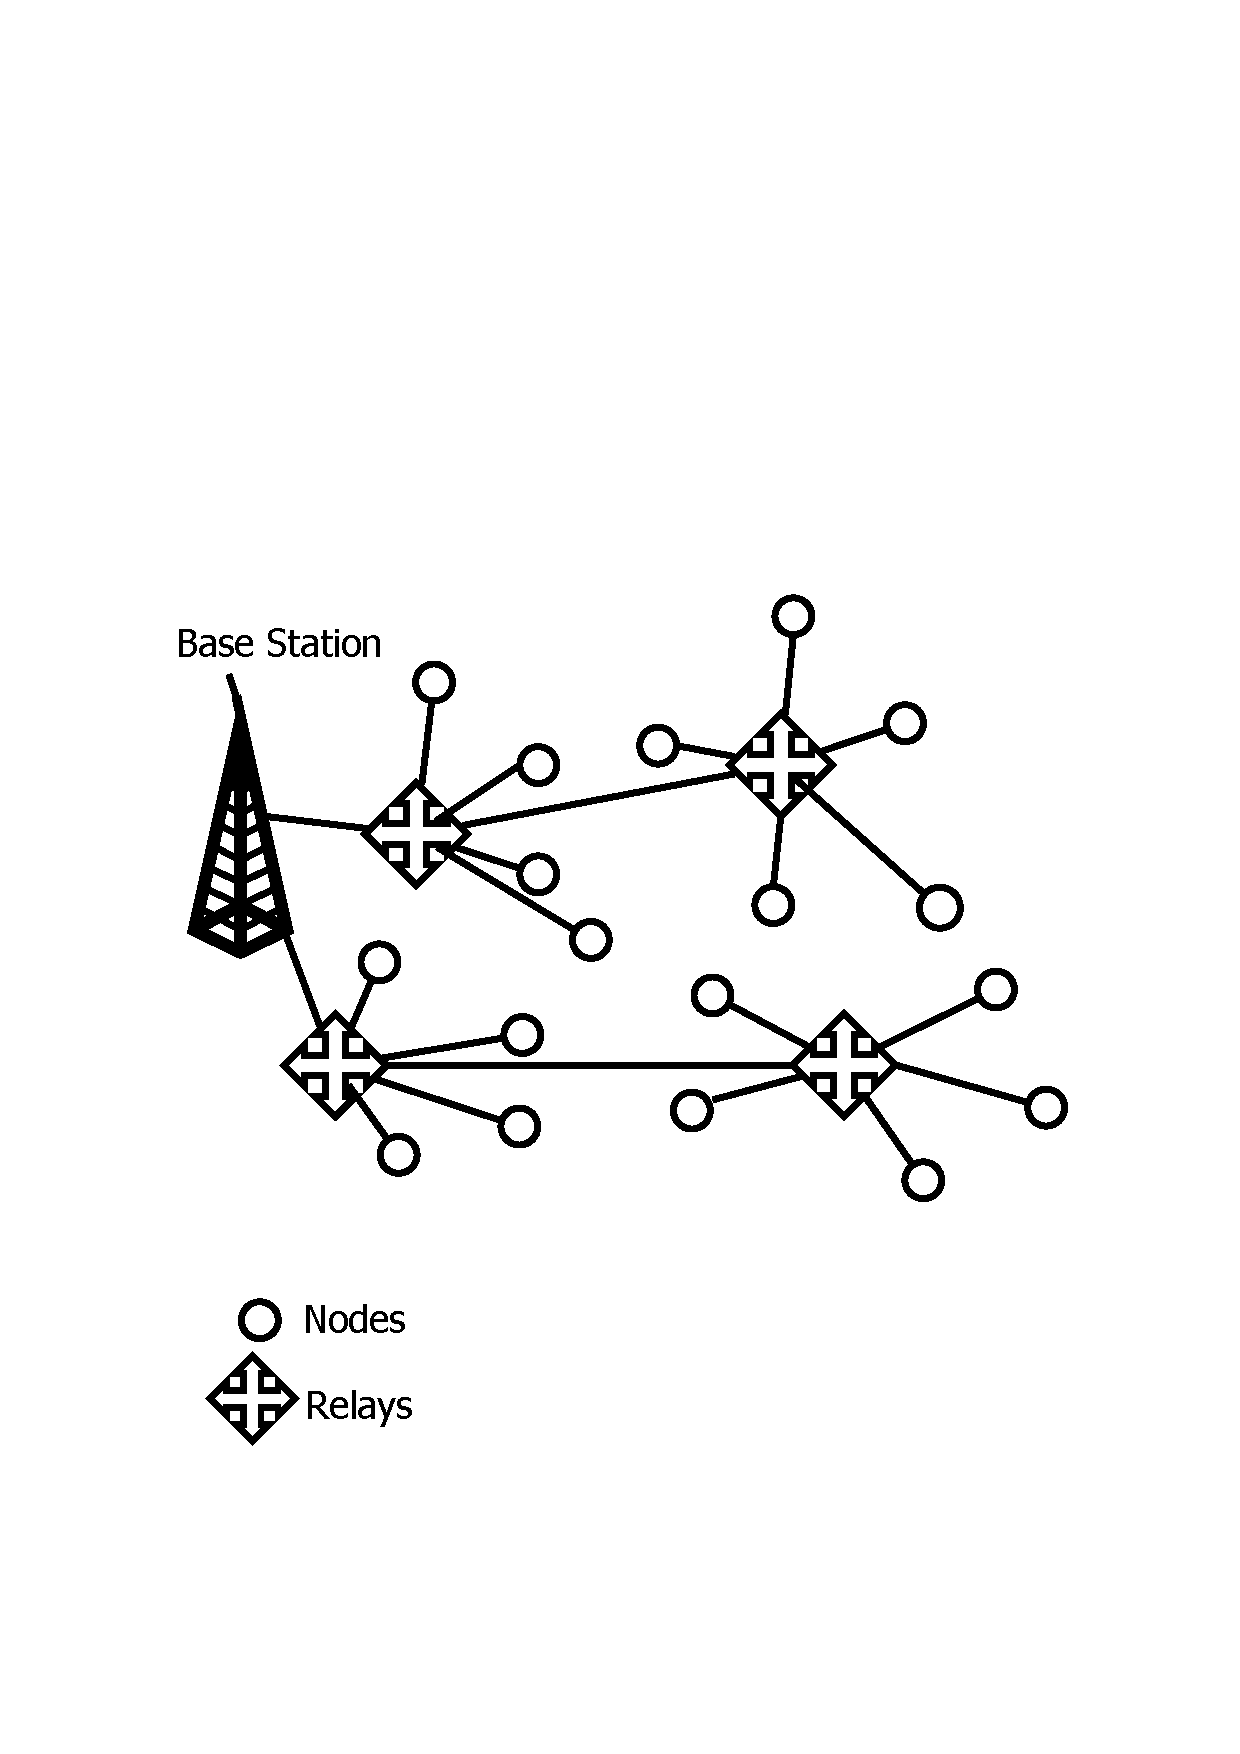
\includegraphics[trim= 0 150  0 150, clip, width=0.4\textwidth]{Figure1.pdf}</span></td>
      </tr>
      <tr>
        <td id="L974" class="blob-num js-line-number" data-line-number="974"></td>
        <td id="LC974" class="blob-code blob-code-inner js-file-line">    <span class="pl-c1">\includegraphics</span>[trim= 150 200 150 200, clip, width=0.4<span class="pl-c1">\textwidth</span>]{figure_barplot.pdf}</td>
      </tr>
      <tr>
        <td id="L975" class="blob-num js-line-number" data-line-number="975"></td>
        <td id="LC975" class="blob-code blob-code-inner js-file-line">    <span class="pl-c1">\caption</span>{Simulation results: (a) average latency and (b) packet delivery ratio (PDR). </td>
      </tr>
      <tr>
        <td id="L976" class="blob-num js-line-number" data-line-number="976"></td>
        <td id="LC976" class="blob-code blob-code-inner js-file-line">    R and M denote the number of relay nodes and the mobility type, respectively}</td>
      </tr>
      <tr>
        <td id="L977" class="blob-num js-line-number" data-line-number="977"></td>
        <td id="LC977" class="blob-code blob-code-inner js-file-line">    <span class="pl-c1">\label</span>{fig:results_bar}</td>
      </tr>
      <tr>
        <td id="L978" class="blob-num js-line-number" data-line-number="978"></td>
        <td id="LC978" class="blob-code blob-code-inner js-file-line"><span class="pl-c1">\end</span>{figure}</td>
      </tr>
      <tr>
        <td id="L979" class="blob-num js-line-number" data-line-number="979"></td>
        <td id="LC979" class="blob-code blob-code-inner js-file-line">
</td>
      </tr>
      <tr>
        <td id="L980" class="blob-num js-line-number" data-line-number="980"></td>
        <td id="LC980" class="blob-code blob-code-inner js-file-line">From the powertrace tool, we can estimate the average current consumption of</td>
      </tr>
      <tr>
        <td id="L981" class="blob-num js-line-number" data-line-number="981"></td>
        <td id="LC981" class="blob-code blob-code-inner js-file-line">the sensor node.  In our simulations we obtained an average current consumption</td>
      </tr>
      <tr>
        <td id="L982" class="blob-num js-line-number" data-line-number="982"></td>
        <td id="LC982" class="blob-code blob-code-inner js-file-line">of <span class="pl-s"><span class="pl-pds">$</span>I_{SN} = <span class="pl-c1">0.93</span> mA<span class="pl-pds">$</span></span>.  If we presume the use of two Energizer E91 Alkaline AA</td>
      </tr>
      <tr>
        <td id="L983" class="blob-num js-line-number" data-line-number="983"></td>
        <td id="LC983" class="blob-code blob-code-inner js-file-line">batteries~<span class="pl-c1">\cite</span>{EnergizerBattery}, which has a capacity of <span class="pl-s"><span class="pl-pds">$</span>C_{battery} = <span class="pl-c1">2500</span></span></td>
      </tr>
      <tr>
        <td id="L984" class="blob-num js-line-number" data-line-number="984"></td>
        <td id="LC984" class="blob-code blob-code-inner js-file-line"><span class="pl-s">mAh<span class="pl-pds">$</span></span>, we can, then, estimate the expected lifetime of a sensor node using</td>
      </tr>
      <tr>
        <td id="L985" class="blob-num js-line-number" data-line-number="985"></td>
        <td id="LC985" class="blob-code blob-code-inner js-file-line">Eq.~<span class="pl-c1">\ref</span>{eq:lifetime}:</td>
      </tr>
      <tr>
        <td id="L986" class="blob-num js-line-number" data-line-number="986"></td>
        <td id="LC986" class="blob-code blob-code-inner js-file-line">
</td>
      </tr>
      <tr>
        <td id="L987" class="blob-num js-line-number" data-line-number="987"></td>
        <td id="LC987" class="blob-code blob-code-inner js-file-line"><span class="pl-c1">\begin</span>{equation}</td>
      </tr>
      <tr>
        <td id="L988" class="blob-num js-line-number" data-line-number="988"></td>
        <td id="LC988" class="blob-code blob-code-inner js-file-line"><span class="pl-c1">\label</span>{eq:lifetime}</td>
      </tr>
      <tr>
        <td id="L989" class="blob-num js-line-number" data-line-number="989"></td>
        <td id="LC989" class="blob-code blob-code-inner js-file-line">T = <span class="pl-c1">\frac</span>{C_{battery}}{I_{SN}}</td>
      </tr>
      <tr>
        <td id="L990" class="blob-num js-line-number" data-line-number="990"></td>
        <td id="LC990" class="blob-code blob-code-inner js-file-line"><span class="pl-c1">\end</span>{equation}</td>
      </tr>
      <tr>
        <td id="L991" class="blob-num js-line-number" data-line-number="991"></td>
        <td id="LC991" class="blob-code blob-code-inner js-file-line">
</td>
      </tr>
      <tr>
        <td id="L992" class="blob-num js-line-number" data-line-number="992"></td>
        <td id="LC992" class="blob-code blob-code-inner js-file-line">With this calculation we obtain an expected average lifetime of approx. 112 days. This value, </td>
      </tr>
      <tr>
        <td id="L993" class="blob-num js-line-number" data-line-number="993"></td>
        <td id="LC993" class="blob-code blob-code-inner js-file-line">however, should be treated carefully and no final conclusion should be drawn</td>
      </tr>
      <tr>
        <td id="L994" class="blob-num js-line-number" data-line-number="994"></td>
        <td id="LC994" class="blob-code blob-code-inner js-file-line">from it. First of all this is only a simulation based estimation, in which we</td>
      </tr>
      <tr>
        <td id="L995" class="blob-num js-line-number" data-line-number="995"></td>
        <td id="LC995" class="blob-code blob-code-inner js-file-line">increased the sampling frequency of data generation. In addition, the use of</td>
      </tr>
      <tr>
        <td id="L996" class="blob-num js-line-number" data-line-number="996"></td>
        <td id="LC996" class="blob-code blob-code-inner js-file-line">this tool requires more CPU usages which leads to higher consumption. On the</td>
      </tr>
      <tr>
        <td id="L997" class="blob-num js-line-number" data-line-number="997"></td>
        <td id="LC997" class="blob-code blob-code-inner js-file-line">other hand, though, we haven&#39;t included the current consumption of real sensors</td>
      </tr>
      <tr>
        <td id="L998" class="blob-num js-line-number" data-line-number="998"></td>
        <td id="LC998" class="blob-code blob-code-inner js-file-line">into the estimation. </td>
      </tr>
      <tr>
        <td id="L999" class="blob-num js-line-number" data-line-number="999"></td>
        <td id="LC999" class="blob-code blob-code-inner js-file-line">
</td>
      </tr>
      <tr>
        <td id="L1000" class="blob-num js-line-number" data-line-number="1000"></td>
        <td id="LC1000" class="blob-code blob-code-inner js-file-line"><span class="pl-c1">\subsection</span>{Discussion} <span class="pl-c1">\label</span>{sec:discussion}</td>
      </tr>
      <tr>
        <td id="L1001" class="blob-num js-line-number" data-line-number="1001"></td>
        <td id="LC1001" class="blob-code blob-code-inner js-file-line">
</td>
      </tr>
      <tr>
        <td id="L1002" class="blob-num js-line-number" data-line-number="1002"></td>
        <td id="LC1002" class="blob-code blob-code-inner js-file-line"><span class="pl-c1">\section</span>{Conclusion}</td>
      </tr>
      <tr>
        <td id="L1003" class="blob-num js-line-number" data-line-number="1003"></td>
        <td id="LC1003" class="blob-code blob-code-inner js-file-line">
</td>
      </tr>
      <tr>
        <td id="L1004" class="blob-num js-line-number" data-line-number="1004"></td>
        <td id="LC1004" class="blob-code blob-code-inner js-file-line"><span class="pl-c1">\section</span>{Future Work}</td>
      </tr>
      <tr>
        <td id="L1005" class="blob-num js-line-number" data-line-number="1005"></td>
        <td id="LC1005" class="blob-code blob-code-inner js-file-line">
</td>
      </tr>
      <tr>
        <td id="L1006" class="blob-num js-line-number" data-line-number="1006"></td>
        <td id="LC1006" class="blob-code blob-code-inner js-file-line"><span class="pl-c">%\section{Work Plan}</span></td>
      </tr>
      <tr>
        <td id="L1007" class="blob-num js-line-number" data-line-number="1007"></td>
        <td id="LC1007" class="blob-code blob-code-inner js-file-line">
</td>
      </tr>
      <tr>
        <td id="L1008" class="blob-num js-line-number" data-line-number="1008"></td>
        <td id="LC1008" class="blob-code blob-code-inner js-file-line"><span class="pl-c">% An example of a floating figure using the graphicx package.</span></td>
      </tr>
      <tr>
        <td id="L1009" class="blob-num js-line-number" data-line-number="1009"></td>
        <td id="LC1009" class="blob-code blob-code-inner js-file-line"><span class="pl-c">% Note that \label must occur AFTER (or within) \caption.</span></td>
      </tr>
      <tr>
        <td id="L1010" class="blob-num js-line-number" data-line-number="1010"></td>
        <td id="LC1010" class="blob-code blob-code-inner js-file-line"><span class="pl-c">% For figures, \caption should occur after the \includegraphics.</span></td>
      </tr>
      <tr>
        <td id="L1011" class="blob-num js-line-number" data-line-number="1011"></td>
        <td id="LC1011" class="blob-code blob-code-inner js-file-line"><span class="pl-c">% Note that IEEEtran v1.7 and later has special internal code that</span></td>
      </tr>
      <tr>
        <td id="L1012" class="blob-num js-line-number" data-line-number="1012"></td>
        <td id="LC1012" class="blob-code blob-code-inner js-file-line"><span class="pl-c">% is designed to preserve the operation of \label within \caption</span></td>
      </tr>
      <tr>
        <td id="L1013" class="blob-num js-line-number" data-line-number="1013"></td>
        <td id="LC1013" class="blob-code blob-code-inner js-file-line"><span class="pl-c">% even when the captionsoff option is in effect. However, because</span></td>
      </tr>
      <tr>
        <td id="L1014" class="blob-num js-line-number" data-line-number="1014"></td>
        <td id="LC1014" class="blob-code blob-code-inner js-file-line"><span class="pl-c">% of issues like this, it may be the safest practice to put all your</span></td>
      </tr>
      <tr>
        <td id="L1015" class="blob-num js-line-number" data-line-number="1015"></td>
        <td id="LC1015" class="blob-code blob-code-inner js-file-line"><span class="pl-c">% \label just after \caption rather than within \caption{}.</span></td>
      </tr>
      <tr>
        <td id="L1016" class="blob-num js-line-number" data-line-number="1016"></td>
        <td id="LC1016" class="blob-code blob-code-inner js-file-line"><span class="pl-c">%</span></td>
      </tr>
      <tr>
        <td id="L1017" class="blob-num js-line-number" data-line-number="1017"></td>
        <td id="LC1017" class="blob-code blob-code-inner js-file-line"><span class="pl-c">% Reminder: the &quot;draftcls&quot; or &quot;draftclsnofoot&quot;, not &quot;draft&quot;, class</span></td>
      </tr>
      <tr>
        <td id="L1018" class="blob-num js-line-number" data-line-number="1018"></td>
        <td id="LC1018" class="blob-code blob-code-inner js-file-line"><span class="pl-c">% option should be used if it is desired that the figures are to be</span></td>
      </tr>
      <tr>
        <td id="L1019" class="blob-num js-line-number" data-line-number="1019"></td>
        <td id="LC1019" class="blob-code blob-code-inner js-file-line"><span class="pl-c">% displayed while in draft mode.</span></td>
      </tr>
      <tr>
        <td id="L1020" class="blob-num js-line-number" data-line-number="1020"></td>
        <td id="LC1020" class="blob-code blob-code-inner js-file-line"><span class="pl-c">%</span></td>
      </tr>
      <tr>
        <td id="L1021" class="blob-num js-line-number" data-line-number="1021"></td>
        <td id="LC1021" class="blob-code blob-code-inner js-file-line"><span class="pl-c">%\begin{figure}[!t]</span></td>
      </tr>
      <tr>
        <td id="L1022" class="blob-num js-line-number" data-line-number="1022"></td>
        <td id="LC1022" class="blob-code blob-code-inner js-file-line"><span class="pl-c">%\centering</span></td>
      </tr>
      <tr>
        <td id="L1023" class="blob-num js-line-number" data-line-number="1023"></td>
        <td id="LC1023" class="blob-code blob-code-inner js-file-line"><span class="pl-c">%\includegraphics[width=2.5in]{myfigure}</span></td>
      </tr>
      <tr>
        <td id="L1024" class="blob-num js-line-number" data-line-number="1024"></td>
        <td id="LC1024" class="blob-code blob-code-inner js-file-line"><span class="pl-c">% where an .eps filename suffix will be assumed under latex, </span></td>
      </tr>
      <tr>
        <td id="L1025" class="blob-num js-line-number" data-line-number="1025"></td>
        <td id="LC1025" class="blob-code blob-code-inner js-file-line"><span class="pl-c">% and a .pdf suffix will be assumed for pdflatex; or what has been declared</span></td>
      </tr>
      <tr>
        <td id="L1026" class="blob-num js-line-number" data-line-number="1026"></td>
        <td id="LC1026" class="blob-code blob-code-inner js-file-line"><span class="pl-c">% via \DeclareGraphicsExtensions.</span></td>
      </tr>
      <tr>
        <td id="L1027" class="blob-num js-line-number" data-line-number="1027"></td>
        <td id="LC1027" class="blob-code blob-code-inner js-file-line"><span class="pl-c">%\caption{Simulation results for the network.}</span></td>
      </tr>
      <tr>
        <td id="L1028" class="blob-num js-line-number" data-line-number="1028"></td>
        <td id="LC1028" class="blob-code blob-code-inner js-file-line"><span class="pl-c">%\label{fig_sim}</span></td>
      </tr>
      <tr>
        <td id="L1029" class="blob-num js-line-number" data-line-number="1029"></td>
        <td id="LC1029" class="blob-code blob-code-inner js-file-line"><span class="pl-c">%\end{figure}</span></td>
      </tr>
      <tr>
        <td id="L1030" class="blob-num js-line-number" data-line-number="1030"></td>
        <td id="LC1030" class="blob-code blob-code-inner js-file-line">
</td>
      </tr>
      <tr>
        <td id="L1031" class="blob-num js-line-number" data-line-number="1031"></td>
        <td id="LC1031" class="blob-code blob-code-inner js-file-line"><span class="pl-c">% Note that the IEEE typically puts floats only at the top, even when this</span></td>
      </tr>
      <tr>
        <td id="L1032" class="blob-num js-line-number" data-line-number="1032"></td>
        <td id="LC1032" class="blob-code blob-code-inner js-file-line"><span class="pl-c">% results in a large percentage of a column being occupied by floats.</span></td>
      </tr>
      <tr>
        <td id="L1033" class="blob-num js-line-number" data-line-number="1033"></td>
        <td id="LC1033" class="blob-code blob-code-inner js-file-line">
</td>
      </tr>
      <tr>
        <td id="L1034" class="blob-num js-line-number" data-line-number="1034"></td>
        <td id="LC1034" class="blob-code blob-code-inner js-file-line">
</td>
      </tr>
      <tr>
        <td id="L1035" class="blob-num js-line-number" data-line-number="1035"></td>
        <td id="LC1035" class="blob-code blob-code-inner js-file-line"><span class="pl-c">% An example of a double column floating figure using two subfigures.</span></td>
      </tr>
      <tr>
        <td id="L1036" class="blob-num js-line-number" data-line-number="1036"></td>
        <td id="LC1036" class="blob-code blob-code-inner js-file-line"><span class="pl-c">% (The subfig.sty package must be loaded for this to work.)</span></td>
      </tr>
      <tr>
        <td id="L1037" class="blob-num js-line-number" data-line-number="1037"></td>
        <td id="LC1037" class="blob-code blob-code-inner js-file-line"><span class="pl-c">% The subfigure \label commands are set within each subfloat command,</span></td>
      </tr>
      <tr>
        <td id="L1038" class="blob-num js-line-number" data-line-number="1038"></td>
        <td id="LC1038" class="blob-code blob-code-inner js-file-line"><span class="pl-c">% and the \label for the overall figure must come after \caption.</span></td>
      </tr>
      <tr>
        <td id="L1039" class="blob-num js-line-number" data-line-number="1039"></td>
        <td id="LC1039" class="blob-code blob-code-inner js-file-line"><span class="pl-c">% \hfil is used as a separator to get equal spacing.</span></td>
      </tr>
      <tr>
        <td id="L1040" class="blob-num js-line-number" data-line-number="1040"></td>
        <td id="LC1040" class="blob-code blob-code-inner js-file-line"><span class="pl-c">% Watch out that the combined width of all the subfigures on a </span></td>
      </tr>
      <tr>
        <td id="L1041" class="blob-num js-line-number" data-line-number="1041"></td>
        <td id="LC1041" class="blob-code blob-code-inner js-file-line"><span class="pl-c">% line do not exceed the text width or a line break will occur.</span></td>
      </tr>
      <tr>
        <td id="L1042" class="blob-num js-line-number" data-line-number="1042"></td>
        <td id="LC1042" class="blob-code blob-code-inner js-file-line"><span class="pl-c">%</span></td>
      </tr>
      <tr>
        <td id="L1043" class="blob-num js-line-number" data-line-number="1043"></td>
        <td id="LC1043" class="blob-code blob-code-inner js-file-line"><span class="pl-c">%\begin{figure*}[!t]</span></td>
      </tr>
      <tr>
        <td id="L1044" class="blob-num js-line-number" data-line-number="1044"></td>
        <td id="LC1044" class="blob-code blob-code-inner js-file-line"><span class="pl-c">%\centering</span></td>
      </tr>
      <tr>
        <td id="L1045" class="blob-num js-line-number" data-line-number="1045"></td>
        <td id="LC1045" class="blob-code blob-code-inner js-file-line"><span class="pl-c">%\subfloat[Case I]{\includegraphics[width=2.5in]{box}%</span></td>
      </tr>
      <tr>
        <td id="L1046" class="blob-num js-line-number" data-line-number="1046"></td>
        <td id="LC1046" class="blob-code blob-code-inner js-file-line"><span class="pl-c">%\label{fig_first_case}}</span></td>
      </tr>
      <tr>
        <td id="L1047" class="blob-num js-line-number" data-line-number="1047"></td>
        <td id="LC1047" class="blob-code blob-code-inner js-file-line"><span class="pl-c">%\hfil</span></td>
      </tr>
      <tr>
        <td id="L1048" class="blob-num js-line-number" data-line-number="1048"></td>
        <td id="LC1048" class="blob-code blob-code-inner js-file-line"><span class="pl-c">%\subfloat[Case II]{\includegraphics[width=2.5in]{box}%</span></td>
      </tr>
      <tr>
        <td id="L1049" class="blob-num js-line-number" data-line-number="1049"></td>
        <td id="LC1049" class="blob-code blob-code-inner js-file-line"><span class="pl-c">%\label{fig_second_case}}</span></td>
      </tr>
      <tr>
        <td id="L1050" class="blob-num js-line-number" data-line-number="1050"></td>
        <td id="LC1050" class="blob-code blob-code-inner js-file-line"><span class="pl-c">%\caption{Simulation results for the network.}</span></td>
      </tr>
      <tr>
        <td id="L1051" class="blob-num js-line-number" data-line-number="1051"></td>
        <td id="LC1051" class="blob-code blob-code-inner js-file-line"><span class="pl-c">%\label{fig_sim}</span></td>
      </tr>
      <tr>
        <td id="L1052" class="blob-num js-line-number" data-line-number="1052"></td>
        <td id="LC1052" class="blob-code blob-code-inner js-file-line"><span class="pl-c">%\end{figure*}</span></td>
      </tr>
      <tr>
        <td id="L1053" class="blob-num js-line-number" data-line-number="1053"></td>
        <td id="LC1053" class="blob-code blob-code-inner js-file-line"><span class="pl-c">%</span></td>
      </tr>
      <tr>
        <td id="L1054" class="blob-num js-line-number" data-line-number="1054"></td>
        <td id="LC1054" class="blob-code blob-code-inner js-file-line"><span class="pl-c">% Note that often IEEE papers with subfigures do not employ subfigure</span></td>
      </tr>
      <tr>
        <td id="L1055" class="blob-num js-line-number" data-line-number="1055"></td>
        <td id="LC1055" class="blob-code blob-code-inner js-file-line"><span class="pl-c">% captions (using the optional argument to \subfloat[]), but instead will</span></td>
      </tr>
      <tr>
        <td id="L1056" class="blob-num js-line-number" data-line-number="1056"></td>
        <td id="LC1056" class="blob-code blob-code-inner js-file-line"><span class="pl-c">% reference/describe all of them (a), (b), etc., within the main caption.</span></td>
      </tr>
      <tr>
        <td id="L1057" class="blob-num js-line-number" data-line-number="1057"></td>
        <td id="LC1057" class="blob-code blob-code-inner js-file-line"><span class="pl-c">% Be aware that for subfig.sty to generate the (a), (b), etc., subfigure</span></td>
      </tr>
      <tr>
        <td id="L1058" class="blob-num js-line-number" data-line-number="1058"></td>
        <td id="LC1058" class="blob-code blob-code-inner js-file-line"><span class="pl-c">% labels, the optional argument to \subfloat must be present. If a</span></td>
      </tr>
      <tr>
        <td id="L1059" class="blob-num js-line-number" data-line-number="1059"></td>
        <td id="LC1059" class="blob-code blob-code-inner js-file-line"><span class="pl-c">% subcaption is not desired, just leave its contents blank,</span></td>
      </tr>
      <tr>
        <td id="L1060" class="blob-num js-line-number" data-line-number="1060"></td>
        <td id="LC1060" class="blob-code blob-code-inner js-file-line"><span class="pl-c">% e.g., \subfloat[].</span></td>
      </tr>
      <tr>
        <td id="L1061" class="blob-num js-line-number" data-line-number="1061"></td>
        <td id="LC1061" class="blob-code blob-code-inner js-file-line">
</td>
      </tr>
      <tr>
        <td id="L1062" class="blob-num js-line-number" data-line-number="1062"></td>
        <td id="LC1062" class="blob-code blob-code-inner js-file-line">
</td>
      </tr>
      <tr>
        <td id="L1063" class="blob-num js-line-number" data-line-number="1063"></td>
        <td id="LC1063" class="blob-code blob-code-inner js-file-line"><span class="pl-c">% An example of a floating table. Note that, for IEEE style tables, the</span></td>
      </tr>
      <tr>
        <td id="L1064" class="blob-num js-line-number" data-line-number="1064"></td>
        <td id="LC1064" class="blob-code blob-code-inner js-file-line"><span class="pl-c">% \caption command should come BEFORE the table and, given that table</span></td>
      </tr>
      <tr>
        <td id="L1065" class="blob-num js-line-number" data-line-number="1065"></td>
        <td id="LC1065" class="blob-code blob-code-inner js-file-line"><span class="pl-c">% captions serve much like titles, are usually capitalized except for words</span></td>
      </tr>
      <tr>
        <td id="L1066" class="blob-num js-line-number" data-line-number="1066"></td>
        <td id="LC1066" class="blob-code blob-code-inner js-file-line"><span class="pl-c">% such as a, an, and, as, at, but, by, for, in, nor, of, on, or, the, to</span></td>
      </tr>
      <tr>
        <td id="L1067" class="blob-num js-line-number" data-line-number="1067"></td>
        <td id="LC1067" class="blob-code blob-code-inner js-file-line"><span class="pl-c">% and up, which are usually not capitalized unless they are the first or</span></td>
      </tr>
      <tr>
        <td id="L1068" class="blob-num js-line-number" data-line-number="1068"></td>
        <td id="LC1068" class="blob-code blob-code-inner js-file-line"><span class="pl-c">% last word of the caption. Table text will default to \footnotesize as</span></td>
      </tr>
      <tr>
        <td id="L1069" class="blob-num js-line-number" data-line-number="1069"></td>
        <td id="LC1069" class="blob-code blob-code-inner js-file-line"><span class="pl-c">% the IEEE normally uses this smaller font for tables.</span></td>
      </tr>
      <tr>
        <td id="L1070" class="blob-num js-line-number" data-line-number="1070"></td>
        <td id="LC1070" class="blob-code blob-code-inner js-file-line"><span class="pl-c">% The \label must come after \caption as always.</span></td>
      </tr>
      <tr>
        <td id="L1071" class="blob-num js-line-number" data-line-number="1071"></td>
        <td id="LC1071" class="blob-code blob-code-inner js-file-line"><span class="pl-c">%</span></td>
      </tr>
      <tr>
        <td id="L1072" class="blob-num js-line-number" data-line-number="1072"></td>
        <td id="LC1072" class="blob-code blob-code-inner js-file-line"><span class="pl-c">%\begin{table}[!t]</span></td>
      </tr>
      <tr>
        <td id="L1073" class="blob-num js-line-number" data-line-number="1073"></td>
        <td id="LC1073" class="blob-code blob-code-inner js-file-line"><span class="pl-c">%% increase table row spacing, adjust to taste</span></td>
      </tr>
      <tr>
        <td id="L1074" class="blob-num js-line-number" data-line-number="1074"></td>
        <td id="LC1074" class="blob-code blob-code-inner js-file-line"><span class="pl-c">%\renewcommand{\arraystretch}{1.3}</span></td>
      </tr>
      <tr>
        <td id="L1075" class="blob-num js-line-number" data-line-number="1075"></td>
        <td id="LC1075" class="blob-code blob-code-inner js-file-line"><span class="pl-c">% if using array.sty, it might be a good idea to tweak the value of</span></td>
      </tr>
      <tr>
        <td id="L1076" class="blob-num js-line-number" data-line-number="1076"></td>
        <td id="LC1076" class="blob-code blob-code-inner js-file-line"><span class="pl-c">% \extrarowheight as needed to properly center the text within the cells</span></td>
      </tr>
      <tr>
        <td id="L1077" class="blob-num js-line-number" data-line-number="1077"></td>
        <td id="LC1077" class="blob-code blob-code-inner js-file-line"><span class="pl-c">%\caption{An Example of a Table}</span></td>
      </tr>
      <tr>
        <td id="L1078" class="blob-num js-line-number" data-line-number="1078"></td>
        <td id="LC1078" class="blob-code blob-code-inner js-file-line"><span class="pl-c">%\label{table_example}</span></td>
      </tr>
      <tr>
        <td id="L1079" class="blob-num js-line-number" data-line-number="1079"></td>
        <td id="LC1079" class="blob-code blob-code-inner js-file-line"><span class="pl-c">%\centering</span></td>
      </tr>
      <tr>
        <td id="L1080" class="blob-num js-line-number" data-line-number="1080"></td>
        <td id="LC1080" class="blob-code blob-code-inner js-file-line"><span class="pl-c">%% Some packages, such as MDW tools, offer better commands for making tables</span></td>
      </tr>
      <tr>
        <td id="L1081" class="blob-num js-line-number" data-line-number="1081"></td>
        <td id="LC1081" class="blob-code blob-code-inner js-file-line"><span class="pl-c">%% than the plain LaTeX2e tabular which is used here.</span></td>
      </tr>
      <tr>
        <td id="L1082" class="blob-num js-line-number" data-line-number="1082"></td>
        <td id="LC1082" class="blob-code blob-code-inner js-file-line"><span class="pl-c">%\begin{tabular}{|c||c|}</span></td>
      </tr>
      <tr>
        <td id="L1083" class="blob-num js-line-number" data-line-number="1083"></td>
        <td id="LC1083" class="blob-code blob-code-inner js-file-line"><span class="pl-c">%\hline</span></td>
      </tr>
      <tr>
        <td id="L1084" class="blob-num js-line-number" data-line-number="1084"></td>
        <td id="LC1084" class="blob-code blob-code-inner js-file-line"><span class="pl-c">%One &amp; Two\\</span></td>
      </tr>
      <tr>
        <td id="L1085" class="blob-num js-line-number" data-line-number="1085"></td>
        <td id="LC1085" class="blob-code blob-code-inner js-file-line"><span class="pl-c">%\hline</span></td>
      </tr>
      <tr>
        <td id="L1086" class="blob-num js-line-number" data-line-number="1086"></td>
        <td id="LC1086" class="blob-code blob-code-inner js-file-line"><span class="pl-c">%Three &amp; Four\\</span></td>
      </tr>
      <tr>
        <td id="L1087" class="blob-num js-line-number" data-line-number="1087"></td>
        <td id="LC1087" class="blob-code blob-code-inner js-file-line"><span class="pl-c">%\hline</span></td>
      </tr>
      <tr>
        <td id="L1088" class="blob-num js-line-number" data-line-number="1088"></td>
        <td id="LC1088" class="blob-code blob-code-inner js-file-line"><span class="pl-c">%\end{tabular}</span></td>
      </tr>
      <tr>
        <td id="L1089" class="blob-num js-line-number" data-line-number="1089"></td>
        <td id="LC1089" class="blob-code blob-code-inner js-file-line"><span class="pl-c">%\end{table}</span></td>
      </tr>
      <tr>
        <td id="L1090" class="blob-num js-line-number" data-line-number="1090"></td>
        <td id="LC1090" class="blob-code blob-code-inner js-file-line">
</td>
      </tr>
      <tr>
        <td id="L1091" class="blob-num js-line-number" data-line-number="1091"></td>
        <td id="LC1091" class="blob-code blob-code-inner js-file-line">
</td>
      </tr>
      <tr>
        <td id="L1092" class="blob-num js-line-number" data-line-number="1092"></td>
        <td id="LC1092" class="blob-code blob-code-inner js-file-line"><span class="pl-c">% Note that the IEEE does not put floats in the very first column</span></td>
      </tr>
      <tr>
        <td id="L1093" class="blob-num js-line-number" data-line-number="1093"></td>
        <td id="LC1093" class="blob-code blob-code-inner js-file-line"><span class="pl-c">% - or typically anywhere on the first page for that matter. Also,</span></td>
      </tr>
      <tr>
        <td id="L1094" class="blob-num js-line-number" data-line-number="1094"></td>
        <td id="LC1094" class="blob-code blob-code-inner js-file-line"><span class="pl-c">% in-text middle (&quot;here&quot;) positioning is typically not used, but it</span></td>
      </tr>
      <tr>
        <td id="L1095" class="blob-num js-line-number" data-line-number="1095"></td>
        <td id="LC1095" class="blob-code blob-code-inner js-file-line"><span class="pl-c">% is allowed and encouraged for Computer Society conferences (but</span></td>
      </tr>
      <tr>
        <td id="L1096" class="blob-num js-line-number" data-line-number="1096"></td>
        <td id="LC1096" class="blob-code blob-code-inner js-file-line"><span class="pl-c">% not Computer Society journals). Most IEEE journals/conferences use</span></td>
      </tr>
      <tr>
        <td id="L1097" class="blob-num js-line-number" data-line-number="1097"></td>
        <td id="LC1097" class="blob-code blob-code-inner js-file-line"><span class="pl-c">% top floats exclusively. </span></td>
      </tr>
      <tr>
        <td id="L1098" class="blob-num js-line-number" data-line-number="1098"></td>
        <td id="LC1098" class="blob-code blob-code-inner js-file-line"><span class="pl-c">% Note that, LaTeX2e, unlike IEEE journals/conferences, places</span></td>
      </tr>
      <tr>
        <td id="L1099" class="blob-num js-line-number" data-line-number="1099"></td>
        <td id="LC1099" class="blob-code blob-code-inner js-file-line"><span class="pl-c">% footnotes above bottom floats. This can be corrected via the</span></td>
      </tr>
      <tr>
        <td id="L1100" class="blob-num js-line-number" data-line-number="1100"></td>
        <td id="LC1100" class="blob-code blob-code-inner js-file-line"><span class="pl-c">% \fnbelowfloat command of the stfloats package.</span></td>
      </tr>
      <tr>
        <td id="L1101" class="blob-num js-line-number" data-line-number="1101"></td>
        <td id="LC1101" class="blob-code blob-code-inner js-file-line">
</td>
      </tr>
      <tr>
        <td id="L1102" class="blob-num js-line-number" data-line-number="1102"></td>
        <td id="LC1102" class="blob-code blob-code-inner js-file-line">
</td>
      </tr>
      <tr>
        <td id="L1103" class="blob-num js-line-number" data-line-number="1103"></td>
        <td id="LC1103" class="blob-code blob-code-inner js-file-line"><span class="pl-c">% conference papers do not normally have an appendix</span></td>
      </tr>
      <tr>
        <td id="L1104" class="blob-num js-line-number" data-line-number="1104"></td>
        <td id="LC1104" class="blob-code blob-code-inner js-file-line">
</td>
      </tr>
      <tr>
        <td id="L1105" class="blob-num js-line-number" data-line-number="1105"></td>
        <td id="LC1105" class="blob-code blob-code-inner js-file-line"><span class="pl-c">% trigger a \newpage just before the given reference</span></td>
      </tr>
      <tr>
        <td id="L1106" class="blob-num js-line-number" data-line-number="1106"></td>
        <td id="LC1106" class="blob-code blob-code-inner js-file-line"><span class="pl-c">% number - used to balance the columns on the last page</span></td>
      </tr>
      <tr>
        <td id="L1107" class="blob-num js-line-number" data-line-number="1107"></td>
        <td id="LC1107" class="blob-code blob-code-inner js-file-line"><span class="pl-c">% adjust value as needed - may need to be readjusted if</span></td>
      </tr>
      <tr>
        <td id="L1108" class="blob-num js-line-number" data-line-number="1108"></td>
        <td id="LC1108" class="blob-code blob-code-inner js-file-line"><span class="pl-c">% the document is modified later</span></td>
      </tr>
      <tr>
        <td id="L1109" class="blob-num js-line-number" data-line-number="1109"></td>
        <td id="LC1109" class="blob-code blob-code-inner js-file-line"><span class="pl-c">%\IEEEtriggeratref{8}</span></td>
      </tr>
      <tr>
        <td id="L1110" class="blob-num js-line-number" data-line-number="1110"></td>
        <td id="LC1110" class="blob-code blob-code-inner js-file-line"><span class="pl-c">% The &quot;triggered&quot; command can be changed if desired:</span></td>
      </tr>
      <tr>
        <td id="L1111" class="blob-num js-line-number" data-line-number="1111"></td>
        <td id="LC1111" class="blob-code blob-code-inner js-file-line"><span class="pl-c">%\IEEEtriggercmd{\enlargethispage{-5in}}</span></td>
      </tr>
      <tr>
        <td id="L1112" class="blob-num js-line-number" data-line-number="1112"></td>
        <td id="LC1112" class="blob-code blob-code-inner js-file-line">
</td>
      </tr>
      <tr>
        <td id="L1113" class="blob-num js-line-number" data-line-number="1113"></td>
        <td id="LC1113" class="blob-code blob-code-inner js-file-line"><span class="pl-c">% references section</span></td>
      </tr>
      <tr>
        <td id="L1114" class="blob-num js-line-number" data-line-number="1114"></td>
        <td id="LC1114" class="blob-code blob-code-inner js-file-line">
</td>
      </tr>
      <tr>
        <td id="L1115" class="blob-num js-line-number" data-line-number="1115"></td>
        <td id="LC1115" class="blob-code blob-code-inner js-file-line"><span class="pl-c">% can use a bibliography generated by BibTeX as a .bbl file</span></td>
      </tr>
      <tr>
        <td id="L1116" class="blob-num js-line-number" data-line-number="1116"></td>
        <td id="LC1116" class="blob-code blob-code-inner js-file-line"><span class="pl-c">% BibTeX documentation can be easily obtained at:</span></td>
      </tr>
      <tr>
        <td id="L1117" class="blob-num js-line-number" data-line-number="1117"></td>
        <td id="LC1117" class="blob-code blob-code-inner js-file-line"><span class="pl-c">% http://mirror.ctan.org/biblio/bibtex/contrib/doc/</span></td>
      </tr>
      <tr>
        <td id="L1118" class="blob-num js-line-number" data-line-number="1118"></td>
        <td id="LC1118" class="blob-code blob-code-inner js-file-line"><span class="pl-c">% The IEEEtran BibTeX style support page is at:</span></td>
      </tr>
      <tr>
        <td id="L1119" class="blob-num js-line-number" data-line-number="1119"></td>
        <td id="LC1119" class="blob-code blob-code-inner js-file-line"><span class="pl-c">% http://www.michaelshell.org/tex/ieeetran/bibtex/</span></td>
      </tr>
      <tr>
        <td id="L1120" class="blob-num js-line-number" data-line-number="1120"></td>
        <td id="LC1120" class="blob-code blob-code-inner js-file-line"><span class="pl-c">%\bibliographystyle{IEEEtran}</span></td>
      </tr>
      <tr>
        <td id="L1121" class="blob-num js-line-number" data-line-number="1121"></td>
        <td id="LC1121" class="blob-code blob-code-inner js-file-line"><span class="pl-c">% argument is your BibTeX string definitions and bibliography database(s)</span></td>
      </tr>
      <tr>
        <td id="L1122" class="blob-num js-line-number" data-line-number="1122"></td>
        <td id="LC1122" class="blob-code blob-code-inner js-file-line"><span class="pl-c">%\bibliography{IEEEabrv,../bib/paper}</span></td>
      </tr>
      <tr>
        <td id="L1123" class="blob-num js-line-number" data-line-number="1123"></td>
        <td id="LC1123" class="blob-code blob-code-inner js-file-line"><span class="pl-c">%</span></td>
      </tr>
      <tr>
        <td id="L1124" class="blob-num js-line-number" data-line-number="1124"></td>
        <td id="LC1124" class="blob-code blob-code-inner js-file-line"><span class="pl-c">% &lt;OR&gt; manually copy in the resultant .bbl file</span></td>
      </tr>
      <tr>
        <td id="L1125" class="blob-num js-line-number" data-line-number="1125"></td>
        <td id="LC1125" class="blob-code blob-code-inner js-file-line"><span class="pl-c">% set second argument of \begin to the number of references</span></td>
      </tr>
      <tr>
        <td id="L1126" class="blob-num js-line-number" data-line-number="1126"></td>
        <td id="LC1126" class="blob-code blob-code-inner js-file-line"><span class="pl-c">% (used to reserve space for the reference number labels box)</span></td>
      </tr>
      <tr>
        <td id="L1127" class="blob-num js-line-number" data-line-number="1127"></td>
        <td id="LC1127" class="blob-code blob-code-inner js-file-line"><span class="pl-c1">\begin</span>{thebibliography}{1}</td>
      </tr>
      <tr>
        <td id="L1128" class="blob-num js-line-number" data-line-number="1128"></td>
        <td id="LC1128" class="blob-code blob-code-inner js-file-line">
</td>
      </tr>
      <tr>
        <td id="L1129" class="blob-num js-line-number" data-line-number="1129"></td>
        <td id="LC1129" class="blob-code blob-code-inner js-file-line"><span class="pl-c1">\bibitem</span>{nedgov}</td>
      </tr>
      <tr>
        <td id="L1130" class="blob-num js-line-number" data-line-number="1130"></td>
        <td id="LC1130" class="blob-code blob-code-inner js-file-line">    https://www.government.nl/topics/agriculture-and-livestock/contents/livestock-farming,</td>
      </tr>
      <tr>
        <td id="L1131" class="blob-num js-line-number" data-line-number="1131"></td>
        <td id="LC1131" class="blob-code blob-code-inner js-file-line">    taken 12:30 22 sep 2015.</td>
      </tr>
      <tr>
        <td id="L1132" class="blob-num js-line-number" data-line-number="1132"></td>
        <td id="LC1132" class="blob-code blob-code-inner js-file-line">
</td>
      </tr>
      <tr>
        <td id="L1133" class="blob-num js-line-number" data-line-number="1133"></td>
        <td id="LC1133" class="blob-code blob-code-inner js-file-line"><span class="pl-c1">\bibitem</span>{agriculturalsystems}</td>
      </tr>
      <tr>
        <td id="L1134" class="blob-num js-line-number" data-line-number="1134"></td>
        <td id="LC1134" class="blob-code blob-code-inner js-file-line">    D. B. Grigg, <span class="pl-c1">\emph</span>{The Agricultural Systems of</td>
      </tr>
      <tr>
        <td id="L1135" class="blob-num js-line-number" data-line-number="1135"></td>
        <td id="LC1135" class="blob-code blob-code-inner js-file-line">    the World: An Evolutionary Approach}, Cambridge University Press, november</td>
      </tr>
      <tr>
        <td id="L1136" class="blob-num js-line-number" data-line-number="1136"></td>
        <td id="LC1136" class="blob-code blob-code-inner js-file-line">    1974, p. 188.</td>
      </tr>
      <tr>
        <td id="L1137" class="blob-num js-line-number" data-line-number="1137"></td>
        <td id="LC1137" class="blob-code blob-code-inner js-file-line">
</td>
      </tr>
      <tr>
        <td id="L1138" class="blob-num js-line-number" data-line-number="1138"></td>
        <td id="LC1138" class="blob-code blob-code-inner js-file-line"><span class="pl-c1">\bibitem</span>{hese2014}</td>
      </tr>
      <tr>
        <td id="L1139" class="blob-num js-line-number" data-line-number="1139"></td>
        <td id="LC1139" class="blob-code blob-code-inner js-file-line">A. ~Helwatkar, D. ~Riordan and J. ~Walsh,</td>
      </tr>
      <tr>
        <td id="L1140" class="blob-num js-line-number" data-line-number="1140"></td>
        <td id="LC1140" class="blob-code blob-code-inner js-file-line"><span class="pl-c1">\emph</span>{Sensor Technology For Animal Health Monitoring},</td>
      </tr>
      <tr>
        <td id="L1141" class="blob-num js-line-number" data-line-number="1141"></td>
        <td id="LC1141" class="blob-code blob-code-inner js-file-line">Proceedings of the 8th International Conference on Sensing Technology,</td>
      </tr>
      <tr>
        <td id="L1142" class="blob-num js-line-number" data-line-number="1142"></td>
        <td id="LC1142" class="blob-code blob-code-inner js-file-line">sep, 2014.</td>
      </tr>
      <tr>
        <td id="L1143" class="blob-num js-line-number" data-line-number="1143"></td>
        <td id="LC1143" class="blob-code blob-code-inner js-file-line">
</td>
      </tr>
      <tr>
        <td id="L1144" class="blob-num js-line-number" data-line-number="1144"></td>
        <td id="LC1144" class="blob-code blob-code-inner js-file-line"><span class="pl-c1">\bibitem</span>{GU06AN}</td>
      </tr>
      <tr>
        <td id="L1145" class="blob-num js-line-number" data-line-number="1145"></td>
        <td id="LC1145" class="blob-code blob-code-inner js-file-line">Y. Guo, P. Corke, G. Poulton, T. Wark, G. Bishop-Hurley, and D. Swain, <span class="pl-c1">\emph</span>{Animal Behaviour Understanding using Wireless Sensor Networks,} in Proceedings 2006 31st IEEE Conference on Local Computer Networks, 2006, pp. 607–614.</td>
      </tr>
      <tr>
        <td id="L1146" class="blob-num js-line-number" data-line-number="1146"></td>
        <td id="LC1146" class="blob-code blob-code-inner js-file-line">
</td>
      </tr>
      <tr>
        <td id="L1147" class="blob-num js-line-number" data-line-number="1147"></td>
        <td id="LC1147" class="blob-code blob-code-inner js-file-line"><span class="pl-c1">\bibitem</span>{SM06AN}</td>
      </tr>
      <tr>
        <td id="L1148" class="blob-num js-line-number" data-line-number="1148"></td>
        <td id="LC1148" class="blob-code blob-code-inner js-file-line">K. Smith, A. Martinez, R. Craddolph, H. Erickson, D. Andresen, and S. Warren, <span class="pl-c1">\emph</span>{An Integrated Cattle Health Monitoring System,} in 28th Annual International Conference of the IEEE Engineering in Medicine and Biology Society, 2006. EMBS ’06, 2006, pp. 4659–4662.</td>
      </tr>
      <tr>
        <td id="L1149" class="blob-num js-line-number" data-line-number="1149"></td>
        <td id="LC1149" class="blob-code blob-code-inner js-file-line">
</td>
      </tr>
      <tr>
        <td id="L1150" class="blob-num js-line-number" data-line-number="1150"></td>
        <td id="LC1150" class="blob-code blob-code-inner js-file-line"><span class="pl-c1">\bibitem</span>{SO05AW}</td>
      </tr>
      <tr>
        <td id="L1151" class="blob-num js-line-number" data-line-number="1151"></td>
        <td id="LC1151" class="blob-code blob-code-inner js-file-line">A. C. de Sousa Silva, A. I. C. Arce, S. Souto, and E. J. X. Costa, <span class="pl-c1">\emph</span>{A wireless floating base sensor network for physiological responses of livestock,} Computers and Electronics in Agriculture, vol. 49, no. 2, pp. 246–254, Nov. 2005.</td>
      </tr>
      <tr>
        <td id="L1152" class="blob-num js-line-number" data-line-number="1152"></td>
        <td id="LC1152" class="blob-code blob-code-inner js-file-line">
</td>
      </tr>
      <tr>
        <td id="L1153" class="blob-num js-line-number" data-line-number="1153"></td>
        <td id="LC1153" class="blob-code blob-code-inner js-file-line"><span class="pl-c1">\bibitem</span>{KU15AZ}</td>
      </tr>
      <tr>
        <td id="L1154" class="blob-num js-line-number" data-line-number="1154"></td>
        <td id="LC1154" class="blob-code blob-code-inner js-file-line">A. Kumar and G. P. Hancke, <span class="pl-c1">\emph</span>{A Zigbee-Based Animal Health Monitoring System,} IEEE Sensors Journal, vol. 15, no. 1, pp. 610–617, Jan. 2015.</td>
      </tr>
      <tr>
        <td id="L1155" class="blob-num js-line-number" data-line-number="1155"></td>
        <td id="LC1155" class="blob-code blob-code-inner js-file-line">
</td>
      </tr>
      <tr>
        <td id="L1156" class="blob-num js-line-number" data-line-number="1156"></td>
        <td id="LC1156" class="blob-code blob-code-inner js-file-line"><span class="pl-c1">\bibitem</span>{MA14CA}</td>
      </tr>
      <tr>
        <td id="L1157" class="blob-num js-line-number" data-line-number="1157"></td>
        <td id="LC1157" class="blob-code blob-code-inner js-file-line">P. K. Mashoko Nkwari, S. Rimer, and B. S. Paul, <span class="pl-c1">\emph</span>{Cattle monitoring system using wireless sensor network in order to prevent cattle rustling,} in IST-Africa Conference Proceedings, 2014, 2014, pp. 1–10.</td>
      </tr>
      <tr>
        <td id="L1158" class="blob-num js-line-number" data-line-number="1158"></td>
        <td id="LC1158" class="blob-code blob-code-inner js-file-line">
</td>
      </tr>
      <tr>
        <td id="L1159" class="blob-num js-line-number" data-line-number="1159"></td>
        <td id="LC1159" class="blob-code blob-code-inner js-file-line"><span class="pl-c1">\bibitem</span>{HW11DE}</td>
      </tr>
      <tr>
        <td id="L1160" class="blob-num js-line-number" data-line-number="1160"></td>
        <td id="LC1160" class="blob-code blob-code-inner js-file-line">J. Hwang and H. Yoe, <span class="pl-c1">\emph</span>{Design and implementation of wireless sensor network based livestock activity monitoring system,} in Future Generation Information Technology, Springer, 2011, pp. 161–168.</td>
      </tr>
      <tr>
        <td id="L1161" class="blob-num js-line-number" data-line-number="1161"></td>
        <td id="LC1161" class="blob-code blob-code-inner js-file-line">
</td>
      </tr>
      <tr>
        <td id="L1162" class="blob-num js-line-number" data-line-number="1162"></td>
        <td id="LC1162" class="blob-code blob-code-inner js-file-line"><span class="pl-c1">\bibitem</span>{WA15IN}</td>
      </tr>
      <tr>
        <td id="L1163" class="blob-num js-line-number" data-line-number="1163"></td>
        <td id="LC1163" class="blob-code blob-code-inner js-file-line">H. Wang, B. Davies, and A. O. Fapojuwo, <span class="pl-c1">\emph</span>{Inter-wireless body area network scheduling algorithm for livestock health monitoring,} in 2015 IEEE Wireless Communications and Networking Conference (WCNC), 2015, pp. 2132–2137.</td>
      </tr>
      <tr>
        <td id="L1164" class="blob-num js-line-number" data-line-number="1164"></td>
        <td id="LC1164" class="blob-code blob-code-inner js-file-line">
</td>
      </tr>
      <tr>
        <td id="L1165" class="blob-num js-line-number" data-line-number="1165"></td>
        <td id="LC1165" class="blob-code blob-code-inner js-file-line"><span class="pl-c1">\bibitem</span>{KW12PR}</td>
      </tr>
      <tr>
        <td id="L1166" class="blob-num js-line-number" data-line-number="1166"></td>
        <td id="LC1166" class="blob-code blob-code-inner js-file-line">K. H. Kwong, T.-T. Wu, H. G. Goh, K. Sasloglou, B. Stephen, I. Glover, C. Shen, W. Du, C. Michie, and I. Andonovic, <span class="pl-c1">\emph</span>{Practical considerations for wireless sensor networks in cattle monitoring applications,} Computers and Electronics in Agriculture, vol. 81, pp. 33–44, Feb. 2012.</td>
      </tr>
      <tr>
        <td id="L1167" class="blob-num js-line-number" data-line-number="1167"></td>
        <td id="LC1167" class="blob-code blob-code-inner js-file-line">
</td>
      </tr>
      <tr>
        <td id="L1168" class="blob-num js-line-number" data-line-number="1168"></td>
        <td id="LC1168" class="blob-code blob-code-inner js-file-line"><span class="pl-c1">\bibitem</span>{PA15SO}</td>
      </tr>
      <tr>
        <td id="L1169" class="blob-num js-line-number" data-line-number="1169"></td>
        <td id="LC1169" class="blob-code blob-code-inner js-file-line">B. Panckhurst, P. Brown, K. Payne, and T. C. A. Molteno, <span class="pl-c1">\emph</span>{Solar-powered sensor for continuous monitoring of livestock position,} in 2015 IEEE Sensors Applications Symposium (SAS), 2015, pp. 1–6.</td>
      </tr>
      <tr>
        <td id="L1170" class="blob-num js-line-number" data-line-number="1170"></td>
        <td id="LC1170" class="blob-code blob-code-inner js-file-line">
</td>
      </tr>
      <tr>
        <td id="L1171" class="blob-num js-line-number" data-line-number="1171"></td>
        <td id="LC1171" class="blob-code blob-code-inner js-file-line"><span class="pl-c1">\bibitem</span>{NO13WI}</td>
      </tr>
      <tr>
        <td id="L1172" class="blob-num js-line-number" data-line-number="1172"></td>
        <td id="LC1172" class="blob-code blob-code-inner js-file-line">A. H. H. Nograles and F. S. Caluyo, <span class="pl-c1">\emph</span>{Wireless system for pregnancy detection in cows by monitoring temperature changes in body,} in 2013 IEEE 9th International Colloquium on Signal Processing and its Applications (CSPA), 2013, pp. 11–16.</td>
      </tr>
      <tr>
        <td id="L1173" class="blob-num js-line-number" data-line-number="1173"></td>
        <td id="LC1173" class="blob-code blob-code-inner js-file-line">
</td>
      </tr>
      <tr>
        <td id="L1174" class="blob-num js-line-number" data-line-number="1174"></td>
        <td id="LC1174" class="blob-code blob-code-inner js-file-line"><span class="pl-c1">\bibitem</span>{HU10ZI}</td>
      </tr>
      <tr>
        <td id="L1175" class="blob-num js-line-number" data-line-number="1175"></td>
        <td id="LC1175" class="blob-code blob-code-inner js-file-line">J. I. Huircán, C. Muñoz, H. Young, L. Von Dossow, J. Bustos, G. Vivallo, and M. Toneatti, <span class="pl-c1">\emph</span>{ZigBee-based wireless sensor network localization for cattle monitoring in grazing fields,} Computers and Electronics in Agriculture, vol. 74, no. 2, pp. 258–264, Nov. 2010.</td>
      </tr>
      <tr>
        <td id="L1176" class="blob-num js-line-number" data-line-number="1176"></td>
        <td id="LC1176" class="blob-code blob-code-inner js-file-line">
</td>
      </tr>
      <tr>
        <td id="L1177" class="blob-num js-line-number" data-line-number="1177"></td>
        <td id="LC1177" class="blob-code blob-code-inner js-file-line"><span class="pl-c1">\bibitem</span>{KW09WI}</td>
      </tr>
      <tr>
        <td id="L1178" class="blob-num js-line-number" data-line-number="1178"></td>
        <td id="LC1178" class="blob-code blob-code-inner js-file-line">K. H. Kwong, T. T. Wu, H. G. Goh, B. Stephen, M. Gilroy, C. Michie, and I. Andonovic, <span class="pl-c1">\emph</span>{Wireless sensor networks in agriculture: cattle monitoring for farming industries,} in Progress In Electromagnetics Research Symposium, 2009, vol. 5, pp. 31–35.</td>
      </tr>
      <tr>
        <td id="L1179" class="blob-num js-line-number" data-line-number="1179"></td>
        <td id="LC1179" class="blob-code blob-code-inner js-file-line">
</td>
      </tr>
      <tr>
        <td id="L1180" class="blob-num js-line-number" data-line-number="1180"></td>
        <td id="LC1180" class="blob-code blob-code-inner js-file-line"><span class="pl-c1">\bibitem</span>{CH13CL}</td>
      </tr>
      <tr>
        <td id="L1181" class="blob-num js-line-number" data-line-number="1181"></td>
        <td id="LC1181" class="blob-code blob-code-inner js-file-line">S.-G. Choi, E. Norinpel, and J. Yoo, <span class="pl-c1">\emph</span>{Cluster-based routing protocol in wireless sensor networks for tracking livestock movements in Mongolian nomadic herding,} in 2013 8th International Forum on Strategic Technology (IFOST), 2013, vol. 2, pp. 163–167.</td>
      </tr>
      <tr>
        <td id="L1182" class="blob-num js-line-number" data-line-number="1182"></td>
        <td id="LC1182" class="blob-code blob-code-inner js-file-line">
</td>
      </tr>
      <tr>
        <td id="L1183" class="blob-num js-line-number" data-line-number="1183"></td>
        <td id="LC1183" class="blob-code blob-code-inner js-file-line"><span class="pl-c1">\bibitem</span>{OK12DE}</td>
      </tr>
      <tr>
        <td id="L1184" class="blob-num js-line-number" data-line-number="1184"></td>
        <td id="LC1184" class="blob-code blob-code-inner js-file-line">H. Okada, H. Nogami, T. Itoh, and T. Masuda, <span class="pl-c1">\emph</span>{Development of Low Power Technologies for Health Monitoring System Using Wireless Sensor Nodes,} in 2012 Second Workshop on Design, Control and Software Implementation for Distributed MEMS (dMEMS), 2012, pp. 90–95.</td>
      </tr>
      <tr>
        <td id="L1185" class="blob-num js-line-number" data-line-number="1185"></td>
        <td id="LC1185" class="blob-code blob-code-inner js-file-line">
</td>
      </tr>
      <tr>
        <td id="L1186" class="blob-num js-line-number" data-line-number="1186"></td>
        <td id="LC1186" class="blob-code blob-code-inner js-file-line"><span class="pl-c1">\bibitem</span>{OK13DE}</td>
      </tr>
      <tr>
        <td id="L1187" class="blob-num js-line-number" data-line-number="1187"></td>
        <td id="LC1187" class="blob-code blob-code-inner js-file-line">H. Okada, H. Nogami, T. Kobayashi, T. Masuda, and T. Itoh, <span class="pl-c1">\emph</span>{Development of ultra low power wireless sensor node with piezoelectric accelerometer for health monitoring,} in 2013 Transducers Eurosensors XXVII: The 17th International Conference on Solid-State Sensors, Actuators and Microsystems (TRANSDUCERS EUROSENSORS XXVII), 2013, pp. 26–29.</td>
      </tr>
      <tr>
        <td id="L1188" class="blob-num js-line-number" data-line-number="1188"></td>
        <td id="LC1188" class="blob-code blob-code-inner js-file-line">
</td>
      </tr>
      <tr>
        <td id="L1189" class="blob-num js-line-number" data-line-number="1189"></td>
        <td id="LC1189" class="blob-code blob-code-inner js-file-line"><span class="pl-c1">\bibitem</span>{NA12MO}</td>
      </tr>
      <tr>
        <td id="L1190" class="blob-num js-line-number" data-line-number="1190"></td>
        <td id="LC1190" class="blob-code blob-code-inner js-file-line">E. S. Nadimi, R. N. Jørgensen, V. Blanes-Vidal, and S. Christensen, <span class="pl-c1">\emph</span>{Monitoring and classifying animal behavior using ZigBee-based mobile ad hoc wireless sensor networks and artificial neural networks,} Computers and Electronics in Agriculture, vol. 82, pp. 44–54, Mar. 2012.</td>
      </tr>
      <tr>
        <td id="L1191" class="blob-num js-line-number" data-line-number="1191"></td>
        <td id="LC1191" class="blob-code blob-code-inner js-file-line">
</td>
      </tr>
      <tr>
        <td id="L1192" class="blob-num js-line-number" data-line-number="1192"></td>
        <td id="LC1192" class="blob-code blob-code-inner js-file-line"><span class="pl-c1">\bibitem</span>{AS13WI}</td>
      </tr>
      <tr>
        <td id="L1193" class="blob-num js-line-number" data-line-number="1193"></td>
        <td id="LC1193" class="blob-code blob-code-inner js-file-line">M. Asikainen, K. Haataja, and P. Toivanen, <span class="pl-c1">\emph</span>{Wireless indoor tracking of livestock for behavioral analysis,} in Wireless Communications and Mobile Computing Conference (IWCMC), 2013 9th International, 2013, pp. 1833–1838.</td>
      </tr>
      <tr>
        <td id="L1194" class="blob-num js-line-number" data-line-number="1194"></td>
        <td id="LC1194" class="blob-code blob-code-inner js-file-line">
</td>
      </tr>
      <tr>
        <td id="L1195" class="blob-num js-line-number" data-line-number="1195"></td>
        <td id="LC1195" class="blob-code blob-code-inner js-file-line"><span class="pl-c1">\bibitem</span>{wikibov} </td>
      </tr>
      <tr>
        <td id="L1196" class="blob-num js-line-number" data-line-number="1196"></td>
        <td id="LC1196" class="blob-code blob-code-inner js-file-line">https://en.wikivet.net/Bovine<span class="pl-cce">\_</span>Physiology<span class="pl-cce">\_</span>-<span class="pl-cce">\_</span>WikiNormals, taken 12:30 22 sep</td>
      </tr>
      <tr>
        <td id="L1197" class="blob-num js-line-number" data-line-number="1197"></td>
        <td id="LC1197" class="blob-code blob-code-inner js-file-line">2015 </td>
      </tr>
      <tr>
        <td id="L1198" class="blob-num js-line-number" data-line-number="1198"></td>
        <td id="LC1198" class="blob-code blob-code-inner js-file-line">
</td>
      </tr>
      <tr>
        <td id="L1199" class="blob-num js-line-number" data-line-number="1199"></td>
        <td id="LC1199" class="blob-code blob-code-inner js-file-line"><span class="pl-c1">\bibitem</span>{marchiorosows2011}</td>
      </tr>
      <tr>
        <td id="L1200" class="blob-num js-line-number" data-line-number="1200"></td>
        <td id="LC1200" class="blob-code blob-code-inner js-file-line">G. F. ~Marchioro, C. ~Cornou, A. R. ~Kristensen and J. ~Madsen,</td>
      </tr>
      <tr>
        <td id="L1201" class="blob-num js-line-number" data-line-number="1201"></td>
        <td id="LC1201" class="blob-code blob-code-inner js-file-line"><span class="pl-c1">\emph</span>{Sows’ activity classification device using acceleration data – A resource constrained approach},</td>
      </tr>
      <tr>
        <td id="L1202" class="blob-num js-line-number" data-line-number="1202"></td>
        <td id="LC1202" class="blob-code blob-code-inner js-file-line">Computers and Electronics in Agriculture,</td>
      </tr>
      <tr>
        <td id="L1203" class="blob-num js-line-number" data-line-number="1203"></td>
        <td id="LC1203" class="blob-code blob-code-inner js-file-line">issn: 01681699,</td>
      </tr>
      <tr>
        <td id="L1204" class="blob-num js-line-number" data-line-number="1204"></td>
        <td id="LC1204" class="blob-code blob-code-inner js-file-line">jun,</td>
      </tr>
      <tr>
        <td id="L1205" class="blob-num js-line-number" data-line-number="1205"></td>
        <td id="LC1205" class="blob-code blob-code-inner js-file-line">2011,</td>
      </tr>
      <tr>
        <td id="L1206" class="blob-num js-line-number" data-line-number="1206"></td>
        <td id="LC1206" class="blob-code blob-code-inner js-file-line">pages 110--117,</td>
      </tr>
      <tr>
        <td id="L1207" class="blob-num js-line-number" data-line-number="1207"></td>
        <td id="LC1207" class="blob-code blob-code-inner js-file-line">
</td>
      </tr>
      <tr>
        <td id="L1208" class="blob-num js-line-number" data-line-number="1208"></td>
        <td id="LC1208" class="blob-code blob-code-inner js-file-line"><span class="pl-c1">\bibitem</span>{ieee802154}</td>
      </tr>
      <tr>
        <td id="L1209" class="blob-num js-line-number" data-line-number="1209"></td>
        <td id="LC1209" class="blob-code blob-code-inner js-file-line">IEEE Computer Society, LAN/MAN Standards Committee, Institute of Electrical</td>
      </tr>
      <tr>
        <td id="L1210" class="blob-num js-line-number" data-line-number="1210"></td>
        <td id="LC1210" class="blob-code blob-code-inner js-file-line">and Electronics Engineers and IEEE-SA Standards Board, <span class="pl-c1">\emph</span>{IEEE standard</td>
      </tr>
      <tr>
        <td id="L1211" class="blob-num js-line-number" data-line-number="1211"></td>
        <td id="LC1211" class="blob-code blob-code-inner js-file-line">for local and metropolitan area networks. Part 15.4}, isbn</td>
      </tr>
      <tr>
        <td id="L1212" class="blob-num js-line-number" data-line-number="1212"></td>
        <td id="LC1212" class="blob-code blob-code-inner js-file-line">978-0-7381-6684-1, Institute of Electrical and Electronics Engineers, 2011,</td>
      </tr>
      <tr>
        <td id="L1213" class="blob-num js-line-number" data-line-number="1213"></td>
        <td id="LC1213" class="blob-code blob-code-inner js-file-line">
</td>
      </tr>
      <tr>
        <td id="L1214" class="blob-num js-line-number" data-line-number="1214"></td>
        <td id="LC1214" class="blob-code blob-code-inner js-file-line"><span class="pl-c1">\bibitem</span>{ContikiMacProt}</td>
      </tr>
      <tr>
        <td id="L1215" class="blob-num js-line-number" data-line-number="1215"></td>
        <td id="LC1215" class="blob-code blob-code-inner js-file-line">	MAC Protcols in Contiki - http://anrg.usc.edu/contiki/index.php/MAC<span class="pl-cce">\_</span>protocols<span class="pl-cce">\_</span>in<span class="pl-cce">\_</span>ContikiOS</td>
      </tr>
      <tr>
        <td id="L1216" class="blob-num js-line-number" data-line-number="1216"></td>
        <td id="LC1216" class="blob-code blob-code-inner js-file-line">
</td>
      </tr>
      <tr>
        <td id="L1217" class="blob-num js-line-number" data-line-number="1217"></td>
        <td id="LC1217" class="blob-code blob-code-inner js-file-line"><span class="pl-c1">\bibitem</span>{ContikiDutyCycling}</td>
      </tr>
      <tr>
        <td id="L1218" class="blob-num js-line-number" data-line-number="1218"></td>
        <td id="LC1218" class="blob-code blob-code-inner js-file-line">	A. ~Dunkels, <span class="pl-c1">\emph</span>{The ContikiMAC Radio Duty Cycling Protocol.}, SICS Technical Report, December 2011.</td>
      </tr>
      <tr>
        <td id="L1219" class="blob-num js-line-number" data-line-number="1219"></td>
        <td id="LC1219" class="blob-code blob-code-inner js-file-line">
</td>
      </tr>
      <tr>
        <td id="L1220" class="blob-num js-line-number" data-line-number="1220"></td>
        <td id="LC1220" class="blob-code blob-code-inner js-file-line"><span class="pl-c1">\bibitem</span>{powertrace}</td>
      </tr>
      <tr>
        <td id="L1221" class="blob-num js-line-number" data-line-number="1221"></td>
        <td id="LC1221" class="blob-code blob-code-inner js-file-line">    A. Dunkels, J. Eriksson, N. Finne and N. Tsiftes, <span class="pl-c1">\emph</span>{Powertrace: Network-level Power </td>
      </tr>
      <tr>
        <td id="L1222" class="blob-num js-line-number" data-line-number="1222"></td>
        <td id="LC1222" class="blob-code blob-code-inner js-file-line">    Profiling for Low-power Wireless Networks.}, Swedish Institute of Computer Science, </td>
      </tr>
      <tr>
        <td id="L1223" class="blob-num js-line-number" data-line-number="1223"></td>
        <td id="LC1223" class="blob-code blob-code-inner js-file-line">    Technical Report, March 2011.</td>
      </tr>
      <tr>
        <td id="L1224" class="blob-num js-line-number" data-line-number="1224"></td>
        <td id="LC1224" class="blob-code blob-code-inner js-file-line">    </td>
      </tr>
      <tr>
        <td id="L1225" class="blob-num js-line-number" data-line-number="1225"></td>
        <td id="LC1225" class="blob-code blob-code-inner js-file-line"><span class="pl-c1">\bibitem</span>{EnergizerBattery}</td>
      </tr>
      <tr>
        <td id="L1226" class="blob-num js-line-number" data-line-number="1226"></td>
        <td id="LC1226" class="blob-code blob-code-inner js-file-line">	Energizer E91 Product Datasheet - http://data.energizer.com/PDFs/E91.pdf</td>
      </tr>
      <tr>
        <td id="L1227" class="blob-num js-line-number" data-line-number="1227"></td>
        <td id="LC1227" class="blob-code blob-code-inner js-file-line">
</td>
      </tr>
      <tr>
        <td id="L1228" class="blob-num js-line-number" data-line-number="1228"></td>
        <td id="LC1228" class="blob-code blob-code-inner js-file-line"><span class="pl-c1">\bibitem</span>{eurostat}</td>
      </tr>
      <tr>
        <td id="L1229" class="blob-num js-line-number" data-line-number="1229"></td>
        <td id="LC1229" class="blob-code blob-code-inner js-file-line">    Livestock Density Index</td>
      </tr>
      <tr>
        <td id="L1230" class="blob-num js-line-number" data-line-number="1230"></td>
        <td id="LC1230" class="blob-code blob-code-inner js-file-line">    - http://ec.europa.eu/eurostat/tgm/table.do?tab=table<span class="pl-cce">\&amp;</span>init=1<span class="pl-cce">\&amp;</span>language=en<span class="pl-cce">\&amp;</span>pcode=tsdpc450<span class="pl-cce">\&amp;</span>plugin=1</td>
      </tr>
      <tr>
        <td id="L1231" class="blob-num js-line-number" data-line-number="1231"></td>
        <td id="LC1231" class="blob-code blob-code-inner js-file-line">    </td>
      </tr>
      <tr>
        <td id="L1232" class="blob-num js-line-number" data-line-number="1232"></td>
        <td id="LC1232" class="blob-code blob-code-inner js-file-line"><span class="pl-c1">\bibitem</span>{milkproduction}</td>
      </tr>
      <tr>
        <td id="L1233" class="blob-num js-line-number" data-line-number="1233"></td>
        <td id="LC1233" class="blob-code blob-code-inner js-file-line">    Cow comfort: 9) Resting -</td>
      </tr>
      <tr>
        <td id="L1234" class="blob-num js-line-number" data-line-number="1234"></td>
        <td id="LC1234" class="blob-code blob-code-inner js-file-line">    http://www.milkproduction.com/Library/Scientific-articles/Housing/Cow-comfort-9/</td>
      </tr>
      <tr>
        <td id="L1235" class="blob-num js-line-number" data-line-number="1235"></td>
        <td id="LC1235" class="blob-code blob-code-inner js-file-line">
</td>
      </tr>
      <tr>
        <td id="L1236" class="blob-num js-line-number" data-line-number="1236"></td>
        <td id="LC1236" class="blob-code blob-code-inner js-file-line"><span class="pl-c">%citation format</span></td>
      </tr>
      <tr>
        <td id="L1237" class="blob-num js-line-number" data-line-number="1237"></td>
        <td id="LC1237" class="blob-code blob-code-inner js-file-line">    <span class="pl-c">%H.~Kopka and P.~W. Daly, \emph{A Guide to \LaTeX}, 3rd~ed.\hskip 1em plus</span></td>
      </tr>
      <tr>
        <td id="L1238" class="blob-num js-line-number" data-line-number="1238"></td>
        <td id="LC1238" class="blob-code blob-code-inner js-file-line">  <span class="pl-c">%0.5em minus 0.4em\relax Harlow, England: Addison-Wesley, 1999.</span></td>
      </tr>
      <tr>
        <td id="L1239" class="blob-num js-line-number" data-line-number="1239"></td>
        <td id="LC1239" class="blob-code blob-code-inner js-file-line">
</td>
      </tr>
      <tr>
        <td id="L1240" class="blob-num js-line-number" data-line-number="1240"></td>
        <td id="LC1240" class="blob-code blob-code-inner js-file-line"><span class="pl-c1">\end</span>{thebibliography}</td>
      </tr>
      <tr>
        <td id="L1241" class="blob-num js-line-number" data-line-number="1241"></td>
        <td id="LC1241" class="blob-code blob-code-inner js-file-line">
</td>
      </tr>
      <tr>
        <td id="L1242" class="blob-num js-line-number" data-line-number="1242"></td>
        <td id="LC1242" class="blob-code blob-code-inner js-file-line">
</td>
      </tr>
      <tr>
        <td id="L1243" class="blob-num js-line-number" data-line-number="1243"></td>
        <td id="LC1243" class="blob-code blob-code-inner js-file-line"><span class="pl-c">% that&#39;s all folks</span></td>
      </tr>
      <tr>
        <td id="L1244" class="blob-num js-line-number" data-line-number="1244"></td>
        <td id="LC1244" class="blob-code blob-code-inner js-file-line"><span class="pl-c1">\end</span>{document}</td>
      </tr>
      <tr>
        <td id="L1245" class="blob-num js-line-number" data-line-number="1245"></td>
        <td id="LC1245" class="blob-code blob-code-inner js-file-line">
</td>
      </tr>
      <tr>
        <td id="L1246" class="blob-num js-line-number" data-line-number="1246"></td>
        <td id="LC1246" class="blob-code blob-code-inner js-file-line">
</td>
      </tr>
</table>

  </div>

</div>

<a href="#jump-to-line" rel="facebox[.linejump]" data-hotkey="l" style="display:none">Jump to Line</a>
<div id="jump-to-line" style="display:none">
  <!-- </textarea> --><!-- '"` --><form accept-charset="UTF-8" action="" class="js-jump-to-line-form" method="get"><div style="margin:0;padding:0;display:inline"><input name="utf8" type="hidden" value="&#x2713;" /></div>
    <input class="linejump-input js-jump-to-line-field" type="text" placeholder="Jump to line&hellip;" aria-label="Jump to line" autofocus>
    <button type="submit" class="btn">Go</button>
</form></div>

        </div>
      </div>
      <div class="modal-backdrop"></div>
    </div>
  </div>


    </div>

      <div class="container">
  <div class="site-footer" role="contentinfo">
    <ul class="site-footer-links right">
        <li><a href="https://status.github.com/" data-ga-click="Footer, go to status, text:status">Status</a></li>
      <li><a href="https://developer.github.com" data-ga-click="Footer, go to api, text:api">API</a></li>
      <li><a href="https://training.github.com" data-ga-click="Footer, go to training, text:training">Training</a></li>
      <li><a href="https://shop.github.com" data-ga-click="Footer, go to shop, text:shop">Shop</a></li>
        <li><a href="https://github.com/blog" data-ga-click="Footer, go to blog, text:blog">Blog</a></li>
        <li><a href="https://github.com/about" data-ga-click="Footer, go to about, text:about">About</a></li>
        <li><a href="https://github.com/pricing" data-ga-click="Footer, go to pricing, text:pricing">Pricing</a></li>

    </ul>

    <a href="https://github.com" aria-label="Homepage">
      <span class="mega-octicon octicon-mark-github" title="GitHub"></span>
</a>
    <ul class="site-footer-links">
      <li>&copy; 2015 <span title="0.15379s from github-fe122-cp1-prd.iad.github.net">GitHub</span>, Inc.</li>
        <li><a href="https://github.com/site/terms" data-ga-click="Footer, go to terms, text:terms">Terms</a></li>
        <li><a href="https://github.com/site/privacy" data-ga-click="Footer, go to privacy, text:privacy">Privacy</a></li>
        <li><a href="https://github.com/security" data-ga-click="Footer, go to security, text:security">Security</a></li>
        <li><a href="https://github.com/contact" data-ga-click="Footer, go to contact, text:contact">Contact</a></li>
        <li><a href="https://help.github.com" data-ga-click="Footer, go to help, text:help">Help</a></li>
    </ul>
  </div>
</div>



    
    
    

    <div id="ajax-error-message" class="flash flash-error">
      <span class="octicon octicon-alert"></span>
      <button type="button" class="flash-close js-flash-close js-ajax-error-dismiss" aria-label="Dismiss error">
        <span class="octicon octicon-x"></span>
      </button>
      Something went wrong with that request. Please try again.
    </div>


      <script crossorigin="anonymous" integrity="sha256-Ln/D0mSiCOE4PehbgVN5vsz/VsH5d3FFFdTKx4IO7z4=" src="https://assets-cdn.github.com/assets/frameworks-2e7fc3d264a208e1383de85b815379beccff56c1f977714515d4cac7820eef3e.js"></script>
      <script async="async" crossorigin="anonymous" integrity="sha256-eSjpWA/TKkgDQdFQdoHY0N17+7t0VV2E/KC7IFY1S8o=" src="https://assets-cdn.github.com/assets/github-7928e9580fd32a480341d1507681d8d0dd7bfbbb74555d84fca0bb2056354bca.js"></script>
      
      
    <div class="js-stale-session-flash stale-session-flash flash flash-warn flash-banner hidden">
      <span class="octicon octicon-alert"></span>
      <span class="signed-in-tab-flash">You signed in with another tab or window. <a href="">Reload</a> to refresh your session.</span>
      <span class="signed-out-tab-flash">You signed out in another tab or window. <a href="">Reload</a> to refresh your session.</span>
    </div>
  </body>
</html>

